\documentclass{article}%
\usepackage[T1]{fontenc}%
\usepackage[utf8]{inputenc}%
\usepackage{lmodern}%
\usepackage{textcomp}%
\usepackage{lastpage}%
\usepackage{geometry}%
\geometry{landscape=True,margin=0.5in,headheight=20pt,headsep=10pt,includeheadfoot=True}%
\usepackage{longtable}%
\usepackage{tabu}%
%
\usepackage{geometry}
\usepackage{xcolor}
\usepackage{amsmath}
\usepackage[some]{background}
\usepackage{lipsum}
\usepackage{color}%
\usepackage{hyperref}
\usepackage{tikz}%
\definecolor{titlepagecolor}{cmyk}{1,.60,0,.40}
\usepackage{float}

\DeclareFixedFont{\bigsf}{T1}{phv}{b}{n}{1.5cm}

\backgroundsetup{
scale=1,
angle=0,
opacity=1,
contents={\begin{tikzpicture}[remember picture,overlay]
 \path [fill=titlepagecolor] (-0.5\paperwidth,5) rectangle (0.5\paperwidth,10);
\end{tikzpicture}}
}
\author{%
    MD EIMRAN HOSSAIN EIMON \\
    \texttt{mdeimranhossaineimon@gmail.com}\vspace{40pt} \\

    }
\makeatletter
\def\printauthor{%
    {\large \@author}}
\makeatother


\hypersetup{
    colorlinks=true, %set true if you want colored links
    linktoc=all,     %set to all if you want both sections and subsections linked
    linkcolor=blue,  %choose some color if you want links to stand out
}
%
\usepackage{fancyhdr}%
\renewcommand{\headrulewidth}{0pt}%
\author{Md Eimran Hossain Eimon\newline%
 mdeimranhossaineimon@gmail.com}%
%
\begin{document}%
\normalsize%
\begin{titlepage}
\BgThispage
\newgeometry{left=1cm,right=4cm}
\noindent
\textcolor{white}{\bigsf Complexity \& Power Analysis}
\vspace*{2.5cm}\par
\noindent
\begin{minipage}{0.35\linewidth}
    \begin{flushright}
        \printauthor
    \end{flushright}
\end{minipage} \hspace{15pt}
%
\begin{minipage}{0.02\linewidth}
    \rule{2pt}{275pt}
\end{minipage} \hspace{-10pt}
%
\begin{minipage}{0.6\linewidth}
\vspace{5pt}

{\huge An abstract is a brief summary of a research article, thesis, review, conference proceeding or any in-depth analysis of a particular subject or discipline, and is often used to help.}

\end{minipage}
\end{titlepage}

\restoregeometry%%
\tableofcontents%
\pagestyle{fancy}%
\fancyhf{}%
\fancyhead[L]{\rightmark}%
\fancyhead[R]{\thepage}%
\newpage%
\section{Analysis Summary}%
\label{sec:AnalysisSummary}%
\subsection{Encoding Summary}%
\label{subsec:EncodingSummary}%
\begin{longtabu}{| X[l] | X[l] | X[l] | X[l] | X[l] |}%
\caption{%
Encoding Combination Used%
}%
\hline%
&&&&\\%
\textbf{Combination No.}&\textbf{Seq Name}&\textbf{Codec Name}&\textbf{Config Name}&\textbf{QP}\\%
&&&&\\%
\hline%
\endhead%
1&RaceHorses\_416x240\_30.yuv&hm&encoder\_intra\_main.cfg&22\\%
\hline%
2&RaceHorses\_416x240\_30.yuv&hm&encoder\_intra\_main.cfg&27\\%
\hline%
3&RaceHorses\_416x240\_30.yuv&hm&encoder\_intra\_main.cfg&32\\%
\hline%
4&RaceHorses\_416x240\_30.yuv&hm&encoder\_intra\_main.cfg&37\\%
\hline%
&&&&\\%
\hline%
5&Kimono\_1920x1080\_24.yuv&hm&encoder\_intra\_main.cfg&22\\%
\hline%
6&Kimono\_1920x1080\_24.yuv&hm&encoder\_intra\_main.cfg&27\\%
\hline%
7&Kimono\_1920x1080\_24.yuv&hm&encoder\_intra\_main.cfg&32\\%
\hline%
8&Kimono\_1920x1080\_24.yuv&hm&encoder\_intra\_main.cfg&37\\%
\hline%
&&&&\\%
\hline%
9&BasketballPass\_416x240\_50.yuv&hm&encoder\_intra\_main.cfg&22\\%
\hline%
10&BasketballPass\_416x240\_50.yuv&hm&encoder\_intra\_main.cfg&27\\%
\hline%
11&BasketballPass\_416x240\_50.yuv&hm&encoder\_intra\_main.cfg&32\\%
\hline%
12&BasketballPass\_416x240\_50.yuv&hm&encoder\_intra\_main.cfg&37\\%
\hline%
&&&&\\%
\hline%
13&RaceHorses\_416x240\_30.yuv&hm&encoder\_lowdelay\_main.cfg&22\\%
\hline%
14&RaceHorses\_416x240\_30.yuv&hm&encoder\_lowdelay\_main.cfg&27\\%
\hline%
15&RaceHorses\_416x240\_30.yuv&hm&encoder\_lowdelay\_main.cfg&32\\%
\hline%
16&RaceHorses\_416x240\_30.yuv&hm&encoder\_lowdelay\_main.cfg&37\\%
\hline%
&&&&\\%
\hline%
17&Kimono\_1920x1080\_24.yuv&hm&encoder\_lowdelay\_main.cfg&22\\%
\hline%
18&Kimono\_1920x1080\_24.yuv&hm&encoder\_lowdelay\_main.cfg&27\\%
\hline%
19&Kimono\_1920x1080\_24.yuv&hm&encoder\_lowdelay\_main.cfg&32\\%
\hline%
20&Kimono\_1920x1080\_24.yuv&hm&encoder\_lowdelay\_main.cfg&37\\%
\hline%
&&&&\\%
\hline%
21&BasketballPass\_416x240\_50.yuv&hm&encoder\_lowdelay\_main.cfg&22\\%
\hline%
22&BasketballPass\_416x240\_50.yuv&hm&encoder\_lowdelay\_main.cfg&27\\%
\hline%
23&BasketballPass\_416x240\_50.yuv&hm&encoder\_lowdelay\_main.cfg&32\\%
\hline%
24&BasketballPass\_416x240\_50.yuv&hm&encoder\_lowdelay\_main.cfg&37\\%
\hline%
&&&&\\%
\hline%
25&RaceHorses\_416x240\_30.yuv&hm&encoder\_randomaccess\_main.cfg&22\\%
\hline%
26&RaceHorses\_416x240\_30.yuv&hm&encoder\_randomaccess\_main.cfg&27\\%
\hline%
27&RaceHorses\_416x240\_30.yuv&hm&encoder\_randomaccess\_main.cfg&32\\%
\hline%
28&RaceHorses\_416x240\_30.yuv&hm&encoder\_randomaccess\_main.cfg&37\\%
\hline%
&&&&\\%
\hline%
29&Kimono\_1920x1080\_24.yuv&hm&encoder\_randomaccess\_main.cfg&22\\%
\hline%
30&Kimono\_1920x1080\_24.yuv&hm&encoder\_randomaccess\_main.cfg&27\\%
\hline%
31&Kimono\_1920x1080\_24.yuv&hm&encoder\_randomaccess\_main.cfg&32\\%
\hline%
32&Kimono\_1920x1080\_24.yuv&hm&encoder\_randomaccess\_main.cfg&37\\%
\hline%
&&&&\\%
\hline%
33&BasketballPass\_416x240\_50.yuv&hm&encoder\_randomaccess\_main.cfg&22\\%
\hline%
34&BasketballPass\_416x240\_50.yuv&hm&encoder\_randomaccess\_main.cfg&27\\%
\hline%
35&BasketballPass\_416x240\_50.yuv&hm&encoder\_randomaccess\_main.cfg&32\\%
\hline%
36&BasketballPass\_416x240\_50.yuv&hm&encoder\_randomaccess\_main.cfg&37\\%
\hline%
\end{longtabu}%
\begin{longtabu}{| X[l] | X[l] | X[l] | X[l] | X[l] |}%
\caption{%
Encoding Results%
}%
\hline%
&&&&\\%
\textbf{Combination No.}&\textbf{Bitrate}&\textbf{Y{-}PSNR}&\textbf{CPU Time}&\textbf{Encoding\_FPS/Frame\_Rate}\\%
&&&&\\%
\hline%
\endhead%
1&5232.2400&42.2153&1.970s&0.034\\%
\hline%
2&3269.5200&38.0020&2.150s&0.031\\%
\hline%
3&1897.5600&33.9983&1.278s&0.052\\%
\hline%
4&1027.0800&30.5315&0.930s&0.072\\%
\hline%
&&&&\\%
\hline%
5&13447.9680&43.0928&28.680s&0.003\\%
\hline%
6&8431.4880&41.7828&24.158s&0.003\\%
\hline%
7&5392.3200&39.9861&21.220s&0.004\\%
\hline%
8&3301.2480&37.5362&20.550s&0.004\\%
\hline%
&&&&\\%
\hline%
9&5406.0000&42.5746&1.180s&0.034\\%
\hline%
10&3222.6000&39.0511&1.000s&0.04\\%
\hline%
11&1801.8000&35.5794&1.540s&0.026\\%
\hline%
12&1002.8000&32.3685&0.730s&0.055\\%
\hline%
&&&&\\%
\hline%
13&3428.7600&41.0101&4.280s&0.016\\%
\hline%
14&2044.8000&36.8827&3.190s&0.021\\%
\hline%
15&1188.9600&33.2687&2.960s&0.023\\%
\hline%
16&627.9600&30.0505&1.610s&0.041\\%
\hline%
&&&&\\%
\hline%
17&9685.1520&42.6419&49.070s&0.002\\%
\hline%
18&5491.3920&40.9402&42.114s&0.002\\%
\hline%
19&3342.8160&38.8746&30.178s&0.003\\%
\hline%
20&1991.7120&36.4890&29.989s&0.003\\%
\hline%
&&&&\\%
\hline%
21&3222.2000&42.3776&1.440s&0.028\\%
\hline%
22&1863.2000&38.8093&1.850s&0.022\\%
\hline%
23&1069.0000&35.5842&1.390s&0.029\\%
\hline%
24&574.6000&32.4722&0.830s&0.048\\%
\hline%
&&&&\\%
\hline%
25&3811.3200&41.5252&4.140s&0.016\\%
\hline%
26&2387.7600&37.5561&2.870s&0.023\\%
\hline%
27&1423.2000&34.0626&2.270s&0.029\\%
\hline%
28&792.2400&30.9079&1.720s&0.039\\%
\hline%
&&&&\\%
\hline%
29&12294.9120&42.7608&47.830s&0.002\\%
\hline%
30&6231.4560&40.9628&39.090s&0.002\\%
\hline%
31&3841.7280&39.1509&34.770s&0.002\\%
\hline%
32&2371.7760&36.9490&27.200s&0.003\\%
\hline%
&&&&\\%
\hline%
33&3822.0000&43.2122&1.530s&0.026\\%
\hline%
34&2291.6000&39.7520&1.450s&0.028\\%
\hline%
35&1322.8000&36.6218&1.240s&0.032\\%
\hline%
36&731.2000&33.4731&1.000s&0.04\\%
\hline%
\end{longtabu}

%
\subsection{Decoding Summary}%
\label{subsec:DecodingSummary}%
\begin{longtabu}{| X[l] | X[l] | X[l] | X[l] |}%
\caption{%
Decoding Combination Used%
}%
\hline%
&&&\\%
\textbf{Combination No.}&\textbf{Seq Name}&\textbf{Codec Name}&\textbf{Config Name}\\%
&&&\\%
\hline%
\endhead%
1&Kimono\_1920x1080\_24\_QP\_22\_hm&hm&encoder\_intra\_main.cfg\\%
\hline%
2&Kimono\_1920x1080\_24\_QP\_27\_hm&hm&encoder\_intra\_main.cfg\\%
\hline%
3&Kimono\_1920x1080\_24\_QP\_32\_hm&hm&encoder\_intra\_main.cfg\\%
\hline%
4&Kimono\_1920x1080\_24\_QP\_37\_hm&hm&encoder\_intra\_main.cfg\\%
\hline%
&&&\\%
\hline%
5&BasketballPass\_416x240\_50\_QP\_22\_hm&hm&encoder\_intra\_main.cfg\\%
\hline%
6&BasketballPass\_416x240\_50\_QP\_27\_hm&hm&encoder\_intra\_main.cfg\\%
\hline%
7&BasketballPass\_416x240\_50\_QP\_32\_hm&hm&encoder\_intra\_main.cfg\\%
\hline%
8&BasketballPass\_416x240\_50\_QP\_37\_hm&hm&encoder\_intra\_main.cfg\\%
\hline%
&&&\\%
\hline%
9&RaceHorses\_416x240\_30\_QP\_22\_hm&hm&encoder\_lowdelay\_main.cfg\\%
\hline%
10&RaceHorses\_416x240\_30\_QP\_27\_hm&hm&encoder\_lowdelay\_main.cfg\\%
\hline%
11&RaceHorses\_416x240\_30\_QP\_32\_hm&hm&encoder\_lowdelay\_main.cfg\\%
\hline%
12&RaceHorses\_416x240\_30\_QP\_37\_hm&hm&encoder\_lowdelay\_main.cfg\\%
\hline%
&&&\\%
\hline%
13&Kimono\_1920x1080\_24\_QP\_22\_hm&hm&encoder\_lowdelay\_main.cfg\\%
\hline%
14&Kimono\_1920x1080\_24\_QP\_27\_hm&hm&encoder\_lowdelay\_main.cfg\\%
\hline%
15&Kimono\_1920x1080\_24\_QP\_32\_hm&hm&encoder\_lowdelay\_main.cfg\\%
\hline%
16&Kimono\_1920x1080\_24\_QP\_37\_hm&hm&encoder\_lowdelay\_main.cfg\\%
\hline%
&&&\\%
\hline%
17&BasketballPass\_416x240\_50\_QP\_22\_hm&hm&encoder\_lowdelay\_main.cfg\\%
\hline%
18&BasketballPass\_416x240\_50\_QP\_27\_hm&hm&encoder\_lowdelay\_main.cfg\\%
\hline%
19&BasketballPass\_416x240\_50\_QP\_32\_hm&hm&encoder\_lowdelay\_main.cfg\\%
\hline%
20&BasketballPass\_416x240\_50\_QP\_37\_hm&hm&encoder\_lowdelay\_main.cfg\\%
\hline%
&&&\\%
\hline%
21&RaceHorses\_416x240\_30\_QP\_22\_hm&hm&encoder\_randomaccess\_main.cfg\\%
\hline%
22&RaceHorses\_416x240\_30\_QP\_27\_hm&hm&encoder\_randomaccess\_main.cfg\\%
\hline%
23&RaceHorses\_416x240\_30\_QP\_32\_hm&hm&encoder\_randomaccess\_main.cfg\\%
\hline%
24&RaceHorses\_416x240\_30\_QP\_37\_hm&hm&encoder\_randomaccess\_main.cfg\\%
\hline%
&&&\\%
\hline%
25&Kimono\_1920x1080\_24\_QP\_22\_hm&hm&encoder\_randomaccess\_main.cfg\\%
\hline%
26&Kimono\_1920x1080\_24\_QP\_27\_hm&hm&encoder\_randomaccess\_main.cfg\\%
\hline%
27&Kimono\_1920x1080\_24\_QP\_32\_hm&hm&encoder\_randomaccess\_main.cfg\\%
\hline%
28&Kimono\_1920x1080\_24\_QP\_37\_hm&hm&encoder\_randomaccess\_main.cfg\\%
\hline%
&&&\\%
\hline%
29&BasketballPass\_416x240\_50\_QP\_22\_hm&hm&encoder\_randomaccess\_main.cfg\\%
\hline%
30&BasketballPass\_416x240\_50\_QP\_27\_hm&hm&encoder\_randomaccess\_main.cfg\\%
\hline%
31&BasketballPass\_416x240\_50\_QP\_32\_hm&hm&encoder\_randomaccess\_main.cfg\\%
\hline%
32&BasketballPass\_416x240\_50\_QP\_37\_hm&hm&encoder\_randomaccess\_main.cfg\\%
\hline%
\end{longtabu}%
\begin{longtabu}{| X[l] | X[l] | X[l] | X[l] |}%
\caption{%
Decoding Results%
}%
\hline%
&&&\\%
\textbf{Combination No.}&\textbf{Bitrate (kbps)}&\textbf{CPU Time}&\textbf{Power Consumption (in W)}\\%
&&&\\%
\hline%
\endhead%
1&13447.968&0.300s&6.6165\\%
\hline%
2&8431.488&0.270s&5.96491\\%
\hline%
3&5392.32&0.250s&5.53552\\%
\hline%
4&3301.248&0.230s&4.99614\\%
\hline%
&&&\\%
\hline%
5&5406&0.040s&0.99229\\%
\hline%
6&3222.6&0.020s&0.89004\\%
\hline%
7&1801.8&0.010s&0.52232\\%
\hline%
8&1002.8&0.030s&0.37584\\%
\hline%
&&&\\%
\hline%
9&3428.76&0.040s&0.8681\\%
\hline%
10&2044.8&0.030s&0.53516\\%
\hline%
11&1188.96&0.010s&0.52685\\%
\hline%
12&627.96&0.030s&0.38749\\%
\hline%
&&&\\%
\hline%
13&9685.152&0.280s&6.30989\\%
\hline%
14&5491.392&0.230s&5.03116\\%
\hline%
15&3342.816&0.110s&4.28193\\%
\hline%
16&1991.712&0.100s&3.8531\\%
\hline%
&&&\\%
\hline%
17&3222.2&0.030s&0.57993\\%
\hline%
18&1863.2&0.010s&0.42998\\%
\hline%
19&1069&0.030s&0.33287\\%
\hline%
20&574.6&0.020s&0.24417\\%
\hline%
&&&\\%
\hline%
21&3811.32&0.020s&1.02194\\%
\hline%
22&2387.76&0.040s&0.70799\\%
\hline%
23&1423.2&0.010s&0.44816\\%
\hline%
24&792.24&0.030s&0.45495\\%
\hline%
&&&\\%
\hline%
25&12294.912&0.300s&6.31422\\%
\hline%
26&6231.456&0.130s&4.90889\\%
\hline%
27&3841.728&0.200s&4.3945\\%
\hline%
28&2371.776&0.110s&4.25545\\%
\hline%
&&&\\%
\hline%
29&3822&0.040s&0.60707\\%
\hline%
30&2291.6&0.010s&0.45847\\%
\hline%
31&1322.8&0.010s&0.13216\\%
\hline%
32&731.2&0.010s&0.29878\\%
\hline%
\end{longtabu}

%
\newpage%
\section{Complexity Analysis {-} (Codec Name: HM)}%
\label{sec:ComplexityAnalysis{-}(CodecNameHM)}%
\subsection{HM ENCODER's Complexity}%
\label{subsec:HMENCODERsComplexity}%
\begin{figure}[H] \centering{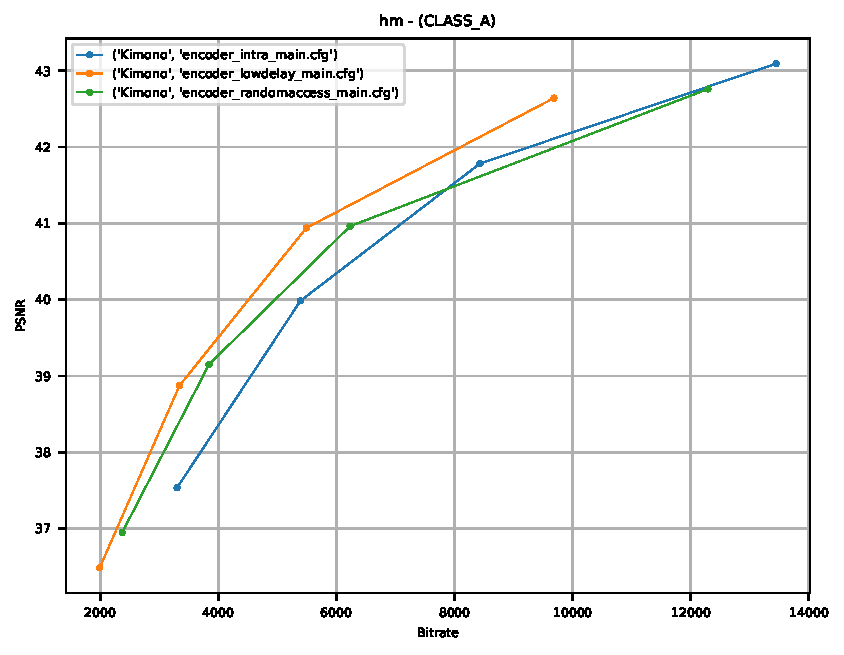
\includegraphics[scale=1.2]{%
/home/ridi/Desktop/Research_VVC_HM/results_2021_02_10_10_23_46/hm/encoder/hm_CLASS_A.pdf%
}}\end{figure}%
\newpage%
\begin{figure}[H] \centering{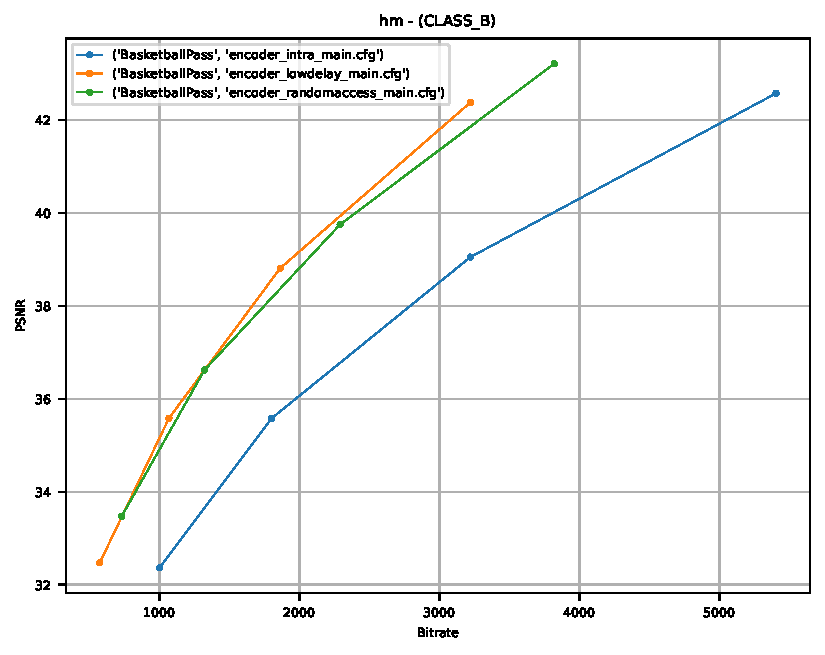
\includegraphics[scale=1.2]{%
/home/ridi/Desktop/Research_VVC_HM/results_2021_02_10_10_23_46/hm/encoder/hm_CLASS_B.pdf%
}}\end{figure}%
\newpage%
\begin{figure}[H] \centering{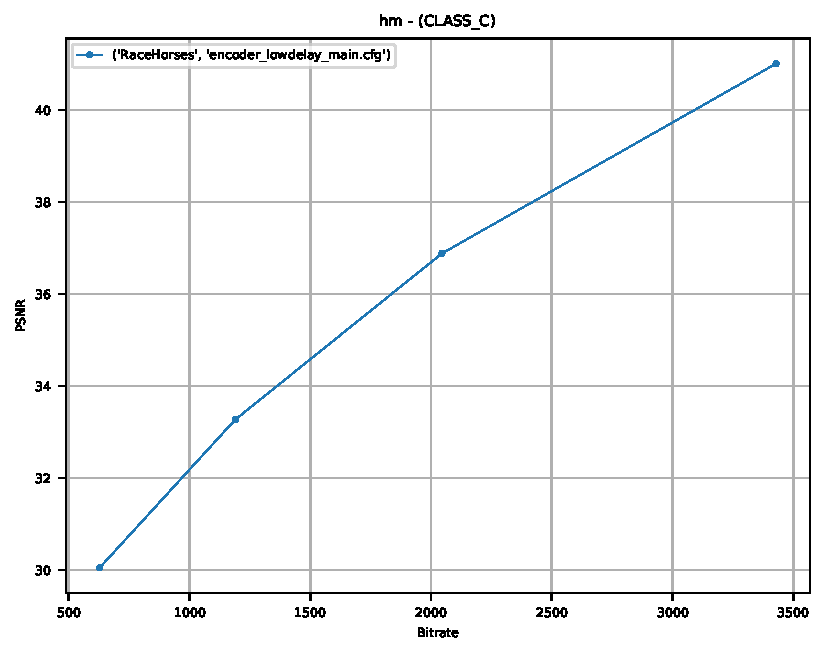
\includegraphics[scale=1.2]{%
/home/ridi/Desktop/Research_VVC_HM/results_2021_02_10_10_23_46/hm/encoder/hm_CLASS_C.pdf%
}}\end{figure}%
\newpage%
\subsubsection{Config Name: encoder\_intra\_main.cfg, Class Name: CLASS\_A}%
\label{ssubsec:ConfigNameencoderintramain.cfg,ClassNameCLASSA}%
\begin{longtabu}{| X[l] | X[l] |}%
\caption{%
Hotpots By Class (Kimono, QP =32)%
}%
\hline%
&\\%
\textbf{Class}&\textbf{CPU Time (\%)}\\%
&\\%
\hline%
\endhead%
xRateDistOptQuant&17.512\\%
\hline%
xPredIntraAng&9.764\\%
\hline%
xIntraCodingTUBlock&7.446\\%
\hline%
xCalcHADs4x4&2.243\\%
\hline%
&\\%
\hline%
estIntraPredLumaQT&2.13\\%
\hline%
initIntraPatternChType&1.923\\%
\hline%
estBit&1.904\\%
\hline%
codeCoeffNxN&1.489\\%
\hline%
&\\%
\hline%
codeIntraDirLumaAng&1.338\\%
\hline%
xRecurIntraCodingLumaQT&1.301\\%
\hline%
getIntraDirPredictor&1.301\\%
\hline%
predIntraAng&1.131\\%
\hline%
&\\%
\hline%
estLastSignificantPositionBit&1.093\\%
\hline%
xGetSSE8&0.961\\%
\hline%
xGetSSE16&0.924\\%
\hline%
encodeBin&0.905\\%
\hline%
&\\%
\hline%
xDeQuant&0.886\\%
\hline%
xT&0.867\\%
\hline%
xIT&0.811\\%
\hline%
getSigCtxInc&0.792\\%
\hline%
\end{longtabu}%
\newpage%
\begin{longtabu}{| X[l] | X[l] |}%
\caption{%
Hotspots By Function\newline%
 Config Name: encoder\_intra\_main.cfg,\newline%
 Class Name: CLASS\_A\newline%
 (Kimono, QP =32)%
}%
\hline%
&\\%
\textbf{Function}&\textbf{CPU Time}\\%
&\\%
\hline%
\endhead%
TComTrQuant::xRateDistOptQuant&3.716086\\%
\hline%
TComPrediction::xPredIntraAng&2.072018\\%
\hline%
TEncSearch::xIntraCodingTUBlock&1.580011\\%
\hline%
\_\_memmove\_avx\_unaligned\_erms&0.961984\\%
\hline%
&\\%
\hline%
TComRdCost::xCalcHADs4x4&0.476007\\%
\hline%
partialButterflyInverse32&0.451992\\%
\hline%
TEncSearch::estIntraPredLumaQT&0.451979\\%
\hline%
fillReferenceSamples&0.420040\\%
\hline%
&\\%
\hline%
partialButterfly32&0.407983\\%
\hline%
TComPrediction::initIntraPatternChType&0.407958\\%
\hline%
\_\_memset\_avx2\_unaligned\_erms&0.404016\\%
\hline%
TEncSbac::estBit&0.403970\\%
\hline%
&\\%
\hline%
simdHADs8x8&0.376008\\%
\hline%
partialButterfly16&0.340043\\%
\hline%
TEncSbac::codeCoeffNxN&0.316016\\%
\hline%
partialButterfly8&0.307951\\%
\hline%
&\\%
\hline%
TEncSbac::codeIntraDirLumaAng&0.283981\\%
\hline%
TEncSearch::xRecurIntraCodingLumaQT&0.276011\\%
\hline%
TComDataCU::getIntraDirPredictor&0.275970\\%
\hline%
TComPrediction::predIntraAng&0.239972\\%
\hline%
\end{longtabu}%
\newpage%
\begin{longtabu}{| X[l] | X[l] |}%
\caption{%
Memory Consumption\newline%
 Config Name: encoder\_intra\_main.cfg,\newline%
 Class Name: CLASS\_A\newline%
 (Kimono, QP =32)%
}%
\hline%
&\\%
\textbf{Function}&\textbf{Allocation/Deallocation Delta}\\%
&\\%
\hline%
\endhead%
func@0x8f3f0&72704.000000\\%
\hline%
main&4096.000000\\%
\hline%
\_\_libc\_csu\_init&1040.000000\\%
\hline%
\_\_static\_initialization\_and\_destruction\_0.constprop.69&1040.000000\\%
\hline%
&\\%
\hline%
EnvVar::EnvVar&690.000000\\%
\hline%
\_\_register\_frame&480.000000\\%
\hline%
\_GLOBAL\_\_sub\_I\_\_ZN3SEI19prefix\_sei\_messagesE&212.000000\\%
\hline%
indentNewLines&210.000000\\%
\hline%
&\\%
\hline%
TAppEncCfg::parseCfg&0.0\\%
\hline%
TAppEncCfg::xCheckParameter&0.0\\%
\hline%
TAppEncTop::encode&0.0\\%
\hline%
TAppEncTop::xGetBuffer&0.0\\%
\hline%
&\\%
\hline%
TComCUMvField::create&0.0\\%
\hline%
TComDataCU::create&0.0\\%
\hline%
TComLoopFilter::create&0.0\\%
\hline%
TComOutputBitstream::addSubstream&0.0\\%
\hline%
&\\%
\hline%
TComOutputBitstream::write&0.0\\%
\hline%
TComPic::create&0.0\\%
\hline%
TComPic::prepareForReconstruction&0.0\\%
\hline%
TComPicSym::TComPicSym&0.0\\%
\hline%
\end{longtabu}%
\newpage%
\begin{longtabu}{| X[l] | X[l] | X[l] | X[l] | X[l] | X[l] | X[l] |}%
\caption{%
Performance Snapshot\newline%
 Config Name: encoder\_intra\_main.cfg,\newline%
 Class Name: CLASS\_A\newline%
%
}%
\hline%
&&&&&&\\%
\textbf{Seq Name}&\textbf{IPC}&\textbf{Effective Logical Core Utilization}&\textbf{Effective Physical Core Utilization}&\textbf{Microarchitecture Usage}&\textbf{Vectorization}&\textbf{GPU Active Time}\\%
&&&&&&\\%
\hline%
\endhead%
Kimono\newline%
 QP = 22&2.108&14.6\% (1.165 out of 8)&28.0\% (1.120 out of 4)&56.7\% of Pipeline Slots&1.1\% of Packed FP Operations&0.9\%\\%
\hline%
Kimono\newline%
 QP = 37&2.230&14.9\% (1.193 out of 8)&28.6\% (1.143 out of 4)&59.1\% of Pipeline Slots&0.2\% of Packed FP Operations&3.1\%\\%
\hline%
Kimono\newline%
 QP = 32&2.275&14.4\% (1.151 out of 8)&27.8\% (1.111 out of 4)&61.1\% of Pipeline Slots&0.4\% of Packed FP Operations&0.9\%\\%
\hline%
Kimono\newline%
 QP = 27&2.137&15.5\% (1.243 out of 8)&29.5\% (1.181 out of 4)&58.4\% of Pipeline Slots&0.6\% of Packed FP Operations&0.9\%\\%
\hline%
\end{longtabu}%
\begin{longtabu}{| X[l] | X[l] | X[l] | X[l] | X[l] | X[l] | X[l] |}%
\caption{%
Instruction Mix\newline%
 Config Name: encoder\_intra\_main.cfg,\newline%
 Class Name: CLASS\_A\newline%
%
}%
\hline%
&&&&&&\\%
\textbf{Seq Name}&\textbf{SP FLOPs}&\textbf{DP FLOPs}&\textbf{x87 FLOPs}&\textbf{Non{-}FP}&\textbf{FP Arith/Mem Rd Instr. Ratio}&\textbf{FP Arith/Mem Wr Instr. Ratio}\\%
&&&&&&\\%
\hline%
\endhead%
Kimono\newline%
 QP = 22&0.0\% of uOps&1.1\% of uOps&0.1\% of uOps&98.8\% of uOps&0.045&0.093\\%
\hline%
Kimono\newline%
 QP = 37&0.0\% of uOps&1.0\% of uOps&0.1\% of uOps&98.9\% of uOps&0.041&0.083\\%
\hline%
Kimono\newline%
 QP = 32&0.0\% of uOps&1.0\% of uOps&0.1\% of uOps&98.9\% of uOps&0.041&0.083\\%
\hline%
Kimono\newline%
 QP = 27&0.0\% of uOps&1.0\% of uOps&0.1\% of uOps&98.9\% of uOps&0.041&0.083\\%
\hline%
\end{longtabu}%
\newpage%
\begin{longtabu}{| X[l] | X[l] | X[l] | X[l] | X[l] | X[l] |}%
\caption{%
GPU Usage\newline%
 Config Name: encoder\_intra\_main.cfg,\newline%
 Class Name: CLASS\_A\newline%
%
}%
\hline%
&&&&&\\%
\textbf{Seq Name}&\textbf{GPU Utilization when Busy}&\textbf{Active}&\textbf{Stalled}&\textbf{Idle}&\textbf{Occupancy}\\%
&&&&&\\%
\hline%
\endhead%
Kimono\newline%
 QP = 22&21.6\%&21.6\%&27.8\%&50.6\%&32.3\% of peak value\\%
\hline%
Kimono\newline%
 QP = 37&60.5\%&60.5\%&21.6\%&17.9\%&65.9\% of peak value\\%
\hline%
Kimono\newline%
 QP = 32&22.5\%&22.5\%&28.8\%&48.7\%&33.2\% of peak value\\%
\hline%
Kimono\newline%
 QP = 27&17.4\%&17.4\%&29.0\%&53.5\%&28.6\% of peak value\\%
\hline%
\end{longtabu}%
\begin{longtabu}{| X[l] | X[l] | X[l] | X[l] | X[l] | X[l] | X[l] | X[l] | X[l] |}%
\caption{%
Memory Access Analysis\newline%
 Config Name: encoder\_intra\_main.cfg,\newline%
 Class Name: CLASS\_A\newline%
%
}%
\hline%
&&&&&&&&\\%
\textbf{Seq Name}&\textbf{CPU Time}&\textbf{L1 Bound}&\textbf{L2 Bound}&\textbf{L3 Bound}&\textbf{DRAM Bound}&\textbf{Store Bound}&\textbf{LLC Miss Count}&\textbf{Average Latency (cycles)}\\%
&&&&&&&&\\%
\hline%
\endhead%
Kimono\newline%
 QP = 22&29.233s&5.0\% of Clockticks&0.4\% of Clockticks&0.5\% of Clockticks&0.2\% of Clockticks&0.8\% of Clockticks&0&9\\%
\hline%
Kimono\newline%
 QP = 37&20.539s&4.0\% of Clockticks&0.5\% of Clockticks&0.4\% of Clockticks&0.2\% of Clockticks&1.0\% of Clockticks&0&9\\%
\hline%
Kimono\newline%
 QP = 32&22.938s&4.2\% of Clockticks&0.5\% of Clockticks&0.5\% of Clockticks&0.0\% of Clockticks&1.1\% of Clockticks&0&9\\%
\hline%
Kimono\newline%
 QP = 27&24.784s&4.4\% of Clockticks&0.5\% of Clockticks&0.4\% of Clockticks&0.1\% of Clockticks&0.9\% of Clockticks&0&9\\%
\hline%
\end{longtabu}%
\newpage%
\begin{longtabu}{| X[l] | X[l] | X[l] | X[l] | X[l] | X[l] | X[l] |}%
\caption{%
Micro Architecture Exploration\newline%
 Config Name: encoder\_intra\_main.cfg,\newline%
 Class Name: CLASS\_A\newline%
%
}%
\hline%
&&&&&&\\%
\textbf{Seq Name}&\textbf{Clockticks}&\textbf{Instructions Retired}&\textbf{CPI Rate}&\textbf{Bad Speculation}&\textbf{Branch Mispredict}&\textbf{Vector Capacity Usage (FPU)}\\%
&&&&&&\\%
\hline%
\endhead%
Kimono\newline%
 QP = 22&66,952,800,000&160,651,800,000&0.417&9.6\% of Pipeline Slots&9.5\% of Pipeline Slots&24.7\%\\%
\hline%
Kimono\newline%
 QP = 37&49,671,000,000&127,409,400,000&0.390&5.3\% of Pipeline Slots&5.3\% of Pipeline Slots&24.5\%\\%
\hline%
Kimono\newline%
 QP = 32&53,238,600,000&132,447,600,000&0.402&5.8\% of Pipeline Slots&5.7\% of Pipeline Slots&24.5\%\\%
\hline%
Kimono\newline%
 QP = 27&57,843,000,000&140,349,600,000&0.412&7.0\% of Pipeline Slots&6.9\% of Pipeline Slots&24.6\%\\%
\hline%
\end{longtabu}%
\begin{longtabu}{| X[l] | X[l] | X[l] | X[l] | X[l] | X[l] | X[l] |}%
\caption{%
Front{-}End Bound Analysis\newline%
 Config Name: encoder\_intra\_main.cfg,\newline%
 Class Name: CLASS\_A\newline%
%
}%
\hline%
&&&&&&\\%
\textbf{Seq Name}&\textbf{Front{-}End Bound}&\textbf{Front{-}End Latency}&\textbf{ICache Misses}&\textbf{ITLB Overhead}&\textbf{Branch Resteers}&\textbf{Front{-}End Bandwidth}\\%
&&&&&&\\%
\hline%
\endhead%
Kimono\newline%
 QP = 22&19.7\% of Pipeline Slots&7.1\% of Pipeline Slots&2.7\% of Clockticks&0.2\% of Clockticks&4.2\% of Clockticks&12.6\% of Pipeline Slots\\%
\hline%
Kimono\newline%
 QP = 37&18.2\% of Pipeline Slots&5.7\% of Pipeline Slots&2.4\% of Clockticks&0.2\% of Clockticks&2.4\% of Clockticks&12.5\% of Pipeline Slots\\%
\hline%
Kimono\newline%
 QP = 32&19.2\% of Pipeline Slots&7.0\% of Pipeline Slots&2.8\% of Clockticks&1.0\% of Clockticks&3.6\% of Clockticks&12.3\% of Pipeline Slots\\%
\hline%
Kimono\newline%
 QP = 27&21.1\% of Pipeline Slots&8.1\% of Pipeline Slots&3.2\% of Clockticks&1.8\% of Clockticks&4.9\% of Clockticks&13.0\% of Pipeline Slots\\%
\hline%
\end{longtabu}%
\newpage%
\begin{longtabu}{| X[l] | X[l] | X[l] | X[l] | X[l] | X[l] | X[l] | X[l] |}%
\caption{%
Back{-}End Bound Analysis\newline%
 Config Name: encoder\_intra\_main.cfg,\newline%
 Class Name: CLASS\_A\newline%
%
}%
\hline%
&&&&&&&\\%
\textbf{Seq Name}&\textbf{Back{-}End Bound}&\textbf{L1 Bound}&\textbf{L2 Bound}&\textbf{L3 Bound}&\textbf{DRAM Bound}&\textbf{Store Bound}&\textbf{Store Latency}\\%
&&&&&&&\\%
\hline%
\endhead%
Kimono\newline%
 QP = 22&9.0\% of Pipeline Slots&5.1\% of Clockticks&0.4\% of Clockticks&0.4\% of Clockticks&0.0\% of Clockticks&0.6\% of Clockticks&8.7\% of Clockticks\\%
\hline%
Kimono\newline%
 QP = 37&10.1\% of Pipeline Slots&4.1\% of Clockticks&0.4\% of Clockticks&0.3\% of Clockticks&0.3\% of Clockticks&1.1\% of Clockticks&11.7\% of Clockticks\\%
\hline%
Kimono\newline%
 QP = 32&11.4\% of Pipeline Slots&4.4\% of Clockticks&0.4\% of Clockticks&0.6\% of Clockticks&0.2\% of Clockticks&0.9\% of Clockticks&11.2\% of Clockticks\\%
\hline%
Kimono\newline%
 QP = 27&8.9\% of Pipeline Slots&5.1\% of Clockticks&0.5\% of Clockticks&0.5\% of Clockticks&0.0\% of Clockticks&0.9\% of Clockticks&10.2\% of Clockticks\\%
\hline%
\end{longtabu}%
\newpage

%
\subsubsection{Config Name: encoder\_intra\_main.cfg, Class Name: CLASS\_B}%
\label{ssubsec:ConfigNameencoderintramain.cfg,ClassNameCLASSB}%
\begin{longtabu}{| X[l] | X[l] |}%
\caption{%
Hotpots By Class (BasketballPass, QP =27)%
}%
\hline%
&\\%
\textbf{Class}&\textbf{CPU Time (\%)}\\%
&\\%
\hline%
\endhead%
xRateDistOptQuant&23.999\\%
\hline%
xPredIntraAng&12.802\\%
\hline%
codeCoeffNxN&4.0\\%
\hline%
xIntraCodingTUBlock&3.999\\%
\hline%
&\\%
\hline%
xPredIntraPlanar&3.6\\%
\hline%
getSigCtxInc&3.4\\%
\hline%
initIntraPatternChType&2.4\\%
\hline%
codeLastSignificantXY&2.4\\%
\hline%
&\\%
\hline%
xWriteCoefRemainExGolomb&2.0\\%
\hline%
xTransformSkip&2.0\\%
\hline%
estIntraPredLumaQT&1.999\\%
\hline%
resetBits&1.999\\%
\hline%
&\\%
\hline%
xQuant&1.802\\%
\hline%
xGetIntraBitsQT&1.2\\%
\hline%
rdpcmNxN&1.2\\%
\hline%
predIntraAng&1.2\\%
\hline%
&\\%
\hline%
xRecurIntraCodingLumaQT&1.2\\%
\hline%
codeIntraDirLumaAng&1.2\\%
\hline%
encodeBinsEP&1.2\\%
\hline%
copyState&1.2\\%
\hline%
\end{longtabu}%
\newpage%
\begin{longtabu}{| X[l] | X[l] |}%
\caption{%
Hotspots By Function\newline%
 Config Name: encoder\_intra\_main.cfg,\newline%
 Class Name: CLASS\_B\newline%
 (BasketballPass, QP =27)%
}%
\hline%
&\\%
\textbf{Function}&\textbf{CPU Time}\\%
&\\%
\hline%
\endhead%
TComTrQuant::xRateDistOptQuant&0.239986\\%
\hline%
TComPrediction::xPredIntraAng&0.128018\\%
\hline%
\_\_memmove\_avx\_unaligned\_erms&0.067984\\%
\hline%
partialButterfly32&0.051953\\%
\hline%
&\\%
\hline%
TEncSbac::codeCoeffNxN&0.039997\\%
\hline%
TEncSearch::xIntraCodingTUBlock&0.039990\\%
\hline%
TComPrediction::xPredIntraPlanar&0.036003\\%
\hline%
TComTrQuant::getSigCtxInc&0.033997\\%
\hline%
&\\%
\hline%
TComPrediction::initIntraPatternChType&0.024002\\%
\hline%
TEncSbac::codeLastSignificantXY&0.023996\\%
\hline%
TEncSbac::xWriteCoefRemainExGolomb&0.020002\\%
\hline%
TComTrQuant::xTransformSkip&0.020001\\%
\hline%
&\\%
\hline%
partialButterfly4&0.020000\\%
\hline%
TEncSearch::estIntraPredLumaQT&0.019994\\%
\hline%
TComTrQuant::xQuant&0.018020\\%
\hline%
TEncSearch::xGetIntraBitsQT&0.012004\\%
\hline%
&\\%
\hline%
TComTrQuant::rdpcmNxN&0.012003\\%
\hline%
TComBitCounter::resetBits&0.012002\\%
\hline%
TComPrediction::predIntraAng&0.012002\\%
\hline%
partialButterflyInverse8&0.012002\\%
\hline%
\end{longtabu}%
\newpage%
\begin{longtabu}{| X[l] | X[l] |}%
\caption{%
Memory Consumption\newline%
 Config Name: encoder\_intra\_main.cfg,\newline%
 Class Name: CLASS\_B\newline%
 (BasketballPass, QP =27)%
}%
\hline%
&\\%
\textbf{Function}&\textbf{Allocation/Deallocation Delta}\\%
&\\%
\hline%
\endhead%
func@0x8f3f0&72704.000000\\%
\hline%
main&4096.000000\\%
\hline%
\_\_libc\_csu\_init&1040.000000\\%
\hline%
\_\_static\_initialization\_and\_destruction\_0.constprop.69&1040.000000\\%
\hline%
&\\%
\hline%
EnvVar::EnvVar&690.000000\\%
\hline%
\_\_register\_frame&480.000000\\%
\hline%
\_GLOBAL\_\_sub\_I\_\_ZN3SEI19prefix\_sei\_messagesE&212.000000\\%
\hline%
indentNewLines&210.000000\\%
\hline%
&\\%
\hline%
TAppEncCfg::parseCfg&0.0\\%
\hline%
TAppEncCfg::xCheckParameter&0.0\\%
\hline%
TAppEncTop::encode&0.0\\%
\hline%
TAppEncTop::xGetBuffer&0.0\\%
\hline%
&\\%
\hline%
TComCUMvField::create&0.0\\%
\hline%
TComDataCU::create&0.0\\%
\hline%
TComLoopFilter::create&0.0\\%
\hline%
TComOutputBitstream::addSubstream&0.0\\%
\hline%
&\\%
\hline%
TComOutputBitstream::write&0.0\\%
\hline%
TComPic::create&0.0\\%
\hline%
TComPic::prepareForReconstruction&0.0\\%
\hline%
TComPicSym::TComPicSym&0.0\\%
\hline%
\end{longtabu}%
\newpage%
\begin{longtabu}{| X[l] | X[l] | X[l] | X[l] | X[l] | X[l] | X[l] |}%
\caption{%
Performance Snapshot\newline%
 Config Name: encoder\_intra\_main.cfg,\newline%
 Class Name: CLASS\_B\newline%
%
}%
\hline%
&&&&&&\\%
\textbf{Seq Name}&\textbf{IPC}&\textbf{Effective Logical Core Utilization}&\textbf{Effective Physical Core Utilization}&\textbf{Microarchitecture Usage}&\textbf{Vectorization}&\textbf{GPU Active Time}\\%
&&&&&&\\%
\hline%
\endhead%
BasketballPass\newline%
 QP = 37&2.078&16.2\% (1.294 out of 8)&31.3\% (1.252 out of 4)&54.8\% of Pipeline Slots&0.7\% of Packed FP Operations&2.0\%\\%
\hline%
BasketballPass\newline%
 QP = 32&2.065&15.4\% (1.232 out of 8)&30.0\% (1.199 out of 4)&55.4\% of Pipeline Slots&1.1\% of Packed FP Operations&1.4\%\\%
\hline%
BasketballPass\newline%
 QP = 22&1.978&15.0\% (1.202 out of 8)&28.0\% (1.118 out of 4)&53.4\% of Pipeline Slots&2.6\% of Packed FP Operations&1.3\%\\%
\hline%
BasketballPass\newline%
 QP = 27&2.252&14.1\% (1.126 out of 8)&27.4\% (1.097 out of 4)&55.5\% of Pipeline Slots&1.7\% of Packed FP Operations&1.2\%\\%
\hline%
\end{longtabu}%
\begin{longtabu}{| X[l] | X[l] | X[l] | X[l] | X[l] | X[l] | X[l] |}%
\caption{%
Instruction Mix\newline%
 Config Name: encoder\_intra\_main.cfg,\newline%
 Class Name: CLASS\_B\newline%
%
}%
\hline%
&&&&&&\\%
\textbf{Seq Name}&\textbf{SP FLOPs}&\textbf{DP FLOPs}&\textbf{x87 FLOPs}&\textbf{Non{-}FP}&\textbf{FP Arith/Mem Rd Instr. Ratio}&\textbf{FP Arith/Mem Wr Instr. Ratio}\\%
&&&&&&\\%
\hline%
\endhead%
BasketballPass\newline%
 QP = 37&0.0\% of uOps&1.1\% of uOps&0.1\% of uOps&98.9\% of uOps&0.045&0.090\\%
\hline%
BasketballPass\newline%
 QP = 32&0.0\% of uOps&1.0\% of uOps&0.1\% of uOps&98.9\% of uOps&0.042&0.085\\%
\hline%
BasketballPass\newline%
 QP = 22&0.0\% of uOps&1.2\% of uOps&0.1\% of uOps&98.7\% of uOps&0.051&0.105\\%
\hline%
BasketballPass\newline%
 QP = 27&0.0\% of uOps&1.2\% of uOps&0.1\% of uOps&98.8\% of uOps&0.046&0.097\\%
\hline%
\end{longtabu}%
\newpage%
\begin{longtabu}{| X[l] | X[l] | X[l] | X[l] | X[l] | X[l] |}%
\caption{%
GPU Usage\newline%
 Config Name: encoder\_intra\_main.cfg,\newline%
 Class Name: CLASS\_B\newline%
%
}%
\hline%
&&&&&\\%
\textbf{Seq Name}&\textbf{GPU Utilization when Busy}&\textbf{Active}&\textbf{Stalled}&\textbf{Idle}&\textbf{Occupancy}\\%
&&&&&\\%
\hline%
\endhead%
BasketballPass\newline%
 QP = 37&17.9\%&17.9\%&32.2\%&49.9\%&30.1\% of peak value\\%
\hline%
BasketballPass\newline%
 QP = 32&18.1\%&18.1\%&30.0\%&52.0\%&30.5\% of peak value\\%
\hline%
BasketballPass\newline%
 QP = 22&14.2\%&14.2\%&29.0\%&56.8\%&25.5\% of peak value\\%
\hline%
BasketballPass\newline%
 QP = 27&16.8\%&16.8\%&29.8\%&53.4\%&28.1\% of peak value\\%
\hline%
\end{longtabu}%
\begin{longtabu}{| X[l] | X[l] | X[l] | X[l] | X[l] | X[l] | X[l] | X[l] | X[l] |}%
\caption{%
Memory Access Analysis\newline%
 Config Name: encoder\_intra\_main.cfg,\newline%
 Class Name: CLASS\_B\newline%
%
}%
\hline%
&&&&&&&&\\%
\textbf{Seq Name}&\textbf{CPU Time}&\textbf{L1 Bound}&\textbf{L2 Bound}&\textbf{L3 Bound}&\textbf{DRAM Bound}&\textbf{Store Bound}&\textbf{LLC Miss Count}&\textbf{Average Latency (cycles)}\\%
&&&&&&&&\\%
\hline%
\endhead%
BasketballPass\newline%
 QP = 37&0.773s&4.4\% of Clockticks&0.9\% of Clockticks&0.0\% of Clockticks&0.0\% of Clockticks&0.9\% of Clockticks&0&9\\%
\hline%
BasketballPass\newline%
 QP = 32&0.898s&5.3\% of Clockticks&0.0\% of Clockticks&0.8\% of Clockticks&0.0\% of Clockticks&0.0\% of Clockticks&0&10\\%
\hline%
BasketballPass\newline%
 QP = 22&1.219s&6.1\% of Clockticks&0.6\% of Clockticks&0.0\% of Clockticks&0.0\% of Clockticks&0.6\% of Clockticks&0&9\\%
\hline%
BasketballPass\newline%
 QP = 27&1.499s&4.5\% of Clockticks&0.0\% of Clockticks&0.6\% of Clockticks&0.0\% of Clockticks&0.6\% of Clockticks&0&9\\%
\hline%
\end{longtabu}%
\newpage%
\begin{longtabu}{| X[l] | X[l] | X[l] | X[l] | X[l] | X[l] | X[l] |}%
\caption{%
Micro Architecture Exploration\newline%
 Config Name: encoder\_intra\_main.cfg,\newline%
 Class Name: CLASS\_B\newline%
%
}%
\hline%
&&&&&&\\%
\textbf{Seq Name}&\textbf{Clockticks}&\textbf{Instructions Retired}&\textbf{CPI Rate}&\textbf{Bad Speculation}&\textbf{Branch Mispredict}&\textbf{Vector Capacity Usage (FPU)}\\%
&&&&&&\\%
\hline%
\endhead%
BasketballPass\newline%
 QP = 37&2,746,800,000&6,699,600,000&0.410&7.4\% of Pipeline Slots&7.4\% of Pipeline Slots&25.0\%\\%
\hline%
BasketballPass\newline%
 QP = 32&3,142,800,000&7,410,600,000&0.424&8.2\% of Pipeline Slots&8.2\% of Pipeline Slots&25.0\%\\%
\hline%
BasketballPass\newline%
 QP = 22&4,329,000,000&9,484,200,000&0.456&14.8\% of Pipeline Slots&14.8\% of Pipeline Slots&25.0\%\\%
\hline%
BasketballPass\newline%
 QP = 27&3,650,400,000&8,310,600,000&0.439&11.5\% of Pipeline Slots&11.5\% of Pipeline Slots&25.0\%\\%
\hline%
\end{longtabu}%
\begin{longtabu}{| X[l] | X[l] | X[l] | X[l] | X[l] | X[l] | X[l] |}%
\caption{%
Front{-}End Bound Analysis\newline%
 Config Name: encoder\_intra\_main.cfg,\newline%
 Class Name: CLASS\_B\newline%
%
}%
\hline%
&&&&&&\\%
\textbf{Seq Name}&\textbf{Front{-}End Bound}&\textbf{Front{-}End Latency}&\textbf{ICache Misses}&\textbf{ITLB Overhead}&\textbf{Branch Resteers}&\textbf{Front{-}End Bandwidth}\\%
&&&&&&\\%
\hline%
\endhead%
BasketballPass\newline%
 QP = 37&18.7\% of Pipeline Slots&5.9\% of Pipeline Slots&2.0\% of Clockticks&0.4\% of Clockticks&2.0\% of Clockticks&12.8\% of Pipeline Slots\\%
\hline%
BasketballPass\newline%
 QP = 32&18.0\% of Pipeline Slots&5.2\% of Pipeline Slots&1.7\% of Clockticks&0.2\% of Clockticks&1.7\% of Clockticks&12.9\% of Pipeline Slots\\%
\hline%
BasketballPass\newline%
 QP = 22&21.6\% of Pipeline Slots&7.7\% of Pipeline Slots&1.2\% of Clockticks&0.2\% of Clockticks&4.3\% of Clockticks&13.8\% of Pipeline Slots\\%
\hline%
BasketballPass\newline%
 QP = 27&18.5\% of Pipeline Slots&7.4\% of Pipeline Slots&1.5\% of Clockticks&0.1\% of Clockticks&3.6\% of Clockticks&11.1\% of Pipeline Slots\\%
\hline%
\end{longtabu}%
\newpage%
\begin{longtabu}{| X[l] | X[l] | X[l] | X[l] | X[l] | X[l] | X[l] | X[l] |}%
\caption{%
Back{-}End Bound Analysis\newline%
 Config Name: encoder\_intra\_main.cfg,\newline%
 Class Name: CLASS\_B\newline%
%
}%
\hline%
&&&&&&&\\%
\textbf{Seq Name}&\textbf{Back{-}End Bound}&\textbf{L1 Bound}&\textbf{L2 Bound}&\textbf{L3 Bound}&\textbf{DRAM Bound}&\textbf{Store Bound}&\textbf{Store Latency}\\%
&&&&&&&\\%
\hline%
\endhead%
BasketballPass\newline%
 QP = 37&12.5\% of Pipeline Slots&3.9\% of Clockticks&0.0\% of Clockticks&0.0\% of Clockticks&0.0\% of Clockticks&0.0\% of Clockticks&7.1\% of Clockticks\\%
\hline%
BasketballPass\newline%
 QP = 32&14.5\% of Pipeline Slots&5.2\% of Clockticks&0.0\% of Clockticks&0.0\% of Clockticks&0.0\% of Clockticks&0.0\% of Clockticks&7.9\% of Clockticks\\%
\hline%
BasketballPass\newline%
 QP = 22&4.4\% of Pipeline Slots&6.2\% of Clockticks&0.0\% of Clockticks&0.0\% of Clockticks&0.0\% of Clockticks&0.0\% of Clockticks&5.7\% of Clockticks\\%
\hline%
BasketballPass\newline%
 QP = 27&16.1\% of Pipeline Slots&5.9\% of Clockticks&0.0\% of Clockticks&0.0\% of Clockticks&0.0\% of Clockticks&0.0\% of Clockticks&6.8\% of Clockticks\\%
\hline%
\end{longtabu}%
\newpage

%
\subsubsection{Config Name: encoder\_intra\_main.cfg, Class Name: CLASS\_C}%
\label{ssubsec:ConfigNameencoderintramain.cfg,ClassNameCLASSC}%
\begin{longtabu}{| X[l] | X[l] |}%
\caption{%
Hotpots By Class (RaceHorses, QP =22)%
}%
\hline%
&\\%
\textbf{Class}&\textbf{CPU Time (\%)}\\%
&\\%
\hline%
\endhead%
xRateDistOptQuant&30.051\\%
\hline%
codeCoeffNxN&12.994\\%
\hline%
xPredIntraAng&5.482\\%
\hline%
xIntraCodingTUBlock&3.857\\%
\hline%
&\\%
\hline%
getSigCtxInc&3.655\\%
\hline%
xWriteCoefRemainExGolomb&2.335\\%
\hline%
xGetSSE32&2.233\\%
\hline%
xCalcHADs4x4&2.031\\%
\hline%
&\\%
\hline%
encodeBin&2.03\\%
\hline%
initIntraPatternChType&1.422\\%
\hline%
getPUAboveRight&1.218\\%
\hline%
xEncSubdivCbfQT&1.218\\%
\hline%
&\\%
\hline%
getAddr&1.218\\%
\hline%
xT&1.015\\%
\hline%
xITransformSkip&1.015\\%
\hline%
encodeBinsEP&1.015\\%
\hline%
&\\%
\hline%
estBit&0.812\\%
\hline%
copyState&0.812\\%
\hline%
xGetSSE8&0.812\\%
\hline%
getPUBelowLeft&0.61\\%
\hline%
\end{longtabu}%
\newpage%
\begin{longtabu}{| X[l] | X[l] |}%
\caption{%
Hotspots By Function\newline%
 Config Name: encoder\_intra\_main.cfg,\newline%
 Class Name: CLASS\_C\newline%
 (RaceHorses, QP =22)%
}%
\hline%
&\\%
\textbf{Function}&\textbf{CPU Time}\\%
&\\%
\hline%
\endhead%
TComTrQuant::xRateDistOptQuant&0.592000\\%
\hline%
TEncSbac::codeCoeffNxN&0.255991\\%
\hline%
TComPrediction::xPredIntraAng&0.107987\\%
\hline%
TEncSearch::xIntraCodingTUBlock&0.075991\\%
\hline%
&\\%
\hline%
TComTrQuant::getSigCtxInc&0.072007\\%
\hline%
TEncSbac::xWriteCoefRemainExGolomb&0.045997\\%
\hline%
\_\_memset\_avx2\_unaligned\_erms&0.043999\\%
\hline%
TComRdCost::xGetSSE32&0.043995\\%
\hline%
&\\%
\hline%
\_\_memmove\_avx\_unaligned\_erms&0.040005\\%
\hline%
simdHADs8x8&0.040003\\%
\hline%
TComRdCost::xCalcHADs4x4&0.040001\\%
\hline%
TEncBinCABACCounter::encodeBin&0.039989\\%
\hline%
&\\%
\hline%
partialButterflyInverse4&0.031998\\%
\hline%
TComPrediction::initIntraPatternChType&0.028007\\%
\hline%
TComDataCU::getPUAboveRight&0.024004\\%
\hline%
TEncSearch::xEncSubdivCbfQT&0.024002\\%
\hline%
&\\%
\hline%
TComYuv::getAddr&0.023997\\%
\hline%
partialButterfly16&0.023994\\%
\hline%
partialButterflyInverse8&0.020003\\%
\hline%
TComTrQuant::xT&0.020002\\%
\hline%
\end{longtabu}%
\newpage%
\begin{longtabu}{| X[l] | X[l] |}%
\caption{%
Memory Consumption\newline%
 Config Name: encoder\_intra\_main.cfg,\newline%
 Class Name: CLASS\_C\newline%
 (RaceHorses, QP =22)%
}%
\hline%
&\\%
\textbf{Function}&\textbf{Allocation/Deallocation Delta}\\%
&\\%
\hline%
\endhead%
func@0x8f3f0&72704.000000\\%
\hline%
main&4096.000000\\%
\hline%
\_\_libc\_csu\_init&1040.000000\\%
\hline%
\_\_static\_initialization\_and\_destruction\_0.constprop.69&1040.000000\\%
\hline%
&\\%
\hline%
EnvVar::EnvVar&690.000000\\%
\hline%
\_\_register\_frame&480.000000\\%
\hline%
\_GLOBAL\_\_sub\_I\_\_ZN3SEI19prefix\_sei\_messagesE&212.000000\\%
\hline%
indentNewLines&210.000000\\%
\hline%
&\\%
\hline%
TAppEncCfg::parseCfg&0.0\\%
\hline%
TAppEncCfg::xCheckParameter&0.0\\%
\hline%
TAppEncTop::encode&0.0\\%
\hline%
TAppEncTop::xGetBuffer&0.0\\%
\hline%
&\\%
\hline%
TComCUMvField::create&0.0\\%
\hline%
TComDataCU::create&0.0\\%
\hline%
TComLoopFilter::create&0.0\\%
\hline%
TComOutputBitstream::addSubstream&0.0\\%
\hline%
&\\%
\hline%
TComOutputBitstream::write&0.0\\%
\hline%
TComPic::create&0.0\\%
\hline%
TComPic::prepareForReconstruction&0.0\\%
\hline%
TComPicSym::TComPicSym&0.0\\%
\hline%
\end{longtabu}%
\newpage%
\begin{longtabu}{| X[l] | X[l] | X[l] | X[l] | X[l] | X[l] | X[l] |}%
\caption{%
Performance Snapshot\newline%
 Config Name: encoder\_intra\_main.cfg,\newline%
 Class Name: CLASS\_C\newline%
%
}%
\hline%
&&&&&&\\%
\textbf{Seq Name}&\textbf{IPC}&\textbf{Effective Logical Core Utilization}&\textbf{Effective Physical Core Utilization}&\textbf{Microarchitecture Usage}&\textbf{Vectorization}&\textbf{GPU Active Time}\\%
&&&&&&\\%
\hline%
\endhead%
RaceHorses\newline%
 QP = 32&2.073&14.6\% (1.169 out of 8)&28.2\% (1.127 out of 4)&54.8\% of Pipeline Slots&1.6\% of Packed FP Operations&1.7\%\\%
\hline%
RaceHorses\newline%
 QP = 27&1.960&14.9\% (1.195 out of 8)&28.9\% (1.157 out of 4)&54.4\% of Pipeline Slots&2.4\% of Packed FP Operations&1.2\%\\%
\hline%
RaceHorses\newline%
 QP = 37&1.976&18.9\% (1.513 out of 8)&35.0\% (1.399 out of 4)&49.2\% of Pipeline Slots&1.0\% of Packed FP Operations&1.4\%\\%
\hline%
RaceHorses\newline%
 QP = 22&1.950&14.7\% (1.179 out of 8)&28.5\% (1.141 out of 4)&51.7\% of Pipeline Slots&2.8\% of Packed FP Operations&1.3\%\\%
\hline%
\end{longtabu}%
\begin{longtabu}{| X[l] | X[l] | X[l] | X[l] | X[l] | X[l] | X[l] |}%
\caption{%
Instruction Mix\newline%
 Config Name: encoder\_intra\_main.cfg,\newline%
 Class Name: CLASS\_C\newline%
%
}%
\hline%
&&&&&&\\%
\textbf{Seq Name}&\textbf{SP FLOPs}&\textbf{DP FLOPs}&\textbf{x87 FLOPs}&\textbf{Non{-}FP}&\textbf{FP Arith/Mem Rd Instr. Ratio}&\textbf{FP Arith/Mem Wr Instr. Ratio}\\%
&&&&&&\\%
\hline%
\endhead%
RaceHorses\newline%
 QP = 32&0.0\% of uOps&1.1\% of uOps&0.1\% of uOps&98.8\% of uOps&0.044&0.092\\%
\hline%
RaceHorses\newline%
 QP = 27&0.0\% of uOps&1.1\% of uOps&0.1\% of uOps&98.8\% of uOps&0.046&0.097\\%
\hline%
RaceHorses\newline%
 QP = 37&0.0\% of uOps&1.1\% of uOps&0.1\% of uOps&98.9\% of uOps&0.039&0.078\\%
\hline%
RaceHorses\newline%
 QP = 22&0.0\% of uOps&1.2\% of uOps&0.1\% of uOps&98.7\% of uOps&0.049&0.104\\%
\hline%
\end{longtabu}%
\newpage%
\begin{longtabu}{| X[l] | X[l] | X[l] | X[l] | X[l] | X[l] |}%
\caption{%
GPU Usage\newline%
 Config Name: encoder\_intra\_main.cfg,\newline%
 Class Name: CLASS\_C\newline%
%
}%
\hline%
&&&&&\\%
\textbf{Seq Name}&\textbf{GPU Utilization when Busy}&\textbf{Active}&\textbf{Stalled}&\textbf{Idle}&\textbf{Occupancy}\\%
&&&&&\\%
\hline%
\endhead%
RaceHorses\newline%
 QP = 32&16.4\%&16.4\%&30.1\%&53.5\%&28.2\% of peak value\\%
\hline%
RaceHorses\newline%
 QP = 27&16.6\%&16.6\%&32.1\%&51.3\%&29.2\% of peak value\\%
\hline%
RaceHorses\newline%
 QP = 37&15.4\%&15.4\%&31.0\%&53.6\%&27.4\% of peak value\\%
\hline%
RaceHorses\newline%
 QP = 22&21.5\%&21.5\%&29.6\%&48.9\%&33.6\% of peak value\\%
\hline%
\end{longtabu}%
\begin{longtabu}{| X[l] | X[l] | X[l] | X[l] | X[l] | X[l] | X[l] | X[l] | X[l] |}%
\caption{%
Memory Access Analysis\newline%
 Config Name: encoder\_intra\_main.cfg,\newline%
 Class Name: CLASS\_C\newline%
%
}%
\hline%
&&&&&&&&\\%
\textbf{Seq Name}&\textbf{CPU Time}&\textbf{L1 Bound}&\textbf{L2 Bound}&\textbf{L3 Bound}&\textbf{DRAM Bound}&\textbf{Store Bound}&\textbf{LLC Miss Count}&\textbf{Average Latency (cycles)}\\%
&&&&&&&&\\%
\hline%
\endhead%
RaceHorses\newline%
 QP = 32&1.117s&5.2\% of Clockticks&0.7\% of Clockticks&0.0\% of Clockticks&0.0\% of Clockticks&0.7\% of Clockticks&0&9\\%
\hline%
RaceHorses\newline%
 QP = 27&1.315s&6.0\% of Clockticks&0.5\% of Clockticks&0.0\% of Clockticks&0.0\% of Clockticks&0.5\% of Clockticks&0&9\\%
\hline%
RaceHorses\newline%
 QP = 37&0.887s&4.6\% of Clockticks&0.8\% of Clockticks&0.0\% of Clockticks&0.0\% of Clockticks&0.8\% of Clockticks&0&8\\%
\hline%
RaceHorses\newline%
 QP = 22&1.417s&6.7\% of Clockticks&0.0\% of Clockticks&0.5\% of Clockticks&0.0\% of Clockticks&0.5\% of Clockticks&0&8\\%
\hline%
\end{longtabu}%
\newpage%
\begin{longtabu}{| X[l] | X[l] | X[l] | X[l] | X[l] | X[l] | X[l] |}%
\caption{%
Micro Architecture Exploration\newline%
 Config Name: encoder\_intra\_main.cfg,\newline%
 Class Name: CLASS\_C\newline%
%
}%
\hline%
&&&&&&\\%
\textbf{Seq Name}&\textbf{Clockticks}&\textbf{Instructions Retired}&\textbf{CPI Rate}&\textbf{Bad Speculation}&\textbf{Branch Mispredict}&\textbf{Vector Capacity Usage (FPU)}\\%
&&&&&&\\%
\hline%
\endhead%
RaceHorses\newline%
 QP = 32&3,749,400,000&8,337,600,000&0.450&11.2\% of Pipeline Slots&11.2\% of Pipeline Slots&25.0\%\\%
\hline%
RaceHorses\newline%
 QP = 27&4,363,200,000&9,471,600,000&0.461&15.8\% of Pipeline Slots&15.8\% of Pipeline Slots&25.0\%\\%
\hline%
RaceHorses\newline%
 QP = 37&3,101,400,000&7,363,800,000&0.421&7.8\% of Pipeline Slots&7.8\% of Pipeline Slots&25.0\%\\%
\hline%
RaceHorses\newline%
 QP = 22&5,072,400,000&10,722,600,000&0.473&15.4\% of Pipeline Slots&15.4\% of Pipeline Slots&25.0\%\\%
\hline%
\end{longtabu}%
\begin{longtabu}{| X[l] | X[l] | X[l] | X[l] | X[l] | X[l] | X[l] |}%
\caption{%
Front{-}End Bound Analysis\newline%
 Config Name: encoder\_intra\_main.cfg,\newline%
 Class Name: CLASS\_C\newline%
%
}%
\hline%
&&&&&&\\%
\textbf{Seq Name}&\textbf{Front{-}End Bound}&\textbf{Front{-}End Latency}&\textbf{ICache Misses}&\textbf{ITLB Overhead}&\textbf{Branch Resteers}&\textbf{Front{-}End Bandwidth}\\%
&&&&&&\\%
\hline%
\endhead%
RaceHorses\newline%
 QP = 32&20.6\% of Pipeline Slots&7.5\% of Pipeline Slots&1.4\% of Clockticks&0.4\% of Clockticks&5.0\% of Clockticks&13.1\% of Pipeline Slots\\%
\hline%
RaceHorses\newline%
 QP = 27&21.2\% of Pipeline Slots&9.0\% of Pipeline Slots&1.2\% of Clockticks&0.2\% of Clockticks&6.1\% of Clockticks&12.2\% of Pipeline Slots\\%
\hline%
RaceHorses\newline%
 QP = 37&19.6\% of Pipeline Slots&7.0\% of Pipeline Slots&1.7\% of Clockticks&0.2\% of Clockticks&4.3\% of Clockticks&12.6\% of Pipeline Slots\\%
\hline%
RaceHorses\newline%
 QP = 22&20.5\% of Pipeline Slots&8.5\% of Pipeline Slots&2.1\% of Clockticks&0.2\% of Clockticks&5.8\% of Clockticks&12.0\% of Pipeline Slots\\%
\hline%
\end{longtabu}%
\newpage%
\begin{longtabu}{| X[l] | X[l] | X[l] | X[l] | X[l] | X[l] | X[l] | X[l] |}%
\caption{%
Back{-}End Bound Analysis\newline%
 Config Name: encoder\_intra\_main.cfg,\newline%
 Class Name: CLASS\_C\newline%
%
}%
\hline%
&&&&&&&\\%
\textbf{Seq Name}&\textbf{Back{-}End Bound}&\textbf{L1 Bound}&\textbf{L2 Bound}&\textbf{L3 Bound}&\textbf{DRAM Bound}&\textbf{Store Bound}&\textbf{Store Latency}\\%
&&&&&&&\\%
\hline%
\endhead%
RaceHorses\newline%
 QP = 32&9.0\% of Pipeline Slots&5.8\% of Clockticks&0.0\% of Clockticks&0.0\% of Clockticks&0.0\% of Clockticks&0.0\% of Clockticks&7.9\% of Clockticks\\%
\hline%
RaceHorses\newline%
 QP = 27&6.7\% of Pipeline Slots&6.2\% of Clockticks&0.0\% of Clockticks&0.0\% of Clockticks&0.0\% of Clockticks&0.0\% of Clockticks&5.7\% of Clockticks\\%
\hline%
RaceHorses\newline%
 QP = 37&12.1\% of Pipeline Slots&7.0\% of Clockticks&0.0\% of Clockticks&0.0\% of Clockticks&0.0\% of Clockticks&0.0\% of Clockticks&6.4\% of Clockticks\\%
\hline%
RaceHorses\newline%
 QP = 22&9.8\% of Pipeline Slots&6.4\% of Clockticks&0.0\% of Clockticks&0.0\% of Clockticks&0.0\% of Clockticks&0.0\% of Clockticks&4.9\% of Clockticks\\%
\hline%
\end{longtabu}%
\newpage

%
\subsubsection{Config Name: encoder\_lowdelay\_main.cfg, Class Name: CLASS\_A}%
\label{ssubsec:ConfigNameencoderlowdelaymain.cfg,ClassNameCLASSA}%
\begin{longtabu}{| X[l] | X[l] |}%
\caption{%
Hotpots By Class (Kimono, QP =32)%
}%
\hline%
&\\%
\textbf{Class}&\textbf{CPU Time (\%)}\\%
&\\%
\hline%
\endhead%
xRateDistOptQuant&17.932\\%
\hline%
xPredIntraAng&3.764\\%
\hline%
filter<(int)8, (bool)1, (bool)0, (bool)1>&3.313\\%
\hline%
xIntraCodingTUBlock&3.101\\%
\hline%
&\\%
\hline%
xEstimateInterResidualQT&2.843\\%
\hline%
filter<(int)8, (bool)0, (bool)1, (bool)0>&2.73\\%
\hline%
xCalcHADs4x4&2.332\\%
\hline%
xGetSSE16&1.683\\%
\hline%
&\\%
\hline%
estBit&1.564\\%
\hline%
filterCopy&1.405\\%
\hline%
xGetSSE8&1.272\\%
\hline%
codeCoeffNxN&1.153\\%
\hline%
&\\%
\hline%
xGetSSE32&1.113\\%
\hline%
initIntraPatternChType&0.861\\%
\hline%
xGetHADs&0.808\\%
\hline%
xGetExpGolombNumberOfBits&0.795\\%
\hline%
&\\%
\hline%
estLastSignificantPositionBit&0.795\\%
\hline%
filter<(int)4, (bool)0, (bool)1, (bool)0>&0.742\\%
\hline%
encodeBin&0.729\\%
\hline%
xT&0.716\\%
\hline%
\end{longtabu}%
\newpage%
\begin{longtabu}{| X[l] | X[l] |}%
\caption{%
Hotspots By Function\newline%
 Config Name: encoder\_lowdelay\_main.cfg,\newline%
 Class Name: CLASS\_A\newline%
 (Kimono, QP =32)%
}%
\hline%
&\\%
\textbf{Function}&\textbf{CPU Time}\\%
&\\%
\hline%
\endhead%
TComTrQuant::xRateDistOptQuant&5.411486\\%
\hline%
\_\_memmove\_avx\_unaligned\_erms&1.157995\\%
\hline%
TComPrediction::xPredIntraAng&1.135853\\%
\hline%
TComInterpolationFilter::filter<(int)8, (bool)1, (bool)0, (bool)1>&0.999926\\%
\hline%
&\\%
\hline%
simdHADs8x8&0.983849\\%
\hline%
TEncSearch::xIntraCodingTUBlock&0.935862\\%
\hline%
\_\_memset\_avx2\_unaligned\_erms&0.859978\\%
\hline%
TEncSearch::xEstimateInterResidualQT&0.857948\\%
\hline%
&\\%
\hline%
TComInterpolationFilter::filter<(int)8, (bool)0, (bool)1, (bool)0>&0.823910\\%
\hline%
TComRdCost::xCalcHADs4x4&0.703899\\%
\hline%
partialButterfly32&0.599969\\%
\hline%
\_Z15simd8x8HAD1D32bPDv2\_xS0\_&0.543914\\%
\hline%
&\\%
\hline%
TComRdCost::xGetSSE16&0.507970\\%
\hline%
partialButterflyInverse32&0.483965\\%
\hline%
TEncSbac::estBit&0.471968\\%
\hline%
partialButterfly8&0.439945\\%
\hline%
&\\%
\hline%
TComInterpolationFilter::filterCopy&0.423913\\%
\hline%
partialButterfly16&0.411991\\%
\hline%
TComRdCost::xGetSSE8&0.383941\\%
\hline%
TEncSbac::codeCoeffNxN&0.348035\\%
\hline%
\end{longtabu}%
\newpage%
\begin{longtabu}{| X[l] | X[l] |}%
\caption{%
Memory Consumption\newline%
 Config Name: encoder\_lowdelay\_main.cfg,\newline%
 Class Name: CLASS\_A\newline%
 (Kimono, QP =32)%
}%
\hline%
&\\%
\textbf{Function}&\textbf{Allocation/Deallocation Delta}\\%
&\\%
\hline%
\endhead%
func@0x8f3f0&72704.000000\\%
\hline%
main&4096.000000\\%
\hline%
\_\_libc\_csu\_init&1040.000000\\%
\hline%
\_\_static\_initialization\_and\_destruction\_0.constprop.69&1040.000000\\%
\hline%
&\\%
\hline%
EnvVar::EnvVar&690.000000\\%
\hline%
\_\_register\_frame&480.000000\\%
\hline%
\_GLOBAL\_\_sub\_I\_\_ZN3SEI19prefix\_sei\_messagesE&212.000000\\%
\hline%
indentNewLines&210.000000\\%
\hline%
&\\%
\hline%
TAppEncCfg::parseCfg&0.0\\%
\hline%
TAppEncCfg::xCheckParameter&0.0\\%
\hline%
TAppEncTop::encode&0.0\\%
\hline%
TAppEncTop::xGetBuffer&0.0\\%
\hline%
&\\%
\hline%
TComCUMvField::create&0.0\\%
\hline%
TComDataCU::create&0.0\\%
\hline%
TComLoopFilter::create&0.0\\%
\hline%
TComOutputBitstream::addSubstream&0.0\\%
\hline%
&\\%
\hline%
TComOutputBitstream::write&0.0\\%
\hline%
TComPic::create&0.0\\%
\hline%
TComPic::prepareForReconstruction&0.0\\%
\hline%
TComPicSym::TComPicSym&0.0\\%
\hline%
\end{longtabu}%
\newpage%
\begin{longtabu}{| X[l] | X[l] | X[l] | X[l] | X[l] | X[l] | X[l] |}%
\caption{%
Performance Snapshot\newline%
 Config Name: encoder\_lowdelay\_main.cfg,\newline%
 Class Name: CLASS\_A\newline%
%
}%
\hline%
&&&&&&\\%
\textbf{Seq Name}&\textbf{IPC}&\textbf{Effective Logical Core Utilization}&\textbf{Effective Physical Core Utilization}&\textbf{Microarchitecture Usage}&\textbf{Vectorization}&\textbf{GPU Active Time}\\%
&&&&&&\\%
\hline%
\endhead%
Kimono\newline%
 QP = 22&2.172&14.4\% (1.154 out of 8)&27.9\% (1.115 out of 4)&58.6\% of Pipeline Slots&0.8\% of Packed FP Operations&0.9\%\\%
\hline%
Kimono\newline%
 QP = 37&2.284&14.6\% (1.164 out of 8)&28.0\% (1.120 out of 4)&61.8\% of Pipeline Slots&0.1\% of Packed FP Operations&0.9\%\\%
\hline%
Kimono\newline%
 QP = 32&2.245&14.5\% (1.157 out of 8)&27.9\% (1.116 out of 4)&61.1\% of Pipeline Slots&0.2\% of Packed FP Operations&0.9\%\\%
\hline%
Kimono\newline%
 QP = 27&2.210&14.6\% (1.167 out of 8)&28.1\% (1.123 out of 4)&59.8\% of Pipeline Slots&0.4\% of Packed FP Operations&0.9\%\\%
\hline%
\end{longtabu}%
\begin{longtabu}{| X[l] | X[l] | X[l] | X[l] | X[l] | X[l] | X[l] |}%
\caption{%
Instruction Mix\newline%
 Config Name: encoder\_lowdelay\_main.cfg,\newline%
 Class Name: CLASS\_A\newline%
%
}%
\hline%
&&&&&&\\%
\textbf{Seq Name}&\textbf{SP FLOPs}&\textbf{DP FLOPs}&\textbf{x87 FLOPs}&\textbf{Non{-}FP}&\textbf{FP Arith/Mem Rd Instr. Ratio}&\textbf{FP Arith/Mem Wr Instr. Ratio}\\%
&&&&&&\\%
\hline%
\endhead%
Kimono\newline%
 QP = 22&0.0\% of uOps&1.1\% of uOps&0.1\% of uOps&98.8\% of uOps&0.044&0.098\\%
\hline%
Kimono\newline%
 QP = 37&0.0\% of uOps&1.0\% of uOps&0.1\% of uOps&98.9\% of uOps&0.041&0.089\\%
\hline%
Kimono\newline%
 QP = 32&0.0\% of uOps&1.1\% of uOps&0.1\% of uOps&98.9\% of uOps&0.042&0.093\\%
\hline%
Kimono\newline%
 QP = 27&0.0\% of uOps&1.1\% of uOps&0.1\% of uOps&98.9\% of uOps&0.043&0.095\\%
\hline%
\end{longtabu}%
\newpage%
\begin{longtabu}{| X[l] | X[l] | X[l] | X[l] | X[l] | X[l] |}%
\caption{%
GPU Usage\newline%
 Config Name: encoder\_lowdelay\_main.cfg,\newline%
 Class Name: CLASS\_A\newline%
%
}%
\hline%
&&&&&\\%
\textbf{Seq Name}&\textbf{GPU Utilization when Busy}&\textbf{Active}&\textbf{Stalled}&\textbf{Idle}&\textbf{Occupancy}\\%
&&&&&\\%
\hline%
\endhead%
Kimono\newline%
 QP = 22&24.1\%&24.1\%&28.9\%&47.0\%&35.3\% of peak value\\%
\hline%
Kimono\newline%
 QP = 37&21.7\%&21.7\%&28.4\%&49.9\%&32.6\% of peak value\\%
\hline%
Kimono\newline%
 QP = 32&24.9\%&24.9\%&28.6\%&46.6\%&36.0\% of peak value\\%
\hline%
Kimono\newline%
 QP = 27&22.0\%&22.0\%&27.8\%&50.2\%&32.8\% of peak value\\%
\hline%
\end{longtabu}%
\begin{longtabu}{| X[l] | X[l] | X[l] | X[l] | X[l] | X[l] | X[l] | X[l] | X[l] |}%
\caption{%
Memory Access Analysis\newline%
 Config Name: encoder\_lowdelay\_main.cfg,\newline%
 Class Name: CLASS\_A\newline%
%
}%
\hline%
&&&&&&&&\\%
\textbf{Seq Name}&\textbf{CPU Time}&\textbf{L1 Bound}&\textbf{L2 Bound}&\textbf{L3 Bound}&\textbf{DRAM Bound}&\textbf{Store Bound}&\textbf{LLC Miss Count}&\textbf{Average Latency (cycles)}\\%
&&&&&&&&\\%
\hline%
\endhead%
Kimono\newline%
 QP = 22&53.797s&5.0\% of Clockticks&0.5\% of Clockticks&0.7\% of Clockticks&0.1\% of Clockticks&1.4\% of Clockticks&0&9\\%
\hline%
Kimono\newline%
 QP = 37&25.737s&3.9\% of Clockticks&0.6\% of Clockticks&0.7\% of Clockticks&0.1\% of Clockticks&1.8\% of Clockticks&0&9\\%
\hline%
Kimono\newline%
 QP = 32&33.991s&4.2\% of Clockticks&0.5\% of Clockticks&0.8\% of Clockticks&0.1\% of Clockticks&1.9\% of Clockticks&0&9\\%
\hline%
Kimono\newline%
 QP = 27&41.049s&4.4\% of Clockticks&0.5\% of Clockticks&0.7\% of Clockticks&0.1\% of Clockticks&1.7\% of Clockticks&0&9\\%
\hline%
\end{longtabu}%
\newpage%
\begin{longtabu}{| X[l] | X[l] | X[l] | X[l] | X[l] | X[l] | X[l] |}%
\caption{%
Micro Architecture Exploration\newline%
 Config Name: encoder\_lowdelay\_main.cfg,\newline%
 Class Name: CLASS\_A\newline%
%
}%
\hline%
&&&&&&\\%
\textbf{Seq Name}&\textbf{Clockticks}&\textbf{Instructions Retired}&\textbf{CPI Rate}&\textbf{Bad Speculation}&\textbf{Branch Mispredict}&\textbf{Vector Capacity Usage (FPU)}\\%
&&&&&&\\%
\hline%
\endhead%
Kimono\newline%
 QP = 22&123,305,400,000&295,851,600,000&0.417&7.9\% of Pipeline Slots&7.8\% of Pipeline Slots&24.8\%\\%
\hline%
Kimono\newline%
 QP = 37&66,861,000,000&168,865,200,000&0.396&5.1\% of Pipeline Slots&5.0\% of Pipeline Slots&24.6\%\\%
\hline%
Kimono\newline%
 QP = 32&77,470,200,000&194,022,000,000&0.399&5.5\% of Pipeline Slots&5.4\% of Pipeline Slots&24.7\%\\%
\hline%
Kimono\newline%
 QP = 27&94,883,400,000&234,109,800,000&0.405&6.2\% of Pipeline Slots&6.1\% of Pipeline Slots&24.5\%\\%
\hline%
\end{longtabu}%
\begin{longtabu}{| X[l] | X[l] | X[l] | X[l] | X[l] | X[l] | X[l] |}%
\caption{%
Front{-}End Bound Analysis\newline%
 Config Name: encoder\_lowdelay\_main.cfg,\newline%
 Class Name: CLASS\_A\newline%
%
}%
\hline%
&&&&&&\\%
\textbf{Seq Name}&\textbf{Front{-}End Bound}&\textbf{Front{-}End Latency}&\textbf{ICache Misses}&\textbf{ITLB Overhead}&\textbf{Branch Resteers}&\textbf{Front{-}End Bandwidth}\\%
&&&&&&\\%
\hline%
\endhead%
Kimono\newline%
 QP = 22&18.0\% of Pipeline Slots&7.1\% of Pipeline Slots&3.2\% of Clockticks&0.2\% of Clockticks&3.8\% of Clockticks&10.9\% of Pipeline Slots\\%
\hline%
Kimono\newline%
 QP = 37&16.5\% of Pipeline Slots&6.2\% of Pipeline Slots&2.9\% of Clockticks&0.3\% of Clockticks&2.6\% of Clockticks&10.3\% of Pipeline Slots\\%
\hline%
Kimono\newline%
 QP = 32&17.3\% of Pipeline Slots&6.2\% of Pipeline Slots&3.0\% of Clockticks&0.3\% of Clockticks&2.7\% of Clockticks&11.1\% of Pipeline Slots\\%
\hline%
Kimono\newline%
 QP = 27&17.9\% of Pipeline Slots&6.7\% of Pipeline Slots&3.2\% of Clockticks&0.5\% of Clockticks&3.2\% of Clockticks&11.2\% of Pipeline Slots\\%
\hline%
\end{longtabu}%
\newpage%
\begin{longtabu}{| X[l] | X[l] | X[l] | X[l] | X[l] | X[l] | X[l] | X[l] |}%
\caption{%
Back{-}End Bound Analysis\newline%
 Config Name: encoder\_lowdelay\_main.cfg,\newline%
 Class Name: CLASS\_A\newline%
%
}%
\hline%
&&&&&&&\\%
\textbf{Seq Name}&\textbf{Back{-}End Bound}&\textbf{L1 Bound}&\textbf{L2 Bound}&\textbf{L3 Bound}&\textbf{DRAM Bound}&\textbf{Store Bound}&\textbf{Store Latency}\\%
&&&&&&&\\%
\hline%
\endhead%
Kimono\newline%
 QP = 22&12.2\% of Pipeline Slots&5.0\% of Clockticks&0.5\% of Clockticks&0.7\% of Clockticks&0.1\% of Clockticks&1.4\% of Clockticks&11.8\% of Clockticks\\%
\hline%
Kimono\newline%
 QP = 37&13.3\% of Pipeline Slots&4.4\% of Clockticks&0.5\% of Clockticks&0.7\% of Clockticks&0.0\% of Clockticks&1.8\% of Clockticks&13.3\% of Clockticks\\%
\hline%
Kimono\newline%
 QP = 32&12.2\% of Pipeline Slots&4.2\% of Clockticks&0.5\% of Clockticks&0.8\% of Clockticks&0.2\% of Clockticks&1.9\% of Clockticks&13.1\% of Clockticks\\%
\hline%
Kimono\newline%
 QP = 27&11.5\% of Pipeline Slots&4.6\% of Clockticks&0.5\% of Clockticks&0.7\% of Clockticks&0.1\% of Clockticks&1.7\% of Clockticks&12.2\% of Clockticks\\%
\hline%
\end{longtabu}%
\newpage

%
\subsubsection{Config Name: encoder\_lowdelay\_main.cfg, Class Name: CLASS\_B}%
\label{ssubsec:ConfigNameencoderlowdelaymain.cfg,ClassNameCLASSB}%
\begin{longtabu}{| X[l] | X[l] |}%
\caption{%
Hotpots By Class (BasketballPass, QP =27)%
}%
\hline%
&\\%
\textbf{Class}&\textbf{CPU Time (\%)}\\%
&\\%
\hline%
\endhead%
xRateDistOptQuant&22.486\\%
\hline%
xEstimateInterResidualQT&3.677\\%
\hline%
codeCoeffNxN&3.676\\%
\hline%
filter<(int)8, (bool)1, (bool)0, (bool)1>&3.243\\%
\hline%
&\\%
\hline%
xTransformSkip&2.811\\%
\hline%
codeIntraDirLumaAng&2.163\\%
\hline%
xGetHADs&2.162\\%
\hline%
filter<(int)8, (bool)0, (bool)1, (bool)0>&1.946\\%
\hline%
&\\%
\hline%
codeQtCbf&1.945\\%
\hline%
codeLastSignificantXY&1.514\\%
\hline%
xCalcHADs4x4&1.514\\%
\hline%
encodeBin&1.514\\%
\hline%
&\\%
\hline%
xGetSSE32&1.513\\%
\hline%
xGetSSE16&1.298\\%
\hline%
initIntraPatternChType&1.297\\%
\hline%
xGetColMVP&1.297\\%
\hline%
&\\%
\hline%
filterCopy&1.297\\%
\hline%
rdpcmNxN&1.297\\%
\hline%
calcRdCost&1.081\\%
\hline%
xPredIntraAng&1.081\\%
\hline%
\end{longtabu}%
\newpage%
\begin{longtabu}{| X[l] | X[l] |}%
\caption{%
Hotspots By Function\newline%
 Config Name: encoder\_lowdelay\_main.cfg,\newline%
 Class Name: CLASS\_B\newline%
 (BasketballPass, QP =27)%
}%
\hline%
&\\%
\textbf{Function}&\textbf{CPU Time}\\%
&\\%
\hline%
\endhead%
TComTrQuant::xRateDistOptQuant&0.415986\\%
\hline%
simdHADs8x8&0.083994\\%
\hline%
TEncSearch::xEstimateInterResidualQT&0.068017\\%
\hline%
TEncSbac::codeCoeffNxN&0.068003\\%
\hline%
&\\%
\hline%
\_\_memmove\_avx\_unaligned\_erms&0.067993\\%
\hline%
TComInterpolationFilter::filter<(int)8, (bool)1, (bool)0, (bool)1>&0.059995\\%
\hline%
TComTrQuant::xTransformSkip&0.052000\\%
\hline%
TEncSbac::codeIntraDirLumaAng&0.040019\\%
\hline%
&\\%
\hline%
TComRdCost::xGetHADs&0.039998\\%
\hline%
partialButterfly4&0.036003\\%
\hline%
TComInterpolationFilter::filter<(int)8, (bool)0, (bool)1, (bool)0>&0.035997\\%
\hline%
TEncSbac::codeQtCbf&0.035986\\%
\hline%
&\\%
\hline%
TEncSbac::codeLastSignificantXY&0.028006\\%
\hline%
TComRdCost::xCalcHADs4x4&0.028003\\%
\hline%
\_\_memset\_avx2\_unaligned\_erms&0.027999\\%
\hline%
fillReferenceSamples&0.027996\\%
\hline%
&\\%
\hline%
TComRdCost::xGetSSE32&0.027991\\%
\hline%
partialButterfly8&0.024010\\%
\hline%
partialButterfly32&0.024007\\%
\hline%
TComRdCost::xGetSSE16&0.024007\\%
\hline%
\end{longtabu}%
\newpage%
\begin{longtabu}{| X[l] | X[l] |}%
\caption{%
Memory Consumption\newline%
 Config Name: encoder\_lowdelay\_main.cfg,\newline%
 Class Name: CLASS\_B\newline%
 (BasketballPass, QP =27)%
}%
\hline%
&\\%
\textbf{Function}&\textbf{Allocation/Deallocation Delta}\\%
&\\%
\hline%
\endhead%
func@0x8f3f0&72704.000000\\%
\hline%
main&4096.000000\\%
\hline%
\_\_libc\_csu\_init&1040.000000\\%
\hline%
\_\_static\_initialization\_and\_destruction\_0.constprop.69&1040.000000\\%
\hline%
&\\%
\hline%
EnvVar::EnvVar&690.000000\\%
\hline%
\_\_register\_frame&480.000000\\%
\hline%
\_GLOBAL\_\_sub\_I\_\_ZN3SEI19prefix\_sei\_messagesE&212.000000\\%
\hline%
indentNewLines&210.000000\\%
\hline%
&\\%
\hline%
TAppEncCfg::parseCfg&0.0\\%
\hline%
TAppEncCfg::xCheckParameter&0.0\\%
\hline%
TAppEncTop::encode&0.0\\%
\hline%
TAppEncTop::xGetBuffer&0.0\\%
\hline%
&\\%
\hline%
TComCUMvField::create&0.0\\%
\hline%
TComDataCU::create&0.0\\%
\hline%
TComLoopFilter::create&0.0\\%
\hline%
TComOutputBitstream::addSubstream&0.0\\%
\hline%
&\\%
\hline%
TComOutputBitstream::write&0.0\\%
\hline%
TComPic::create&0.0\\%
\hline%
TComPic::prepareForReconstruction&0.0\\%
\hline%
TComPicSym::TComPicSym&0.0\\%
\hline%
\end{longtabu}%
\newpage%
\begin{longtabu}{| X[l] | X[l] | X[l] | X[l] | X[l] | X[l] | X[l] |}%
\caption{%
Performance Snapshot\newline%
 Config Name: encoder\_lowdelay\_main.cfg,\newline%
 Class Name: CLASS\_B\newline%
%
}%
\hline%
&&&&&&\\%
\textbf{Seq Name}&\textbf{IPC}&\textbf{Effective Logical Core Utilization}&\textbf{Effective Physical Core Utilization}&\textbf{Microarchitecture Usage}&\textbf{Vectorization}&\textbf{GPU Active Time}\\%
&&&&&&\\%
\hline%
\endhead%
BasketballPass\newline%
 QP = 37&2.262&15.0\% (1.202 out of 8)&29.1\% (1.164 out of 4)&62.5\% of Pipeline Slots&0.4\% of Packed FP Operations&1.0\%\\%
\hline%
BasketballPass\newline%
 QP = 32&2.076&16.3\% (1.305 out of 8)&31.4\% (1.255 out of 4)&59.4\% of Pipeline Slots&0.5\% of Packed FP Operations&2.1\%\\%
\hline%
BasketballPass\newline%
 QP = 22&1.988&14.8\% (1.184 out of 8)&29.0\% (1.160 out of 4)&52.8\% of Pipeline Slots&1.6\% of Packed FP Operations&1.2\%\\%
\hline%
BasketballPass\newline%
 QP = 27&2.064&15.7\% (1.253 out of 8)&29.9\% (1.197 out of 4)&59.0\% of Pipeline Slots&0.9\% of Packed FP Operations&1.6\%\\%
\hline%
\end{longtabu}%
\begin{longtabu}{| X[l] | X[l] | X[l] | X[l] | X[l] | X[l] | X[l] |}%
\caption{%
Instruction Mix\newline%
 Config Name: encoder\_lowdelay\_main.cfg,\newline%
 Class Name: CLASS\_B\newline%
%
}%
\hline%
&&&&&&\\%
\textbf{Seq Name}&\textbf{SP FLOPs}&\textbf{DP FLOPs}&\textbf{x87 FLOPs}&\textbf{Non{-}FP}&\textbf{FP Arith/Mem Rd Instr. Ratio}&\textbf{FP Arith/Mem Wr Instr. Ratio}\\%
&&&&&&\\%
\hline%
\endhead%
BasketballPass\newline%
 QP = 37&0.0\% of uOps&1.1\% of uOps&0.1\% of uOps&98.9\% of uOps&0.043&0.093\\%
\hline%
BasketballPass\newline%
 QP = 32&0.0\% of uOps&1.1\% of uOps&0.1\% of uOps&98.9\% of uOps&0.041&0.086\\%
\hline%
BasketballPass\newline%
 QP = 22&0.0\% of uOps&1.2\% of uOps&0.1\% of uOps&98.8\% of uOps&0.046&0.103\\%
\hline%
BasketballPass\newline%
 QP = 27&0.0\% of uOps&1.0\% of uOps&0.1\% of uOps&98.9\% of uOps&0.042&0.092\\%
\hline%
\end{longtabu}%
\newpage%
\begin{longtabu}{| X[l] | X[l] | X[l] | X[l] | X[l] | X[l] |}%
\caption{%
GPU Usage\newline%
 Config Name: encoder\_lowdelay\_main.cfg,\newline%
 Class Name: CLASS\_B\newline%
%
}%
\hline%
&&&&&\\%
\textbf{Seq Name}&\textbf{GPU Utilization when Busy}&\textbf{Active}&\textbf{Stalled}&\textbf{Idle}&\textbf{Occupancy}\\%
&&&&&\\%
\hline%
\endhead%
BasketballPass\newline%
 QP = 37&18.3\%&18.3\%&29.0\%&52.7\%&28.9\% of peak value\\%
\hline%
BasketballPass\newline%
 QP = 32&47.9\%&47.9\%&21.9\%&30.3\%&56.0\% of peak value\\%
\hline%
BasketballPass\newline%
 QP = 22&16.1\%&16.1\%&31.9\%&52.0\%&28.6\% of peak value\\%
\hline%
BasketballPass\newline%
 QP = 27&15.8\%&15.8\%&30.8\%&53.3\%&27.9\% of peak value\\%
\hline%
\end{longtabu}%
\begin{longtabu}{| X[l] | X[l] | X[l] | X[l] | X[l] | X[l] | X[l] | X[l] | X[l] |}%
\caption{%
Memory Access Analysis\newline%
 Config Name: encoder\_lowdelay\_main.cfg,\newline%
 Class Name: CLASS\_B\newline%
%
}%
\hline%
&&&&&&&&\\%
\textbf{Seq Name}&\textbf{CPU Time}&\textbf{L1 Bound}&\textbf{L2 Bound}&\textbf{L3 Bound}&\textbf{DRAM Bound}&\textbf{Store Bound}&\textbf{LLC Miss Count}&\textbf{Average Latency (cycles)}\\%
&&&&&&&&\\%
\hline%
\endhead%
BasketballPass\newline%
 QP = 37&0.887s&4.6\% of Clockticks&0.0\% of Clockticks&0.8\% of Clockticks&0.0\% of Clockticks&1.5\% of Clockticks&0&9\\%
\hline%
BasketballPass\newline%
 QP = 32&0.997s&4.1\% of Clockticks&0.7\% of Clockticks&0.7\% of Clockticks&0.0\% of Clockticks&1.4\% of Clockticks&0&9\\%
\hline%
BasketballPass\newline%
 QP = 22&1.927s&6.3\% of Clockticks&0.0\% of Clockticks&0.5\% of Clockticks&0.0\% of Clockticks&0.9\% of Clockticks&0&8\\%
\hline%
BasketballPass\newline%
 QP = 27&1.273s&5.6\% of Clockticks&0.6\% of Clockticks&0.0\% of Clockticks&0.6\% of Clockticks&1.1\% of Clockticks&0&10\\%
\hline%
\end{longtabu}%
\newpage%
\begin{longtabu}{| X[l] | X[l] | X[l] | X[l] | X[l] | X[l] | X[l] |}%
\caption{%
Micro Architecture Exploration\newline%
 Config Name: encoder\_lowdelay\_main.cfg,\newline%
 Class Name: CLASS\_B\newline%
%
}%
\hline%
&&&&&&\\%
\textbf{Seq Name}&\textbf{Clockticks}&\textbf{Instructions Retired}&\textbf{CPI Rate}&\textbf{Bad Speculation}&\textbf{Branch Mispredict}&\textbf{Vector Capacity Usage (FPU)}\\%
&&&&&&\\%
\hline%
\endhead%
BasketballPass\newline%
 QP = 37&3,119,400,000&7,722,000,000&0.404&6.1\% of Pipeline Slots&6.1\% of Pipeline Slots&25.0\%\\%
\hline%
BasketballPass\newline%
 QP = 32&3,542,400,000&8,575,200,000&0.413&5.7\% of Pipeline Slots&5.7\% of Pipeline Slots&25.0\%\\%
\hline%
BasketballPass\newline%
 QP = 22&5,382,000,000&11,995,200,000&0.449&12.5\% of Pipeline Slots&12.5\% of Pipeline Slots&25.0\%\\%
\hline%
BasketballPass\newline%
 QP = 27&4,280,400,000&10,006,200,000&0.428&8.5\% of Pipeline Slots&8.5\% of Pipeline Slots&25.0\%\\%
\hline%
\end{longtabu}%
\begin{longtabu}{| X[l] | X[l] | X[l] | X[l] | X[l] | X[l] | X[l] |}%
\caption{%
Front{-}End Bound Analysis\newline%
 Config Name: encoder\_lowdelay\_main.cfg,\newline%
 Class Name: CLASS\_B\newline%
%
}%
\hline%
&&&&&&\\%
\textbf{Seq Name}&\textbf{Front{-}End Bound}&\textbf{Front{-}End Latency}&\textbf{ICache Misses}&\textbf{ITLB Overhead}&\textbf{Branch Resteers}&\textbf{Front{-}End Bandwidth}\\%
&&&&&&\\%
\hline%
\endhead%
BasketballPass\newline%
 QP = 37&18.6\% of Pipeline Slots&6.9\% of Pipeline Slots&1.7\% of Clockticks&0.2\% of Clockticks&2.5\% of Clockticks&11.7\% of Pipeline Slots\\%
\hline%
BasketballPass\newline%
 QP = 32&17.1\% of Pipeline Slots&6.1\% of Pipeline Slots&1.5\% of Clockticks&0.3\% of Clockticks&2.2\% of Clockticks&11.1\% of Pipeline Slots\\%
\hline%
BasketballPass\newline%
 QP = 22&19.8\% of Pipeline Slots&9.4\% of Pipeline Slots&2.0\% of Clockticks&1.0\% of Clockticks&5.8\% of Clockticks&10.4\% of Pipeline Slots\\%
\hline%
BasketballPass\newline%
 QP = 27&18.0\% of Pipeline Slots&6.6\% of Pipeline Slots&1.3\% of Clockticks&0.4\% of Clockticks&3.7\% of Clockticks&11.5\% of Pipeline Slots\\%
\hline%
\end{longtabu}%
\newpage%
\begin{longtabu}{| X[l] | X[l] | X[l] | X[l] | X[l] | X[l] | X[l] | X[l] |}%
\caption{%
Back{-}End Bound Analysis\newline%
 Config Name: encoder\_lowdelay\_main.cfg,\newline%
 Class Name: CLASS\_B\newline%
%
}%
\hline%
&&&&&&&\\%
\textbf{Seq Name}&\textbf{Back{-}End Bound}&\textbf{L1 Bound}&\textbf{L2 Bound}&\textbf{L3 Bound}&\textbf{DRAM Bound}&\textbf{Store Bound}&\textbf{Store Latency}\\%
&&&&&&&\\%
\hline%
\endhead%
BasketballPass\newline%
 QP = 37&11.7\% of Pipeline Slots&5.2\% of Clockticks&0.0\% of Clockticks&0.0\% of Clockticks&0.0\% of Clockticks&1.7\% of Clockticks&11.3\% of Clockticks\\%
\hline%
BasketballPass\newline%
 QP = 32&13.1\% of Pipeline Slots&4.6\% of Clockticks&0.0\% of Clockticks&0.0\% of Clockticks&0.0\% of Clockticks&1.5\% of Clockticks&16.0\% of Clockticks\\%
\hline%
BasketballPass\newline%
 QP = 22&9.7\% of Pipeline Slots&6.0\% of Clockticks&1.0\% of Clockticks&0.0\% of Clockticks&0.0\% of Clockticks&0.0\% of Clockticks&7.4\% of Clockticks\\%
\hline%
BasketballPass\newline%
 QP = 27&9.5\% of Pipeline Slots&5.0\% of Clockticks&0.0\% of Clockticks&0.0\% of Clockticks&0.0\% of Clockticks&1.3\% of Clockticks&9.3\% of Clockticks\\%
\hline%
\end{longtabu}%
\newpage

%
\subsubsection{Config Name: encoder\_lowdelay\_main.cfg, Class Name: CLASS\_C}%
\label{ssubsec:ConfigNameencoderlowdelaymain.cfg,ClassNameCLASSC}%
\begin{longtabu}{| X[l] | X[l] |}%
\caption{%
Hotpots By Class (RaceHorses, QP =22)%
}%
\hline%
&\\%
\textbf{Class}&\textbf{CPU Time (\%)}\\%
&\\%
\hline%
\endhead%
xRateDistOptQuant&25.279\\%
\hline%
codeCoeffNxN&7.57\\%
\hline%
encodeBin&4.86\\%
\hline%
filter<(int)8, (bool)0, (bool)1, (bool)0>&4.205\\%
\hline%
&\\%
\hline%
getSigCtxInc&4.112\\%
\hline%
xEstimateInterResidualQT&2.804\\%
\hline%
filter<(int)8, (bool)1, (bool)0, (bool)1>&2.71\\%
\hline%
xCalcHADs4x4&2.43\\%
\hline%
&\\%
\hline%
xWriteCoefRemainExGolomb&2.43\\%
\hline%
xPredIntraAng&2.056\\%
\hline%
xGetSSE16&1.682\\%
\hline%
nextSection&1.682\\%
\hline%
&\\%
\hline%
estBit&1.402\\%
\hline%
initIntraPatternChType&1.308\\%
\hline%
filterCopy&1.028\\%
\hline%
initEstData&0.935\\%
\hline%
&\\%
\hline%
codeLastSignificantXY&0.935\\%
\hline%
xPredInterUni&0.935\\%
\hline%
xGetSAD16&0.748\\%
\hline%
xGetSAD8&0.748\\%
\hline%
\end{longtabu}%
\newpage%
\begin{longtabu}{| X[l] | X[l] |}%
\caption{%
Hotspots By Function\newline%
 Config Name: encoder\_lowdelay\_main.cfg,\newline%
 Class Name: CLASS\_C\newline%
 (RaceHorses, QP =22)%
}%
\hline%
&\\%
\textbf{Function}&\textbf{CPU Time}\\%
&\\%
\hline%
\endhead%
TComTrQuant::xRateDistOptQuant&1.081938\\%
\hline%
TEncSbac::codeCoeffNxN&0.323995\\%
\hline%
TEncBinCABACCounter::encodeBin&0.207991\\%
\hline%
TComInterpolationFilter::filter<(int)8, (bool)0, (bool)1, (bool)0>&0.179983\\%
\hline%
&\\%
\hline%
TComTrQuant::getSigCtxInc&0.175986\\%
\hline%
TEncSearch::xEstimateInterResidualQT&0.120031\\%
\hline%
TComInterpolationFilter::filter<(int)8, (bool)1, (bool)0, (bool)1>&0.115998\\%
\hline%
TComRdCost::xCalcHADs4x4&0.104025\\%
\hline%
&\\%
\hline%
TEncSbac::xWriteCoefRemainExGolomb&0.104002\\%
\hline%
\_\_memmove\_avx\_unaligned\_erms&0.100003\\%
\hline%
TComPrediction::xPredIntraAng&0.088006\\%
\hline%
simdHADs8x8&0.088002\\%
\hline%
&\\%
\hline%
\_\_memset\_avx2\_unaligned\_erms&0.072005\\%
\hline%
TComRdCost::xGetSSE16&0.072000\\%
\hline%
TComTURecurse::nextSection&0.071988\\%
\hline%
TEncSbac::estBit&0.060000\\%
\hline%
&\\%
\hline%
TComPrediction::initIntraPatternChType&0.055982\\%
\hline%
\_Z15simd8x8HAD1D32bPDv2\_xS0\_&0.051993\\%
\hline%
partialButterfly32&0.048016\\%
\hline%
TComInterpolationFilter::filterCopy&0.044003\\%
\hline%
\end{longtabu}%
\newpage%
\begin{longtabu}{| X[l] | X[l] |}%
\caption{%
Memory Consumption\newline%
 Config Name: encoder\_lowdelay\_main.cfg,\newline%
 Class Name: CLASS\_C\newline%
 (RaceHorses, QP =22)%
}%
\hline%
&\\%
\textbf{Function}&\textbf{Allocation/Deallocation Delta}\\%
&\\%
\hline%
\endhead%
func@0x8f3f0&72704.000000\\%
\hline%
main&4096.000000\\%
\hline%
\_\_libc\_csu\_init&1040.000000\\%
\hline%
\_\_static\_initialization\_and\_destruction\_0.constprop.69&1040.000000\\%
\hline%
&\\%
\hline%
EnvVar::EnvVar&690.000000\\%
\hline%
\_\_register\_frame&480.000000\\%
\hline%
\_GLOBAL\_\_sub\_I\_\_ZN3SEI19prefix\_sei\_messagesE&212.000000\\%
\hline%
indentNewLines&210.000000\\%
\hline%
&\\%
\hline%
TAppEncCfg::parseCfg&0.0\\%
\hline%
TAppEncCfg::xCheckParameter&0.0\\%
\hline%
TAppEncTop::encode&0.0\\%
\hline%
TAppEncTop::xGetBuffer&0.0\\%
\hline%
&\\%
\hline%
TComCUMvField::create&0.0\\%
\hline%
TComDataCU::create&0.0\\%
\hline%
TComLoopFilter::create&0.0\\%
\hline%
TComOutputBitstream::addSubstream&0.0\\%
\hline%
&\\%
\hline%
TComOutputBitstream::write&0.0\\%
\hline%
TComPic::create&0.0\\%
\hline%
TComPic::prepareForReconstruction&0.0\\%
\hline%
TComPicSym::TComPicSym&0.0\\%
\hline%
\end{longtabu}%
\newpage%
\begin{longtabu}{| X[l] | X[l] | X[l] | X[l] | X[l] | X[l] | X[l] |}%
\caption{%
Performance Snapshot\newline%
 Config Name: encoder\_lowdelay\_main.cfg,\newline%
 Class Name: CLASS\_C\newline%
%
}%
\hline%
&&&&&&\\%
\textbf{Seq Name}&\textbf{IPC}&\textbf{Effective Logical Core Utilization}&\textbf{Effective Physical Core Utilization}&\textbf{Microarchitecture Usage}&\textbf{Vectorization}&\textbf{GPU Active Time}\\%
&&&&&&\\%
\hline%
\endhead%
RaceHorses\newline%
 QP = 32&1.927&16.1\% (1.286 out of 8)&30.9\% (1.235 out of 4)&54.0\% of Pipeline Slots&0.9\% of Packed FP Operations&1.6\%\\%
\hline%
RaceHorses\newline%
 QP = 27&2.051&14.4\% (1.153 out of 8)&28.0\% (1.121 out of 4)&53.9\% of Pipeline Slots&1.4\% of Packed FP Operations&1.4\%\\%
\hline%
RaceHorses\newline%
 QP = 37&2.200&14.6\% (1.166 out of 8)&28.2\% (1.129 out of 4)&57.1\% of Pipeline Slots&0.6\% of Packed FP Operations&1.3\%\\%
\hline%
RaceHorses\newline%
 QP = 22&1.809&16.1\% (1.284 out of 8)&30.6\% (1.224 out of 4)&49.5\% of Pipeline Slots&2.1\% of Packed FP Operations&1.4\%\\%
\hline%
\end{longtabu}%
\begin{longtabu}{| X[l] | X[l] | X[l] | X[l] | X[l] | X[l] | X[l] |}%
\caption{%
Instruction Mix\newline%
 Config Name: encoder\_lowdelay\_main.cfg,\newline%
 Class Name: CLASS\_C\newline%
%
}%
\hline%
&&&&&&\\%
\textbf{Seq Name}&\textbf{SP FLOPs}&\textbf{DP FLOPs}&\textbf{x87 FLOPs}&\textbf{Non{-}FP}&\textbf{FP Arith/Mem Rd Instr. Ratio}&\textbf{FP Arith/Mem Wr Instr. Ratio}\\%
&&&&&&\\%
\hline%
\endhead%
RaceHorses\newline%
 QP = 32&0.0\% of uOps&1.1\% of uOps&0.1\% of uOps&98.9\% of uOps&0.044&0.095\\%
\hline%
RaceHorses\newline%
 QP = 27&0.0\% of uOps&1.2\% of uOps&0.1\% of uOps&98.8\% of uOps&0.045&0.101\\%
\hline%
RaceHorses\newline%
 QP = 37&0.0\% of uOps&1.1\% of uOps&0.1\% of uOps&98.8\% of uOps&0.042&0.094\\%
\hline%
RaceHorses\newline%
 QP = 22&0.0\% of uOps&1.2\% of uOps&0.1\% of uOps&98.8\% of uOps&0.045&0.105\\%
\hline%
\end{longtabu}%
\newpage%
\begin{longtabu}{| X[l] | X[l] | X[l] | X[l] | X[l] | X[l] |}%
\caption{%
GPU Usage\newline%
 Config Name: encoder\_lowdelay\_main.cfg,\newline%
 Class Name: CLASS\_C\newline%
%
}%
\hline%
&&&&&\\%
\textbf{Seq Name}&\textbf{GPU Utilization when Busy}&\textbf{Active}&\textbf{Stalled}&\textbf{Idle}&\textbf{Occupancy}\\%
&&&&&\\%
\hline%
\endhead%
RaceHorses\newline%
 QP = 32&38.2\%&38.2\%&23.9\%&37.8\%&46.8\% of peak value\\%
\hline%
RaceHorses\newline%
 QP = 27&39.3\%&39.3\%&26.6\%&34.1\%&48.1\% of peak value\\%
\hline%
RaceHorses\newline%
 QP = 37&18.2\%&18.2\%&32.7\%&49.1\%&30.7\% of peak value\\%
\hline%
RaceHorses\newline%
 QP = 22&24.3\%&24.3\%&26.8\%&48.9\%&34.1\% of peak value\\%
\hline%
\end{longtabu}%
\begin{longtabu}{| X[l] | X[l] | X[l] | X[l] | X[l] | X[l] | X[l] | X[l] | X[l] |}%
\caption{%
Memory Access Analysis\newline%
 Config Name: encoder\_lowdelay\_main.cfg,\newline%
 Class Name: CLASS\_C\newline%
%
}%
\hline%
&&&&&&&&\\%
\textbf{Seq Name}&\textbf{CPU Time}&\textbf{L1 Bound}&\textbf{L2 Bound}&\textbf{L3 Bound}&\textbf{DRAM Bound}&\textbf{Store Bound}&\textbf{LLC Miss Count}&\textbf{Average Latency (cycles)}\\%
&&&&&&&&\\%
\hline%
\endhead%
RaceHorses\newline%
 QP = 32&2.976s&5.0\% of Clockticks&0.9\% of Clockticks&0.5\% of Clockticks&0.0\% of Clockticks&1.4\% of Clockticks&0&8\\%
\hline%
RaceHorses\newline%
 QP = 27&3.820s&6.0\% of Clockticks&0.0\% of Clockticks&1.1\% of Clockticks&0.0\% of Clockticks&0.7\% of Clockticks&0&9\\%
\hline%
RaceHorses\newline%
 QP = 37&1.211s&4.5\% of Clockticks&0.6\% of Clockticks&0.6\% of Clockticks&0.0\% of Clockticks&1.7\% of Clockticks&0&9\\%
\hline%
RaceHorses\newline%
 QP = 22&3.582s&6.4\% of Clockticks&0.3\% of Clockticks&0.5\% of Clockticks&0.0\% of Clockticks&0.8\% of Clockticks&0&8\\%
\hline%
\end{longtabu}%
\newpage%
\begin{longtabu}{| X[l] | X[l] | X[l] | X[l] | X[l] | X[l] | X[l] |}%
\caption{%
Micro Architecture Exploration\newline%
 Config Name: encoder\_lowdelay\_main.cfg,\newline%
 Class Name: CLASS\_C\newline%
%
}%
\hline%
&&&&&&\\%
\textbf{Seq Name}&\textbf{Clockticks}&\textbf{Instructions Retired}&\textbf{CPI Rate}&\textbf{Bad Speculation}&\textbf{Branch Mispredict}&\textbf{Vector Capacity Usage (FPU)}\\%
&&&&&&\\%
\hline%
\endhead%
RaceHorses\newline%
 QP = 32&5,270,400,000&12,362,400,000&0.426&9.5\% of Pipeline Slots&9.5\% of Pipeline Slots&25.0\%\\%
\hline%
RaceHorses\newline%
 QP = 27&6,879,600,000&15,361,200,000&0.448&11.8\% of Pipeline Slots&11.8\% of Pipeline Slots&25.0\%\\%
\hline%
RaceHorses\newline%
 QP = 37&4,320,000,000&10,402,200,000&0.415&7.2\% of Pipeline Slots&7.2\% of Pipeline Slots&25.0\%\\%
\hline%
RaceHorses\newline%
 QP = 22&9,365,400,000&20,181,600,000&0.464&13.8\% of Pipeline Slots&13.8\% of Pipeline Slots&25.0\%\\%
\hline%
\end{longtabu}%
\begin{longtabu}{| X[l] | X[l] | X[l] | X[l] | X[l] | X[l] | X[l] |}%
\caption{%
Front{-}End Bound Analysis\newline%
 Config Name: encoder\_lowdelay\_main.cfg,\newline%
 Class Name: CLASS\_C\newline%
%
}%
\hline%
&&&&&&\\%
\textbf{Seq Name}&\textbf{Front{-}End Bound}&\textbf{Front{-}End Latency}&\textbf{ICache Misses}&\textbf{ITLB Overhead}&\textbf{Branch Resteers}&\textbf{Front{-}End Bandwidth}\\%
&&&&&&\\%
\hline%
\endhead%
RaceHorses\newline%
 QP = 32&17.4\% of Pipeline Slots&7.2\% of Pipeline Slots&2.0\% of Clockticks&0.2\% of Clockticks&3.5\% of Clockticks&10.2\% of Pipeline Slots\\%
\hline%
RaceHorses\newline%
 QP = 27&18.2\% of Pipeline Slots&7.8\% of Pipeline Slots&2.4\% of Clockticks&0.3\% of Clockticks&5.0\% of Clockticks&10.4\% of Pipeline Slots\\%
\hline%
RaceHorses\newline%
 QP = 37&18.4\% of Pipeline Slots&6.3\% of Pipeline Slots&2.5\% of Clockticks&0.3\% of Clockticks&3.1\% of Clockticks&12.2\% of Pipeline Slots\\%
\hline%
RaceHorses\newline%
 QP = 22&19.3\% of Pipeline Slots&8.1\% of Pipeline Slots&1.7\% of Clockticks&0.3\% of Clockticks&5.7\% of Clockticks&11.2\% of Pipeline Slots\\%
\hline%
\end{longtabu}%
\newpage%
\begin{longtabu}{| X[l] | X[l] | X[l] | X[l] | X[l] | X[l] | X[l] | X[l] |}%
\caption{%
Back{-}End Bound Analysis\newline%
 Config Name: encoder\_lowdelay\_main.cfg,\newline%
 Class Name: CLASS\_C\newline%
%
}%
\hline%
&&&&&&&\\%
\textbf{Seq Name}&\textbf{Back{-}End Bound}&\textbf{L1 Bound}&\textbf{L2 Bound}&\textbf{L3 Bound}&\textbf{DRAM Bound}&\textbf{Store Bound}&\textbf{Store Latency}\\%
&&&&&&&\\%
\hline%
\endhead%
RaceHorses\newline%
 QP = 32&10.9\% of Pipeline Slots&6.1\% of Clockticks&1.0\% of Clockticks&0.0\% of Clockticks&0.0\% of Clockticks&1.0\% of Clockticks&9.5\% of Clockticks\\%
\hline%
RaceHorses\newline%
 QP = 27&12.9\% of Pipeline Slots&5.5\% of Clockticks&0.8\% of Clockticks&0.0\% of Clockticks&0.0\% of Clockticks&0.8\% of Clockticks&8.0\% of Clockticks\\%
\hline%
RaceHorses\newline%
 QP = 37&10.9\% of Pipeline Slots&6.3\% of Clockticks&0.0\% of Clockticks&0.0\% of Clockticks&0.0\% of Clockticks&1.3\% of Clockticks&10.4\% of Clockticks\\%
\hline%
RaceHorses\newline%
 QP = 22&11.3\% of Pipeline Slots&5.8\% of Clockticks&0.6\% of Clockticks&0.6\% of Clockticks&0.0\% of Clockticks&0.6\% of Clockticks&7.4\% of Clockticks\\%
\hline%
\end{longtabu}%
\newpage

%
\subsubsection{Config Name: encoder\_randomaccess\_main.cfg, Class Name: CLASS\_A}%
\label{ssubsec:ConfigNameencoderrandomaccessmain.cfg,ClassNameCLASSA}%
\begin{longtabu}{| X[l] | X[l] |}%
\caption{%
Hotpots By Class (Kimono, QP =32)%
}%
\hline%
&\\%
\textbf{Class}&\textbf{CPU Time (\%)}\\%
&\\%
\hline%
\endhead%
xRateDistOptQuant&17.135\\%
\hline%
filter<(int)8, (bool)1, (bool)0, (bool)1>&3.681\\%
\hline%
xPredIntraAng&3.497\\%
\hline%
xIntraCodingTUBlock&3.261\\%
\hline%
&\\%
\hline%
filter<(int)8, (bool)0, (bool)1, (bool)0>&2.278\\%
\hline%
xEstimateInterResidualQT&2.094\\%
\hline%
xCalcHADs4x4&1.852\\%
\hline%
estBit&1.679\\%
\hline%
&\\%
\hline%
codeCoeffNxN&1.634\\%
\hline%
filterCopy&1.587\\%
\hline%
xGetSSE32&1.392\\%
\hline%
xT&1.208\\%
\hline%
&\\%
\hline%
xGetSSE16&1.139\\%
\hline%
xGetSSE8&1.093\\%
\hline%
estLastSignificantPositionBit&0.909\\%
\hline%
initIntraPatternChType&0.84\\%
\hline%
&\\%
\hline%
xGetHADs&0.794\\%
\hline%
encodeBin&0.713\\%
\hline%
transformNxN&0.702\\%
\hline%
copyState&0.679\\%
\hline%
\end{longtabu}%
\newpage%
\begin{longtabu}{| X[l] | X[l] |}%
\caption{%
Hotspots By Function\newline%
 Config Name: encoder\_randomaccess\_main.cfg,\newline%
 Class Name: CLASS\_A\newline%
 (Kimono, QP =32)%
}%
\hline%
&\\%
\textbf{Function}&\textbf{CPU Time}\\%
&\\%
\hline%
\endhead%
TComTrQuant::xRateDistOptQuant&5.957930\\%
\hline%
\_\_memset\_avx2\_unaligned\_erms&1.372045\\%
\hline%
\_\_memmove\_avx\_unaligned\_erms&1.310133\\%
\hline%
TComInterpolationFilter::filter<(int)8, (bool)1, (bool)0, (bool)1>&1.280035\\%
\hline%
&\\%
\hline%
TComPrediction::xPredIntraAng&1.216045\\%
\hline%
TEncSearch::xIntraCodingTUBlock&1.133998\\%
\hline%
simdHADs8x8&1.071959\\%
\hline%
TComInterpolationFilter::filter<(int)8, (bool)0, (bool)1, (bool)0>&0.791989\\%
\hline%
&\\%
\hline%
TEncSearch::xEstimateInterResidualQT&0.727980\\%
\hline%
TComRdCost::xCalcHADs4x4&0.644065\\%
\hline%
partialButterfly16&0.604012\\%
\hline%
partialButterfly32&0.595957\\%
\hline%
&\\%
\hline%
TEncSbac::estBit&0.583924\\%
\hline%
TEncSbac::codeCoeffNxN&0.568051\\%
\hline%
TComInterpolationFilter::filterCopy&0.551949\\%
\hline%
partialButterfly8&0.532038\\%
\hline%
&\\%
\hline%
TComRdCost::xGetSSE32&0.484003\\%
\hline%
\_Z15simd8x8HAD1D32bPDv2\_xS0\_&0.471952\\%
\hline%
\_\_memset\_avx2\_erms&0.447977\\%
\hline%
partialButterflyInverse32&0.444113\\%
\hline%
\end{longtabu}%
\newpage%
\begin{longtabu}{| X[l] | X[l] |}%
\caption{%
Memory Consumption\newline%
 Config Name: encoder\_randomaccess\_main.cfg,\newline%
 Class Name: CLASS\_A\newline%
 (Kimono, QP =32)%
}%
\hline%
&\\%
\textbf{Function}&\textbf{Allocation/Deallocation Delta}\\%
&\\%
\hline%
\endhead%
func@0x8f3f0&72704.000000\\%
\hline%
main&4096.000000\\%
\hline%
\_\_libc\_csu\_init&1040.000000\\%
\hline%
\_\_static\_initialization\_and\_destruction\_0.constprop.69&1040.000000\\%
\hline%
&\\%
\hline%
EnvVar::EnvVar&690.000000\\%
\hline%
\_\_register\_frame&480.000000\\%
\hline%
\_GLOBAL\_\_sub\_I\_\_ZN3SEI19prefix\_sei\_messagesE&212.000000\\%
\hline%
indentNewLines&210.000000\\%
\hline%
&\\%
\hline%
TAppEncCfg::parseCfg&0.0\\%
\hline%
TAppEncCfg::xCheckParameter&0.0\\%
\hline%
TAppEncTop::encode&0.0\\%
\hline%
TAppEncTop::xGetBuffer&0.0\\%
\hline%
&\\%
\hline%
TComCUMvField::create&0.0\\%
\hline%
TComDataCU::create&0.0\\%
\hline%
TComLoopFilter::create&0.0\\%
\hline%
TComOutputBitstream::addSubstream&0.0\\%
\hline%
&\\%
\hline%
TComOutputBitstream::write&0.0\\%
\hline%
TComPic::create&0.0\\%
\hline%
TComPic::prepareForReconstruction&0.0\\%
\hline%
TComPicSym::TComPicSym&0.0\\%
\hline%
\end{longtabu}%
\newpage%
\begin{longtabu}{| X[l] | X[l] | X[l] | X[l] | X[l] | X[l] | X[l] |}%
\caption{%
Performance Snapshot\newline%
 Config Name: encoder\_randomaccess\_main.cfg,\newline%
 Class Name: CLASS\_A\newline%
%
}%
\hline%
&&&&&&\\%
\textbf{Seq Name}&\textbf{IPC}&\textbf{Effective Logical Core Utilization}&\textbf{Effective Physical Core Utilization}&\textbf{Microarchitecture Usage}&\textbf{Vectorization}&\textbf{GPU Active Time}\\%
&&&&&&\\%
\hline%
\endhead%
Kimono\newline%
 QP = 22&2.154&14.3\% (1.144 out of 8)&27.5\% (1.101 out of 4)&58.4\% of Pipeline Slots&0.8\% of Packed FP Operations&0.1\%\\%
\hline%
Kimono\newline%
 QP = 37&1.733&21.7\% (1.738 out of 8)&37.6\% (1.502 out of 4)&51.2\% of Pipeline Slots&0.3\% of Packed FP Operations&6.7\%\\%
\hline%
Kimono\newline%
 QP = 32&1.844&19.1\% (1.526 out of 8)&34.8\% (1.391 out of 4)&52.8\% of Pipeline Slots&0.3\% of Packed FP Operations&11.1\%\\%
\hline%
Kimono\newline%
 QP = 27&1.767&20.8\% (1.663 out of 8)&36.5\% (1.460 out of 4)&52.3\% of Pipeline Slots&0.4\% of Packed FP Operations&12.5\%\\%
\hline%
\end{longtabu}%
\begin{longtabu}{| X[l] | X[l] | X[l] | X[l] | X[l] | X[l] | X[l] |}%
\caption{%
Instruction Mix\newline%
 Config Name: encoder\_randomaccess\_main.cfg,\newline%
 Class Name: CLASS\_A\newline%
%
}%
\hline%
&&&&&&\\%
\textbf{Seq Name}&\textbf{SP FLOPs}&\textbf{DP FLOPs}&\textbf{x87 FLOPs}&\textbf{Non{-}FP}&\textbf{FP Arith/Mem Rd Instr. Ratio}&\textbf{FP Arith/Mem Wr Instr. Ratio}\\%
&&&&&&\\%
\hline%
\endhead%
Kimono\newline%
 QP = 22&0.0\% of uOps&1.1\% of uOps&0.1\% of uOps&98.8\% of uOps&0.045&0.100\\%
\hline%
Kimono\newline%
 QP = 37&0.0\% of uOps&0.9\% of uOps&0.1\% of uOps&99.0\% of uOps&0.036&0.079\\%
\hline%
Kimono\newline%
 QP = 32&0.0\% of uOps&1.0\% of uOps&0.1\% of uOps&99.0\% of uOps&0.039&0.086\\%
\hline%
Kimono\newline%
 QP = 27&0.0\% of uOps&1.0\% of uOps&0.1\% of uOps&99.0\% of uOps&0.038&0.086\\%
\hline%
\end{longtabu}%
\newpage%
\begin{longtabu}{| X[l] | X[l] | X[l] | X[l] | X[l] | X[l] |}%
\caption{%
GPU Usage\newline%
 Config Name: encoder\_randomaccess\_main.cfg,\newline%
 Class Name: CLASS\_A\newline%
%
}%
\hline%
&&&&&\\%
\textbf{Seq Name}&\textbf{GPU Utilization when Busy}&\textbf{Active}&\textbf{Stalled}&\textbf{Idle}&\textbf{Occupancy}\\%
&&&&&\\%
\hline%
\endhead%
Kimono\newline%
 QP = 22&61.6\%&61.6\%&20.7\%&17.8\%&67.6\% of peak value\\%
\hline%
Kimono\newline%
 QP = 37&16.8\%&16.8\%&15.4\%&67.8\%&28.0\% of peak value\\%
\hline%
Kimono\newline%
 QP = 32&20.9\%&20.9\%&21.1\%&58.0\%&29.9\% of peak value\\%
\hline%
Kimono\newline%
 QP = 27&13.1\%&13.1\%&17.6\%&69.3\%&22.4\% of peak value\\%
\hline%
\end{longtabu}%
\begin{longtabu}{| X[l] | X[l] | X[l] | X[l] | X[l] | X[l] | X[l] | X[l] | X[l] |}%
\caption{%
Memory Access Analysis\newline%
 Config Name: encoder\_randomaccess\_main.cfg,\newline%
 Class Name: CLASS\_A\newline%
%
}%
\hline%
&&&&&&&&\\%
\textbf{Seq Name}&\textbf{CPU Time}&\textbf{L1 Bound}&\textbf{L2 Bound}&\textbf{L3 Bound}&\textbf{DRAM Bound}&\textbf{Store Bound}&\textbf{LLC Miss Count}&\textbf{Average Latency (cycles)}\\%
&&&&&&&&\\%
\hline%
\endhead%
Kimono\newline%
 QP = 22&47.174s&5.0\% of Clockticks&0.5\% of Clockticks&0.7\% of Clockticks&0.1\% of Clockticks&1.4\% of Clockticks&0&9\\%
\hline%
Kimono\newline%
 QP = 37&27.481s&4.4\% of Clockticks&0.7\% of Clockticks&0.7\% of Clockticks&0.2\% of Clockticks&1.8\% of Clockticks&1,200,084&10\\%
\hline%
Kimono\newline%
 QP = 32&32.695s&4.9\% of Clockticks&0.7\% of Clockticks&0.9\% of Clockticks&0.2\% of Clockticks&1.7\% of Clockticks&1,200,084&9\\%
\hline%
Kimono\newline%
 QP = 27&42.225s&5.5\% of Clockticks&0.6\% of Clockticks&0.9\% of Clockticks&0.2\% of Clockticks&1.5\% of Clockticks&2,400,168&9\\%
\hline%
\end{longtabu}%
\newpage%
\begin{longtabu}{| X[l] | X[l] | X[l] | X[l] | X[l] | X[l] | X[l] |}%
\caption{%
Micro Architecture Exploration\newline%
 Config Name: encoder\_randomaccess\_main.cfg,\newline%
 Class Name: CLASS\_A\newline%
%
}%
\hline%
&&&&&&\\%
\textbf{Seq Name}&\textbf{Clockticks}&\textbf{Instructions Retired}&\textbf{CPI Rate}&\textbf{Bad Speculation}&\textbf{Branch Mispredict}&\textbf{Vector Capacity Usage (FPU)}\\%
&&&&&&\\%
\hline%
\endhead%
Kimono\newline%
 QP = 22&122,317,200,000&289,823,400,000&0.422&8.5\% of Pipeline Slots&8.4\% of Pipeline Slots&24.6\%\\%
\hline%
Kimono\newline%
 QP = 37&66,762,000,000&167,518,800,000&0.399&5.4\% of Pipeline Slots&5.3\% of Pipeline Slots&24.6\%\\%
\hline%
Kimono\newline%
 QP = 32&79,291,800,000&189,667,800,000&0.418&5.6\% of Pipeline Slots&5.4\% of Pipeline Slots&24.7\%\\%
\hline%
Kimono\newline%
 QP = 27&92,982,600,000&224,316,000,000&0.415&6.3\% of Pipeline Slots&6.2\% of Pipeline Slots&25.0\%\\%
\hline%
\end{longtabu}%
\begin{longtabu}{| X[l] | X[l] | X[l] | X[l] | X[l] | X[l] | X[l] |}%
\caption{%
Front{-}End Bound Analysis\newline%
 Config Name: encoder\_randomaccess\_main.cfg,\newline%
 Class Name: CLASS\_A\newline%
%
}%
\hline%
&&&&&&\\%
\textbf{Seq Name}&\textbf{Front{-}End Bound}&\textbf{Front{-}End Latency}&\textbf{ICache Misses}&\textbf{ITLB Overhead}&\textbf{Branch Resteers}&\textbf{Front{-}End Bandwidth}\\%
&&&&&&\\%
\hline%
\endhead%
Kimono\newline%
 QP = 22&18.0\% of Pipeline Slots&7.3\% of Pipeline Slots&3.2\% of Clockticks&0.2\% of Clockticks&4.0\% of Clockticks&10.8\% of Pipeline Slots\\%
\hline%
Kimono\newline%
 QP = 37&17.6\% of Pipeline Slots&6.5\% of Pipeline Slots&3.0\% of Clockticks&0.3\% of Clockticks&2.7\% of Clockticks&11.1\% of Pipeline Slots\\%
\hline%
Kimono\newline%
 QP = 32&18.6\% of Pipeline Slots&7.7\% of Pipeline Slots&3.7\% of Clockticks&0.4\% of Clockticks&3.1\% of Clockticks&10.9\% of Pipeline Slots\\%
\hline%
Kimono\newline%
 QP = 27&18.4\% of Pipeline Slots&7.2\% of Pipeline Slots&3.4\% of Clockticks&0.3\% of Clockticks&3.3\% of Clockticks&11.2\% of Pipeline Slots\\%
\hline%
\end{longtabu}%
\newpage%
\begin{longtabu}{| X[l] | X[l] | X[l] | X[l] | X[l] | X[l] | X[l] | X[l] |}%
\caption{%
Back{-}End Bound Analysis\newline%
 Config Name: encoder\_randomaccess\_main.cfg,\newline%
 Class Name: CLASS\_A\newline%
%
}%
\hline%
&&&&&&&\\%
\textbf{Seq Name}&\textbf{Back{-}End Bound}&\textbf{L1 Bound}&\textbf{L2 Bound}&\textbf{L3 Bound}&\textbf{DRAM Bound}&\textbf{Store Bound}&\textbf{Store Latency}\\%
&&&&&&&\\%
\hline%
\endhead%
Kimono\newline%
 QP = 22&11.2\% of Pipeline Slots&5.2\% of Clockticks&0.5\% of Clockticks&0.7\% of Clockticks&0.2\% of Clockticks&1.5\% of Clockticks&11.4\% of Clockticks\\%
\hline%
Kimono\newline%
 QP = 37&11.2\% of Pipeline Slots&4.4\% of Clockticks&0.5\% of Clockticks&0.8\% of Clockticks&0.2\% of Clockticks&1.9\% of Clockticks&12.2\% of Clockticks\\%
\hline%
Kimono\newline%
 QP = 32&10.2\% of Pipeline Slots&5.1\% of Clockticks&0.5\% of Clockticks&0.9\% of Clockticks&0.3\% of Clockticks&1.8\% of Clockticks&13.2\% of Clockticks\\%
\hline%
Kimono\newline%
 QP = 27&10.9\% of Pipeline Slots&5.0\% of Clockticks&0.5\% of Clockticks&0.9\% of Clockticks&0.2\% of Clockticks&1.6\% of Clockticks&13.0\% of Clockticks\\%
\hline%
\end{longtabu}%
\newpage

%
\subsubsection{Config Name: encoder\_randomaccess\_main.cfg, Class Name: CLASS\_B}%
\label{ssubsec:ConfigNameencoderrandomaccessmain.cfg,ClassNameCLASSB}%
\begin{longtabu}{| X[l] | X[l] |}%
\caption{%
Hotpots By Class (BasketballPass, QP =27)%
}%
\hline%
&\\%
\textbf{Class}&\textbf{CPU Time (\%)}\\%
&\\%
\hline%
\endhead%
xRateDistOptQuant&21.523\\%
\hline%
xCalcHADs4x4&3.864\\%
\hline%
codeCoeffNxN&3.035\\%
\hline%
xGetSSE32&2.76\\%
\hline%
&\\%
\hline%
transformNxN&2.757\\%
\hline%
xEstimateInterResidualQT&2.483\\%
\hline%
xGetSSE16&1.932\\%
\hline%
filter<(int)8, (bool)1, (bool)0, (bool)1>&1.932\\%
\hline%
&\\%
\hline%
xPredInterUni&1.929\\%
\hline%
xGetExpGolombNumberOfBits&1.929\\%
\hline%
resetBits&1.656\\%
\hline%
getSigCtxInc&1.655\\%
\hline%
&\\%
\hline%
xGetSAD8&1.655\\%
\hline%
filterCopy&1.653\\%
\hline%
setCrossComponentPredictionAlphaPartRange&1.38\\%
\hline%
encodeBin&1.38\\%
\hline%
&\\%
\hline%
filter<(int)8, (bool)0, (bool)1, (bool)0>&1.379\\%
\hline%
codeIntraDirLumaAng&1.379\\%
\hline%
xGetHADs&1.104\\%
\hline%
predInterSearch&1.103\\%
\hline%
\end{longtabu}%
\newpage%
\begin{longtabu}{| X[l] | X[l] |}%
\caption{%
Hotspots By Function\newline%
 Config Name: encoder\_randomaccess\_main.cfg,\newline%
 Class Name: CLASS\_B\newline%
 (BasketballPass, QP =27)%
}%
\hline%
&\\%
\textbf{Function}&\textbf{CPU Time}\\%
&\\%
\hline%
\endhead%
TComTrQuant::xRateDistOptQuant&0.312078\\%
\hline%
\_\_memset\_avx2\_unaligned\_erms&0.063988\\%
\hline%
simdHADs8x8&0.063981\\%
\hline%
TComRdCost::xCalcHADs4x4&0.056023\\%
\hline%
&\\%
\hline%
TEncSbac::codeCoeffNxN&0.044001\\%
\hline%
\_\_memmove\_avx\_unaligned\_erms&0.043988\\%
\hline%
TComRdCost::xGetSSE32&0.040018\\%
\hline%
TComTrQuant::transformNxN&0.039983\\%
\hline%
&\\%
\hline%
TEncSearch::xEstimateInterResidualQT&0.036007\\%
\hline%
TComRdCost::xGetSSE16&0.028016\\%
\hline%
TComInterpolationFilter::filter<(int)8, (bool)1, (bool)0, (bool)1>&0.028010\\%
\hline%
TComPrediction::xPredInterUni&0.027973\\%
\hline%
&\\%
\hline%
TComRdCost::xGetExpGolombNumberOfBits&0.027971\\%
\hline%
TComTrQuant::getSigCtxInc&0.023994\\%
\hline%
TComRdCost::xGetSAD8&0.023992\\%
\hline%
\_\_memset\_avx2\_erms&0.023974\\%
\hline%
&\\%
\hline%
TComInterpolationFilter::filterCopy&0.023966\\%
\hline%
TComDataCU::setCrossComponentPredictionAlphaPartRange&0.020011\\%
\hline%
TEncBinCABACCounter::encodeBin&0.020010\\%
\hline%
partialButterfly32&0.020007\\%
\hline%
\end{longtabu}%
\newpage%
\begin{longtabu}{| X[l] | X[l] |}%
\caption{%
Memory Consumption\newline%
 Config Name: encoder\_randomaccess\_main.cfg,\newline%
 Class Name: CLASS\_B\newline%
 (BasketballPass, QP =27)%
}%
\hline%
&\\%
\textbf{Function}&\textbf{Allocation/Deallocation Delta}\\%
&\\%
\hline%
\endhead%
func@0x8f3f0&72704.000000\\%
\hline%
main&4096.000000\\%
\hline%
\_\_libc\_csu\_init&1040.000000\\%
\hline%
\_\_static\_initialization\_and\_destruction\_0.constprop.69&1040.000000\\%
\hline%
&\\%
\hline%
EnvVar::EnvVar&690.000000\\%
\hline%
\_\_register\_frame&480.000000\\%
\hline%
\_GLOBAL\_\_sub\_I\_\_ZN3SEI19prefix\_sei\_messagesE&212.000000\\%
\hline%
indentNewLines&210.000000\\%
\hline%
&\\%
\hline%
TAppEncCfg::parseCfg&0.0\\%
\hline%
TAppEncCfg::xCheckParameter&0.0\\%
\hline%
TAppEncTop::encode&0.0\\%
\hline%
TAppEncTop::xGetBuffer&0.0\\%
\hline%
&\\%
\hline%
TComCUMvField::create&0.0\\%
\hline%
TComDataCU::create&0.0\\%
\hline%
TComLoopFilter::create&0.0\\%
\hline%
TComOutputBitstream::addSubstream&0.0\\%
\hline%
&\\%
\hline%
TComOutputBitstream::write&0.0\\%
\hline%
TComPic::create&0.0\\%
\hline%
TComPic::prepareForReconstruction&0.0\\%
\hline%
TComPicSym::TComPicSym&0.0\\%
\hline%
\end{longtabu}%
\newpage%
\begin{longtabu}{| X[l] | X[l] | X[l] | X[l] | X[l] | X[l] | X[l] |}%
\caption{%
Performance Snapshot\newline%
 Config Name: encoder\_randomaccess\_main.cfg,\newline%
 Class Name: CLASS\_B\newline%
%
}%
\hline%
&&&&&&\\%
\textbf{Seq Name}&\textbf{IPC}&\textbf{Effective Logical Core Utilization}&\textbf{Effective Physical Core Utilization}&\textbf{Microarchitecture Usage}&\textbf{Vectorization}&\textbf{GPU Active Time}\\%
&&&&&&\\%
\hline%
\endhead%
BasketballPass\newline%
 QP = 37&1.992&18.0\% (1.436 out of 8)&33.5\% (1.341 out of 4)&54.1\% of Pipeline Slots&0.7\% of Packed FP Operations&2.5\%\\%
\hline%
BasketballPass\newline%
 QP = 32&1.951&21.8\% (1.741 out of 8)&40.5\% (1.622 out of 4)&43.2\% of Pipeline Slots&0.7\% of Packed FP Operations&21.7\%\\%
\hline%
BasketballPass\newline%
 QP = 22&1.679&17.6\% (1.411 out of 8)&33.0\% (1.321 out of 4)&48.7\% of Pipeline Slots&1.6\% of Packed FP Operations&1.4\%\\%
\hline%
BasketballPass\newline%
 QP = 27&1.928&17.8\% (1.427 out of 8)&33.0\% (1.320 out of 4)&52.6\% of Pipeline Slots&1.4\% of Packed FP Operations&1.7\%\\%
\hline%
\end{longtabu}%
\begin{longtabu}{| X[l] | X[l] | X[l] | X[l] | X[l] | X[l] | X[l] |}%
\caption{%
Instruction Mix\newline%
 Config Name: encoder\_randomaccess\_main.cfg,\newline%
 Class Name: CLASS\_B\newline%
%
}%
\hline%
&&&&&&\\%
\textbf{Seq Name}&\textbf{SP FLOPs}&\textbf{DP FLOPs}&\textbf{x87 FLOPs}&\textbf{Non{-}FP}&\textbf{FP Arith/Mem Rd Instr. Ratio}&\textbf{FP Arith/Mem Wr Instr. Ratio}\\%
&&&&&&\\%
\hline%
\endhead%
BasketballPass\newline%
 QP = 37&0.0\% of uOps&1.0\% of uOps&0.1\% of uOps&98.9\% of uOps&0.040&0.085\\%
\hline%
BasketballPass\newline%
 QP = 32&0.0\% of uOps&1.0\% of uOps&0.1\% of uOps&98.9\% of uOps&0.040&0.086\\%
\hline%
BasketballPass\newline%
 QP = 22&0.0\% of uOps&1.1\% of uOps&0.1\% of uOps&98.8\% of uOps&0.046&0.099\\%
\hline%
BasketballPass\newline%
 QP = 27&0.0\% of uOps&1.1\% of uOps&0.1\% of uOps&98.8\% of uOps&0.043&0.091\\%
\hline%
\end{longtabu}%
\newpage%
\begin{longtabu}{| X[l] | X[l] | X[l] | X[l] | X[l] | X[l] |}%
\caption{%
GPU Usage\newline%
 Config Name: encoder\_randomaccess\_main.cfg,\newline%
 Class Name: CLASS\_B\newline%
%
}%
\hline%
&&&&&\\%
\textbf{Seq Name}&\textbf{GPU Utilization when Busy}&\textbf{Active}&\textbf{Stalled}&\textbf{Idle}&\textbf{Occupancy}\\%
&&&&&\\%
\hline%
\endhead%
BasketballPass\newline%
 QP = 37&40.6\%&40.6\%&22.1\%&37.3\%&49.1\% of peak value\\%
\hline%
BasketballPass\newline%
 QP = 32&13.3\%&13.3\%&15.8\%&70.8\%&24.7\% of peak value\\%
\hline%
BasketballPass\newline%
 QP = 22&50.4\%&50.4\%&13.7\%&35.8\%&59.7\% of peak value\\%
\hline%
BasketballPass\newline%
 QP = 27&33.5\%&33.5\%&23.5\%&43.0\%&42.7\% of peak value\\%
\hline%
\end{longtabu}%
\begin{longtabu}{| X[l] | X[l] | X[l] | X[l] | X[l] | X[l] | X[l] | X[l] | X[l] |}%
\caption{%
Memory Access Analysis\newline%
 Config Name: encoder\_randomaccess\_main.cfg,\newline%
 Class Name: CLASS\_B\newline%
%
}%
\hline%
&&&&&&&&\\%
\textbf{Seq Name}&\textbf{CPU Time}&\textbf{L1 Bound}&\textbf{L2 Bound}&\textbf{L3 Bound}&\textbf{DRAM Bound}&\textbf{Store Bound}&\textbf{LLC Miss Count}&\textbf{Average Latency (cycles)}\\%
&&&&&&&&\\%
\hline%
\endhead%
BasketballPass\newline%
 QP = 37&1.018s&4.4\% of Clockticks&1.5\% of Clockticks&0.7\% of Clockticks&0.0\% of Clockticks&1.5\% of Clockticks&0&9\\%
\hline%
BasketballPass\newline%
 QP = 32&1.118s&5.3\% of Clockticks&0.0\% of Clockticks&1.3\% of Clockticks&0.0\% of Clockticks&1.3\% of Clockticks&0&9\\%
\hline%
BasketballPass\newline%
 QP = 22&1.626s&5.9\% of Clockticks&0.9\% of Clockticks&0.0\% of Clockticks&0.5\% of Clockticks&0.9\% of Clockticks&0&8\\%
\hline%
BasketballPass\newline%
 QP = 27&1.435s&6.5\% of Clockticks&0.5\% of Clockticks&1.1\% of Clockticks&0.0\% of Clockticks&1.6\% of Clockticks&0&9\\%
\hline%
\end{longtabu}%
\newpage%
\begin{longtabu}{| X[l] | X[l] | X[l] | X[l] | X[l] | X[l] | X[l] |}%
\caption{%
Micro Architecture Exploration\newline%
 Config Name: encoder\_randomaccess\_main.cfg,\newline%
 Class Name: CLASS\_B\newline%
%
}%
\hline%
&&&&&&\\%
\textbf{Seq Name}&\textbf{Clockticks}&\textbf{Instructions Retired}&\textbf{CPI Rate}&\textbf{Bad Speculation}&\textbf{Branch Mispredict}&\textbf{Vector Capacity Usage (FPU)}\\%
&&&&&&\\%
\hline%
\endhead%
BasketballPass\newline%
 QP = 37&3,202,200,000&7,803,000,000&0.410&6.3\% of Pipeline Slots&6.3\% of Pipeline Slots&25.0\%\\%
\hline%
BasketballPass\newline%
 QP = 32&3,627,000,000&8,654,400,000&0.419&6.3\% of Pipeline Slots&6.3\% of Pipeline Slots&25.0\%\\%
\hline%
BasketballPass\newline%
 QP = 22&5,419,800,000&11,754,000,000&0.461&12.3\% of Pipeline Slots&12.3\% of Pipeline Slots&25.0\%\\%
\hline%
BasketballPass\newline%
 QP = 27&4,305,600,000&9,905,400,000&0.435&9.8\% of Pipeline Slots&9.8\% of Pipeline Slots&25.0\%\\%
\hline%
\end{longtabu}%
\begin{longtabu}{| X[l] | X[l] | X[l] | X[l] | X[l] | X[l] | X[l] |}%
\caption{%
Front{-}End Bound Analysis\newline%
 Config Name: encoder\_randomaccess\_main.cfg,\newline%
 Class Name: CLASS\_B\newline%
%
}%
\hline%
&&&&&&\\%
\textbf{Seq Name}&\textbf{Front{-}End Bound}&\textbf{Front{-}End Latency}&\textbf{ICache Misses}&\textbf{ITLB Overhead}&\textbf{Branch Resteers}&\textbf{Front{-}End Bandwidth}\\%
&&&&&&\\%
\hline%
\endhead%
BasketballPass\newline%
 QP = 37&16.4\% of Pipeline Slots&5.1\% of Pipeline Slots&1.7\% of Clockticks&0.2\% of Clockticks&2.4\% of Clockticks&11.4\% of Pipeline Slots\\%
\hline%
BasketballPass\newline%
 QP = 32&18.6\% of Pipeline Slots&6.0\% of Pipeline Slots&1.5\% of Clockticks&0.1\% of Clockticks&3.6\% of Clockticks&12.7\% of Pipeline Slots\\%
\hline%
BasketballPass\newline%
 QP = 22&20.3\% of Pipeline Slots&8.5\% of Pipeline Slots&2.0\% of Clockticks&0.3\% of Clockticks&4.9\% of Clockticks&11.7\% of Pipeline Slots\\%
\hline%
BasketballPass\newline%
 QP = 27&19.9\% of Pipeline Slots&6.5\% of Pipeline Slots&2.5\% of Clockticks&0.4\% of Clockticks&3.1\% of Clockticks&13.4\% of Pipeline Slots\\%
\hline%
\end{longtabu}%
\newpage%
\begin{longtabu}{| X[l] | X[l] | X[l] | X[l] | X[l] | X[l] | X[l] | X[l] |}%
\caption{%
Back{-}End Bound Analysis\newline%
 Config Name: encoder\_randomaccess\_main.cfg,\newline%
 Class Name: CLASS\_B\newline%
%
}%
\hline%
&&&&&&&\\%
\textbf{Seq Name}&\textbf{Back{-}End Bound}&\textbf{L1 Bound}&\textbf{L2 Bound}&\textbf{L3 Bound}&\textbf{DRAM Bound}&\textbf{Store Bound}&\textbf{Store Latency}\\%
&&&&&&&\\%
\hline%
\endhead%
BasketballPass\newline%
 QP = 37&18.2\% of Pipeline Slots&5.1\% of Clockticks&0.0\% of Clockticks&0.0\% of Clockticks&0.0\% of Clockticks&1.7\% of Clockticks&11.0\% of Clockticks\\%
\hline%
BasketballPass\newline%
 QP = 32&12.2\% of Pipeline Slots&6.0\% of Clockticks&0.0\% of Clockticks&0.0\% of Clockticks&0.0\% of Clockticks&1.5\% of Clockticks&11.0\% of Clockticks\\%
\hline%
BasketballPass\newline%
 QP = 22&7.7\% of Pipeline Slots&6.0\% of Clockticks&0.0\% of Clockticks&1.0\% of Clockticks&0.0\% of Clockticks&1.0\% of Clockticks&9.3\% of Clockticks\\%
\hline%
BasketballPass\newline%
 QP = 27&6.4\% of Pipeline Slots&5.0\% of Clockticks&0.0\% of Clockticks&0.0\% of Clockticks&1.3\% of Clockticks&1.3\% of Clockticks&9.3\% of Clockticks\\%
\hline%
\end{longtabu}%
\newpage

%
\subsubsection{Config Name: encoder\_randomaccess\_main.cfg, Class Name: CLASS\_C}%
\label{ssubsec:ConfigNameencoderrandomaccessmain.cfg,ClassNameCLASSC}%
\begin{longtabu}{| X[l] | X[l] |}%
\caption{%
Hotpots By Class (RaceHorses, QP =22)%
}%
\hline%
&\\%
\textbf{Class}&\textbf{CPU Time (\%)}\\%
&\\%
\hline%
\endhead%
xRateDistOptQuant&27.632\\%
\hline%
codeCoeffNxN&7.246\\%
\hline%
getSigCtxInc&4.541\\%
\hline%
encodeBin&3.092\\%
\hline%
&\\%
\hline%
filter<(int)8, (bool)1, (bool)0, (bool)1>&2.898\\%
\hline%
xCalcHADs4x4&2.126\\%
\hline%
xIntraCodingTUBlock&1.739\\%
\hline%
xPredIntraAng&1.642\\%
\hline%
&\\%
\hline%
xEstimateInterResidualQT&1.546\\%
\hline%
xWriteCoefRemainExGolomb&1.449\\%
\hline%
xGetSSE32&1.353\\%
\hline%
estBit&1.256\\%
\hline%
&\\%
\hline%
xGetSSE8&1.063\\%
\hline%
xDeQuant&1.063\\%
\hline%
xTransformSkip&0.966\\%
\hline%
countNonZeroCoeffs&0.87\\%
\hline%
&\\%
\hline%
filter<(int)8, (bool)0, (bool)1, (bool)0>&0.87\\%
\hline%
filterCopy&0.869\\%
\hline%
codeLastSignificantXY&0.869\\%
\hline%
nextSection&0.773\\%
\hline%
\end{longtabu}%
\newpage%
\begin{longtabu}{| X[l] | X[l] |}%
\caption{%
Hotspots By Function\newline%
 Config Name: encoder\_randomaccess\_main.cfg,\newline%
 Class Name: CLASS\_C\newline%
 (RaceHorses, QP =22)%
}%
\hline%
&\\%
\textbf{Function}&\textbf{CPU Time}\\%
&\\%
\hline%
\endhead%
TComTrQuant::xRateDistOptQuant&1.143950\\%
\hline%
TEncSbac::codeCoeffNxN&0.299999\\%
\hline%
TComTrQuant::getSigCtxInc&0.187998\\%
\hline%
TComInterpolationFilter::filter<(int)8, (bool)1, (bool)0, (bool)1>&0.119996\\%
\hline%
&\\%
\hline%
TEncBinCABACCounter::encodeBin&0.119988\\%
\hline%
\_\_memmove\_avx\_unaligned\_erms&0.095988\\%
\hline%
TComRdCost::xCalcHADs4x4&0.088009\\%
\hline%
TEncSearch::xIntraCodingTUBlock&0.071981\\%
\hline%
&\\%
\hline%
\_\_memset\_avx2\_unaligned\_erms&0.067999\\%
\hline%
TComPrediction::xPredIntraAng&0.067996\\%
\hline%
simdHADs8x8&0.067985\\%
\hline%
TEncSearch::xEstimateInterResidualQT&0.064009\\%
\hline%
&\\%
\hline%
TEncSbac::xWriteCoefRemainExGolomb&0.059994\\%
\hline%
TComRdCost::xGetSSE32&0.055996\\%
\hline%
TEncSbac::estBit&0.052005\\%
\hline%
partialButterflyInverse32&0.048011\\%
\hline%
&\\%
\hline%
TComRdCost::xGetSSE8&0.044003\\%
\hline%
TComTrQuant::xDeQuant&0.043995\\%
\hline%
getTUEntropyCodingParameters&0.040003\\%
\hline%
TComTrQuant::xTransformSkip&0.039998\\%
\hline%
\end{longtabu}%
\newpage%
\begin{longtabu}{| X[l] | X[l] |}%
\caption{%
Memory Consumption\newline%
 Config Name: encoder\_randomaccess\_main.cfg,\newline%
 Class Name: CLASS\_C\newline%
 (RaceHorses, QP =22)%
}%
\hline%
&\\%
\textbf{Function}&\textbf{Allocation/Deallocation Delta}\\%
&\\%
\hline%
\endhead%
func@0x8f3f0&72704.000000\\%
\hline%
main&4096.000000\\%
\hline%
\_\_libc\_csu\_init&1040.000000\\%
\hline%
\_\_static\_initialization\_and\_destruction\_0.constprop.69&1040.000000\\%
\hline%
&\\%
\hline%
EnvVar::EnvVar&690.000000\\%
\hline%
\_\_register\_frame&480.000000\\%
\hline%
\_GLOBAL\_\_sub\_I\_\_ZN3SEI19prefix\_sei\_messagesE&212.000000\\%
\hline%
indentNewLines&210.000000\\%
\hline%
&\\%
\hline%
TAppEncCfg::parseCfg&0.0\\%
\hline%
TAppEncCfg::xCheckParameter&0.0\\%
\hline%
TAppEncTop::encode&0.0\\%
\hline%
TAppEncTop::xGetBuffer&0.0\\%
\hline%
&\\%
\hline%
TComCUMvField::create&0.0\\%
\hline%
TComDataCU::create&0.0\\%
\hline%
TComLoopFilter::create&0.0\\%
\hline%
TComOutputBitstream::addSubstream&0.0\\%
\hline%
&\\%
\hline%
TComOutputBitstream::write&0.0\\%
\hline%
TComPic::create&0.0\\%
\hline%
TComPic::prepareForReconstruction&0.0\\%
\hline%
TComPicSym::TComPicSym&0.0\\%
\hline%
\end{longtabu}%
\newpage%
\begin{longtabu}{| X[l] | X[l] | X[l] | X[l] | X[l] | X[l] | X[l] |}%
\caption{%
Performance Snapshot\newline%
 Config Name: encoder\_randomaccess\_main.cfg,\newline%
 Class Name: CLASS\_C\newline%
%
}%
\hline%
&&&&&&\\%
\textbf{Seq Name}&\textbf{IPC}&\textbf{Effective Logical Core Utilization}&\textbf{Effective Physical Core Utilization}&\textbf{Microarchitecture Usage}&\textbf{Vectorization}&\textbf{GPU Active Time}\\%
&&&&&&\\%
\hline%
\endhead%
RaceHorses\newline%
 QP = 32&2.068&15.2\% (1.213 out of 8)&29.5\% (1.179 out of 4)&54.6\% of Pipeline Slots&1.1\% of Packed FP Operations&0.6\%\\%
\hline%
RaceHorses\newline%
 QP = 27&2.038&14.5\% (1.157 out of 8)&28.2\% (1.129 out of 4)&56.1\% of Pipeline Slots&1.7\% of Packed FP Operations&0.4\%\\%
\hline%
RaceHorses\newline%
 QP = 37&2.198&14.5\% (1.158 out of 8)&28.3\% (1.132 out of 4)&57.0\% of Pipeline Slots&0.6\% of Packed FP Operations&0.7\%\\%
\hline%
RaceHorses\newline%
 QP = 22&1.974&14.2\% (1.136 out of 8)&27.6\% (1.104 out of 4)&53.3\% of Pipeline Slots&2.2\% of Packed FP Operations&0.2\%\\%
\hline%
\end{longtabu}%
\begin{longtabu}{| X[l] | X[l] | X[l] | X[l] | X[l] | X[l] | X[l] |}%
\caption{%
Instruction Mix\newline%
 Config Name: encoder\_randomaccess\_main.cfg,\newline%
 Class Name: CLASS\_C\newline%
%
}%
\hline%
&&&&&&\\%
\textbf{Seq Name}&\textbf{SP FLOPs}&\textbf{DP FLOPs}&\textbf{x87 FLOPs}&\textbf{Non{-}FP}&\textbf{FP Arith/Mem Rd Instr. Ratio}&\textbf{FP Arith/Mem Wr Instr. Ratio}\\%
&&&&&&\\%
\hline%
\endhead%
RaceHorses\newline%
 QP = 32&0.0\% of uOps&1.1\% of uOps&0.1\% of uOps&98.9\% of uOps&0.043&0.095\\%
\hline%
RaceHorses\newline%
 QP = 27&0.0\% of uOps&1.0\% of uOps&0.1\% of uOps&98.9\% of uOps&0.042&0.096\\%
\hline%
RaceHorses\newline%
 QP = 37&0.0\% of uOps&1.2\% of uOps&0.1\% of uOps&98.8\% of uOps&0.045&0.099\\%
\hline%
RaceHorses\newline%
 QP = 22&0.0\% of uOps&1.2\% of uOps&0.1\% of uOps&98.8\% of uOps&0.046&0.102\\%
\hline%
\end{longtabu}%
\newpage%
\begin{longtabu}{| X[l] | X[l] | X[l] | X[l] | X[l] | X[l] |}%
\caption{%
GPU Usage\newline%
 Config Name: encoder\_randomaccess\_main.cfg,\newline%
 Class Name: CLASS\_C\newline%
%
}%
\hline%
&&&&&\\%
\textbf{Seq Name}&\textbf{GPU Utilization when Busy}&\textbf{Active}&\textbf{Stalled}&\textbf{Idle}&\textbf{Occupancy}\\%
&&&&&\\%
\hline%
\endhead%
RaceHorses\newline%
 QP = 32&31.4\%&31.4\%&24.8\%&43.8\%&42.4\% of peak value\\%
\hline%
RaceHorses\newline%
 QP = 27&38.2\%&38.2\%&21.9\%&39.9\%&48.1\% of peak value\\%
\hline%
RaceHorses\newline%
 QP = 37&19.1\%&19.1\%&30.8\%&50.1\%&30.2\% of peak value\\%
\hline%
RaceHorses\newline%
 QP = 22&18.9\%&18.9\%&33.7\%&47.4\%&31.3\% of peak value\\%
\hline%
\end{longtabu}%
\begin{longtabu}{| X[l] | X[l] | X[l] | X[l] | X[l] | X[l] | X[l] | X[l] | X[l] |}%
\caption{%
Memory Access Analysis\newline%
 Config Name: encoder\_randomaccess\_main.cfg,\newline%
 Class Name: CLASS\_C\newline%
%
}%
\hline%
&&&&&&&&\\%
\textbf{Seq Name}&\textbf{CPU Time}&\textbf{L1 Bound}&\textbf{L2 Bound}&\textbf{L3 Bound}&\textbf{DRAM Bound}&\textbf{Store Bound}&\textbf{LLC Miss Count}&\textbf{Average Latency (cycles)}\\%
&&&&&&&&\\%
\hline%
\endhead%
RaceHorses\newline%
 QP = 32&1.470s&5.5\% of Clockticks&0.5\% of Clockticks&0.5\% of Clockticks&0.0\% of Clockticks&1.4\% of Clockticks&0&9\\%
\hline%
RaceHorses\newline%
 QP = 27&2.990s&5.9\% of Clockticks&0.4\% of Clockticks&0.7\% of Clockticks&0.0\% of Clockticks&1.1\% of Clockticks&0&9\\%
\hline%
RaceHorses\newline%
 QP = 37&1.204s&5.0\% of Clockticks&0.6\% of Clockticks&0.6\% of Clockticks&0.0\% of Clockticks&1.7\% of Clockticks&0&8\\%
\hline%
RaceHorses\newline%
 QP = 22&4.137s&6.6\% of Clockticks&0.3\% of Clockticks&0.5\% of Clockticks&0.0\% of Clockticks&0.8\% of Clockticks&0&9\\%
\hline%
\end{longtabu}%
\newpage%
\begin{longtabu}{| X[l] | X[l] | X[l] | X[l] | X[l] | X[l] | X[l] |}%
\caption{%
Micro Architecture Exploration\newline%
 Config Name: encoder\_randomaccess\_main.cfg,\newline%
 Class Name: CLASS\_C\newline%
%
}%
\hline%
&&&&&&\\%
\textbf{Seq Name}&\textbf{Clockticks}&\textbf{Instructions Retired}&\textbf{CPI Rate}&\textbf{Bad Speculation}&\textbf{Branch Mispredict}&\textbf{Vector Capacity Usage (FPU)}\\%
&&&&&&\\%
\hline%
\endhead%
RaceHorses\newline%
 QP = 32&5,221,800,000&12,177,000,000&0.429&9.0\% of Pipeline Slots&9.0\% of Pipeline Slots&25.0\%\\%
\hline%
RaceHorses\newline%
 QP = 27&6,458,400,000&14,610,600,000&0.442&10.9\% of Pipeline Slots&10.9\% of Pipeline Slots&25.0\%\\%
\hline%
RaceHorses\newline%
 QP = 37&4,336,200,000&10,382,400,000&0.418&7.8\% of Pipeline Slots&7.8\% of Pipeline Slots&25.0\%\\%
\hline%
RaceHorses\newline%
 QP = 22&8,825,400,000&19,085,400,000&0.462&14.0\% of Pipeline Slots&14.0\% of Pipeline Slots&25.0\%\\%
\hline%
\end{longtabu}%
\begin{longtabu}{| X[l] | X[l] | X[l] | X[l] | X[l] | X[l] | X[l] |}%
\caption{%
Front{-}End Bound Analysis\newline%
 Config Name: encoder\_randomaccess\_main.cfg,\newline%
 Class Name: CLASS\_C\newline%
%
}%
\hline%
&&&&&&\\%
\textbf{Seq Name}&\textbf{Front{-}End Bound}&\textbf{Front{-}End Latency}&\textbf{ICache Misses}&\textbf{ITLB Overhead}&\textbf{Branch Resteers}&\textbf{Front{-}End Bandwidth}\\%
&&&&&&\\%
\hline%
\endhead%
RaceHorses\newline%
 QP = 32&18.1\% of Pipeline Slots&7.2\% of Pipeline Slots&2.1\% of Clockticks&0.4\% of Clockticks&3.6\% of Clockticks&10.9\% of Pipeline Slots\\%
\hline%
RaceHorses\newline%
 QP = 27&17.1\% of Pipeline Slots&7.5\% of Pipeline Slots&2.5\% of Clockticks&0.3\% of Clockticks&4.9\% of Clockticks&9.6\% of Pipeline Slots\\%
\hline%
RaceHorses\newline%
 QP = 37&16.8\% of Pipeline Slots&7.5\% of Pipeline Slots&2.5\% of Clockticks&0.1\% of Clockticks&3.1\% of Clockticks&9.3\% of Pipeline Slots\\%
\hline%
RaceHorses\newline%
 QP = 22&19.9\% of Pipeline Slots&8.1\% of Pipeline Slots&1.8\% of Clockticks&0.2\% of Clockticks&5.4\% of Clockticks&11.8\% of Pipeline Slots\\%
\hline%
\end{longtabu}%
\newpage%
\begin{longtabu}{| X[l] | X[l] | X[l] | X[l] | X[l] | X[l] | X[l] | X[l] |}%
\caption{%
Back{-}End Bound Analysis\newline%
 Config Name: encoder\_randomaccess\_main.cfg,\newline%
 Class Name: CLASS\_C\newline%
%
}%
\hline%
&&&&&&&\\%
\textbf{Seq Name}&\textbf{Back{-}End Bound}&\textbf{L1 Bound}&\textbf{L2 Bound}&\textbf{L3 Bound}&\textbf{DRAM Bound}&\textbf{Store Bound}&\textbf{Store Latency}\\%
&&&&&&&\\%
\hline%
\endhead%
RaceHorses\newline%
 QP = 32&12.9\% of Pipeline Slots&5.2\% of Clockticks&1.0\% of Clockticks&0.0\% of Clockticks&0.0\% of Clockticks&1.0\% of Clockticks&8.6\% of Clockticks\\%
\hline%
RaceHorses\newline%
 QP = 27&13.7\% of Pipeline Slots&5.9\% of Clockticks&0.8\% of Clockticks&0.0\% of Clockticks&0.0\% of Clockticks&0.8\% of Clockticks&8.5\% of Clockticks\\%
\hline%
RaceHorses\newline%
 QP = 37&15.3\% of Pipeline Slots&3.7\% of Clockticks&1.2\% of Clockticks&0.0\% of Clockticks&0.0\% of Clockticks&1.2\% of Clockticks&10.3\% of Clockticks\\%
\hline%
RaceHorses\newline%
 QP = 22&8.0\% of Pipeline Slots&7.3\% of Clockticks&0.6\% of Clockticks&0.0\% of Clockticks&0.0\% of Clockticks&0.6\% of Clockticks&7.3\% of Clockticks\\%
\hline%
\end{longtabu}%
\newpage

%
\subsection{HM DECODER's Complexity}%
\label{subsec:HMDECODERsComplexity}%
\subsubsection{Config Name: encoder\_intra\_main.cfg, Class Name: CLASS\_A}%
\label{ssubsec:ConfigNameencoderintramain.cfg,ClassNameCLASSA}%
\begin{longtabu}{| X[l] | X[l] |}%
\caption{%
Hotpots By Class (Kimono, QP =32)%
}%
\hline%
&\\%
\textbf{Class}&\textbf{CPU Time (\%)}\\%
&\\%
\hline%
\endhead%
xRateDistOptQuant&17.512\\%
\hline%
xPredIntraAng&9.764\\%
\hline%
xIntraCodingTUBlock&7.446\\%
\hline%
xCalcHADs4x4&2.243\\%
\hline%
&\\%
\hline%
estIntraPredLumaQT&2.13\\%
\hline%
initIntraPatternChType&1.923\\%
\hline%
estBit&1.904\\%
\hline%
codeCoeffNxN&1.489\\%
\hline%
&\\%
\hline%
codeIntraDirLumaAng&1.338\\%
\hline%
xRecurIntraCodingLumaQT&1.301\\%
\hline%
getIntraDirPredictor&1.301\\%
\hline%
predIntraAng&1.131\\%
\hline%
&\\%
\hline%
estLastSignificantPositionBit&1.093\\%
\hline%
xGetSSE8&0.961\\%
\hline%
xGetSSE16&0.924\\%
\hline%
encodeBin&0.905\\%
\hline%
&\\%
\hline%
xDeQuant&0.886\\%
\hline%
xT&0.867\\%
\hline%
xIT&0.811\\%
\hline%
getSigCtxInc&0.792\\%
\hline%
\end{longtabu}%
\newpage%
\begin{longtabu}{| X[l] | X[l] |}%
\caption{%
Hotspots By Function\newline%
 Config Name: encoder\_intra\_main.cfg,\newline%
 Class Name: CLASS\_A\newline%
 (Kimono, QP =32)%
}%
\hline%
&\\%
\textbf{Function}&\textbf{CPU Time}\\%
&\\%
\hline%
\endhead%
TComTrQuant::xRateDistOptQuant&3.716086\\%
\hline%
TComPrediction::xPredIntraAng&2.072018\\%
\hline%
TEncSearch::xIntraCodingTUBlock&1.580011\\%
\hline%
\_\_memmove\_avx\_unaligned\_erms&0.961984\\%
\hline%
&\\%
\hline%
TComRdCost::xCalcHADs4x4&0.476007\\%
\hline%
partialButterflyInverse32&0.451992\\%
\hline%
TEncSearch::estIntraPredLumaQT&0.451979\\%
\hline%
fillReferenceSamples&0.420040\\%
\hline%
&\\%
\hline%
partialButterfly32&0.407983\\%
\hline%
TComPrediction::initIntraPatternChType&0.407958\\%
\hline%
\_\_memset\_avx2\_unaligned\_erms&0.404016\\%
\hline%
TEncSbac::estBit&0.403970\\%
\hline%
&\\%
\hline%
simdHADs8x8&0.376008\\%
\hline%
partialButterfly16&0.340043\\%
\hline%
TEncSbac::codeCoeffNxN&0.316016\\%
\hline%
partialButterfly8&0.307951\\%
\hline%
&\\%
\hline%
TEncSbac::codeIntraDirLumaAng&0.283981\\%
\hline%
TEncSearch::xRecurIntraCodingLumaQT&0.276011\\%
\hline%
TComDataCU::getIntraDirPredictor&0.275970\\%
\hline%
TComPrediction::predIntraAng&0.239972\\%
\hline%
\end{longtabu}%
\newpage%
\begin{longtabu}{| X[l] | X[l] |}%
\caption{%
Memory Consumption\newline%
 Config Name: encoder\_intra\_main.cfg,\newline%
 Class Name: CLASS\_A\newline%
 (Kimono, QP =32)%
}%
\hline%
&\\%
\textbf{Function}&\textbf{Allocation/Deallocation Delta}\\%
&\\%
\hline%
\endhead%
func@0x8f3f0&72704.000000\\%
\hline%
main&4096.000000\\%
\hline%
\_\_libc\_csu\_init&1040.000000\\%
\hline%
\_\_static\_initialization\_and\_destruction\_0.constprop.69&1040.000000\\%
\hline%
&\\%
\hline%
EnvVar::EnvVar&690.000000\\%
\hline%
\_\_register\_frame&480.000000\\%
\hline%
\_GLOBAL\_\_sub\_I\_\_ZN3SEI19prefix\_sei\_messagesE&212.000000\\%
\hline%
indentNewLines&210.000000\\%
\hline%
&\\%
\hline%
TAppEncCfg::parseCfg&0.0\\%
\hline%
TAppEncCfg::xCheckParameter&0.0\\%
\hline%
TAppEncTop::encode&0.0\\%
\hline%
TAppEncTop::xGetBuffer&0.0\\%
\hline%
&\\%
\hline%
TComCUMvField::create&0.0\\%
\hline%
TComDataCU::create&0.0\\%
\hline%
TComLoopFilter::create&0.0\\%
\hline%
TComOutputBitstream::addSubstream&0.0\\%
\hline%
&\\%
\hline%
TComOutputBitstream::write&0.0\\%
\hline%
TComPic::create&0.0\\%
\hline%
TComPic::prepareForReconstruction&0.0\\%
\hline%
TComPicSym::TComPicSym&0.0\\%
\hline%
\end{longtabu}%
\newpage%
\begin{longtabu}{| X[l] | X[l] | X[l] | X[l] | X[l] | X[l] | X[l] |}%
\caption{%
Performance Snapshot\newline%
 Config Name: encoder\_intra\_main.cfg,\newline%
 Class Name: CLASS\_A\newline%
%
}%
\hline%
&&&&&&\\%
\textbf{Seq Name}&\textbf{IPC}&\textbf{Effective Logical Core Utilization}&\textbf{Effective Physical Core Utilization}&\textbf{Microarchitecture Usage}&\textbf{Vectorization}&\textbf{GPU Active Time}\\%
&&&&&&\\%
\hline%
\endhead%
Kimono\newline%
 QP = 22&2.108&14.6\% (1.165 out of 8)&28.0\% (1.120 out of 4)&56.7\% of Pipeline Slots&1.1\% of Packed FP Operations&0.9\%\\%
\hline%
Kimono\newline%
 QP = 37&2.230&14.9\% (1.193 out of 8)&28.6\% (1.143 out of 4)&59.1\% of Pipeline Slots&0.2\% of Packed FP Operations&3.1\%\\%
\hline%
Kimono\newline%
 QP = 32&2.275&14.4\% (1.151 out of 8)&27.8\% (1.111 out of 4)&61.1\% of Pipeline Slots&0.4\% of Packed FP Operations&0.9\%\\%
\hline%
Kimono\newline%
 QP = 27&2.137&15.5\% (1.243 out of 8)&29.5\% (1.181 out of 4)&58.4\% of Pipeline Slots&0.6\% of Packed FP Operations&0.9\%\\%
\hline%
\end{longtabu}%
\begin{longtabu}{| X[l] | X[l] | X[l] | X[l] | X[l] | X[l] | X[l] |}%
\caption{%
Instruction Mix\newline%
 Config Name: encoder\_intra\_main.cfg,\newline%
 Class Name: CLASS\_A\newline%
%
}%
\hline%
&&&&&&\\%
\textbf{Seq Name}&\textbf{SP FLOPs}&\textbf{DP FLOPs}&\textbf{x87 FLOPs}&\textbf{Non{-}FP}&\textbf{FP Arith/Mem Rd Instr. Ratio}&\textbf{FP Arith/Mem Wr Instr. Ratio}\\%
&&&&&&\\%
\hline%
\endhead%
Kimono\newline%
 QP = 22&0.0\% of uOps&1.1\% of uOps&0.1\% of uOps&98.8\% of uOps&0.045&0.093\\%
\hline%
Kimono\newline%
 QP = 37&0.0\% of uOps&1.0\% of uOps&0.1\% of uOps&98.9\% of uOps&0.041&0.083\\%
\hline%
Kimono\newline%
 QP = 32&0.0\% of uOps&1.0\% of uOps&0.1\% of uOps&98.9\% of uOps&0.041&0.083\\%
\hline%
Kimono\newline%
 QP = 27&0.0\% of uOps&1.0\% of uOps&0.1\% of uOps&98.9\% of uOps&0.041&0.083\\%
\hline%
\end{longtabu}%
\newpage%
\begin{longtabu}{| X[l] | X[l] | X[l] | X[l] | X[l] | X[l] |}%
\caption{%
GPU Usage\newline%
 Config Name: encoder\_intra\_main.cfg,\newline%
 Class Name: CLASS\_A\newline%
%
}%
\hline%
&&&&&\\%
\textbf{Seq Name}&\textbf{GPU Utilization when Busy}&\textbf{Active}&\textbf{Stalled}&\textbf{Idle}&\textbf{Occupancy}\\%
&&&&&\\%
\hline%
\endhead%
Kimono\newline%
 QP = 22&21.6\%&21.6\%&27.8\%&50.6\%&32.3\% of peak value\\%
\hline%
Kimono\newline%
 QP = 37&60.5\%&60.5\%&21.6\%&17.9\%&65.9\% of peak value\\%
\hline%
Kimono\newline%
 QP = 32&22.5\%&22.5\%&28.8\%&48.7\%&33.2\% of peak value\\%
\hline%
Kimono\newline%
 QP = 27&17.4\%&17.4\%&29.0\%&53.5\%&28.6\% of peak value\\%
\hline%
\end{longtabu}%
\begin{longtabu}{| X[l] | X[l] | X[l] | X[l] | X[l] | X[l] | X[l] | X[l] | X[l] |}%
\caption{%
Memory Access Analysis\newline%
 Config Name: encoder\_intra\_main.cfg,\newline%
 Class Name: CLASS\_A\newline%
%
}%
\hline%
&&&&&&&&\\%
\textbf{Seq Name}&\textbf{CPU Time}&\textbf{L1 Bound}&\textbf{L2 Bound}&\textbf{L3 Bound}&\textbf{DRAM Bound}&\textbf{Store Bound}&\textbf{LLC Miss Count}&\textbf{Average Latency (cycles)}\\%
&&&&&&&&\\%
\hline%
\endhead%
Kimono\newline%
 QP = 22&29.233s&5.0\% of Clockticks&0.4\% of Clockticks&0.5\% of Clockticks&0.2\% of Clockticks&0.8\% of Clockticks&0&9\\%
\hline%
Kimono\newline%
 QP = 37&20.539s&4.0\% of Clockticks&0.5\% of Clockticks&0.4\% of Clockticks&0.2\% of Clockticks&1.0\% of Clockticks&0&9\\%
\hline%
Kimono\newline%
 QP = 32&22.938s&4.2\% of Clockticks&0.5\% of Clockticks&0.5\% of Clockticks&0.0\% of Clockticks&1.1\% of Clockticks&0&9\\%
\hline%
Kimono\newline%
 QP = 27&24.784s&4.4\% of Clockticks&0.5\% of Clockticks&0.4\% of Clockticks&0.1\% of Clockticks&0.9\% of Clockticks&0&9\\%
\hline%
\end{longtabu}%
\newpage%
\begin{longtabu}{| X[l] | X[l] | X[l] | X[l] | X[l] | X[l] | X[l] |}%
\caption{%
Micro Architecture Exploration\newline%
 Config Name: encoder\_intra\_main.cfg,\newline%
 Class Name: CLASS\_A\newline%
%
}%
\hline%
&&&&&&\\%
\textbf{Seq Name}&\textbf{Clockticks}&\textbf{Instructions Retired}&\textbf{CPI Rate}&\textbf{Bad Speculation}&\textbf{Branch Mispredict}&\textbf{Vector Capacity Usage (FPU)}\\%
&&&&&&\\%
\hline%
\endhead%
Kimono\newline%
 QP = 22&66,952,800,000&160,651,800,000&0.417&9.6\% of Pipeline Slots&9.5\% of Pipeline Slots&24.7\%\\%
\hline%
Kimono\newline%
 QP = 37&49,671,000,000&127,409,400,000&0.390&5.3\% of Pipeline Slots&5.3\% of Pipeline Slots&24.5\%\\%
\hline%
Kimono\newline%
 QP = 32&53,238,600,000&132,447,600,000&0.402&5.8\% of Pipeline Slots&5.7\% of Pipeline Slots&24.5\%\\%
\hline%
Kimono\newline%
 QP = 27&57,843,000,000&140,349,600,000&0.412&7.0\% of Pipeline Slots&6.9\% of Pipeline Slots&24.6\%\\%
\hline%
\end{longtabu}%
\begin{longtabu}{| X[l] | X[l] | X[l] | X[l] | X[l] | X[l] | X[l] |}%
\caption{%
Front{-}End Bound Analysis\newline%
 Config Name: encoder\_intra\_main.cfg,\newline%
 Class Name: CLASS\_A\newline%
%
}%
\hline%
&&&&&&\\%
\textbf{Seq Name}&\textbf{Front{-}End Bound}&\textbf{Front{-}End Latency}&\textbf{ICache Misses}&\textbf{ITLB Overhead}&\textbf{Branch Resteers}&\textbf{Front{-}End Bandwidth}\\%
&&&&&&\\%
\hline%
\endhead%
Kimono\newline%
 QP = 22&19.7\% of Pipeline Slots&7.1\% of Pipeline Slots&2.7\% of Clockticks&0.2\% of Clockticks&4.2\% of Clockticks&12.6\% of Pipeline Slots\\%
\hline%
Kimono\newline%
 QP = 37&18.2\% of Pipeline Slots&5.7\% of Pipeline Slots&2.4\% of Clockticks&0.2\% of Clockticks&2.4\% of Clockticks&12.5\% of Pipeline Slots\\%
\hline%
Kimono\newline%
 QP = 32&19.2\% of Pipeline Slots&7.0\% of Pipeline Slots&2.8\% of Clockticks&1.0\% of Clockticks&3.6\% of Clockticks&12.3\% of Pipeline Slots\\%
\hline%
Kimono\newline%
 QP = 27&21.1\% of Pipeline Slots&8.1\% of Pipeline Slots&3.2\% of Clockticks&1.8\% of Clockticks&4.9\% of Clockticks&13.0\% of Pipeline Slots\\%
\hline%
\end{longtabu}%
\newpage%
\begin{longtabu}{| X[l] | X[l] | X[l] | X[l] | X[l] | X[l] | X[l] | X[l] |}%
\caption{%
Back{-}End Bound Analysis\newline%
 Config Name: encoder\_intra\_main.cfg,\newline%
 Class Name: CLASS\_A\newline%
%
}%
\hline%
&&&&&&&\\%
\textbf{Seq Name}&\textbf{Back{-}End Bound}&\textbf{L1 Bound}&\textbf{L2 Bound}&\textbf{L3 Bound}&\textbf{DRAM Bound}&\textbf{Store Bound}&\textbf{Store Latency}\\%
&&&&&&&\\%
\hline%
\endhead%
Kimono\newline%
 QP = 22&9.0\% of Pipeline Slots&5.1\% of Clockticks&0.4\% of Clockticks&0.4\% of Clockticks&0.0\% of Clockticks&0.6\% of Clockticks&8.7\% of Clockticks\\%
\hline%
Kimono\newline%
 QP = 37&10.1\% of Pipeline Slots&4.1\% of Clockticks&0.4\% of Clockticks&0.3\% of Clockticks&0.3\% of Clockticks&1.1\% of Clockticks&11.7\% of Clockticks\\%
\hline%
Kimono\newline%
 QP = 32&11.4\% of Pipeline Slots&4.4\% of Clockticks&0.4\% of Clockticks&0.6\% of Clockticks&0.2\% of Clockticks&0.9\% of Clockticks&11.2\% of Clockticks\\%
\hline%
Kimono\newline%
 QP = 27&8.9\% of Pipeline Slots&5.1\% of Clockticks&0.5\% of Clockticks&0.5\% of Clockticks&0.0\% of Clockticks&0.9\% of Clockticks&10.2\% of Clockticks\\%
\hline%
\end{longtabu}%
\newpage

%
\subsubsection{Config Name: encoder\_intra\_main.cfg, Class Name: CLASS\_B}%
\label{ssubsec:ConfigNameencoderintramain.cfg,ClassNameCLASSB}%
\begin{longtabu}{| X[l] | X[l] |}%
\caption{%
Hotpots By Class (BasketballPass, QP =27)%
}%
\hline%
&\\%
\textbf{Class}&\textbf{CPU Time (\%)}\\%
&\\%
\hline%
\endhead%
xRateDistOptQuant&23.999\\%
\hline%
xPredIntraAng&12.802\\%
\hline%
codeCoeffNxN&4.0\\%
\hline%
xIntraCodingTUBlock&3.999\\%
\hline%
&\\%
\hline%
xPredIntraPlanar&3.6\\%
\hline%
getSigCtxInc&3.4\\%
\hline%
initIntraPatternChType&2.4\\%
\hline%
codeLastSignificantXY&2.4\\%
\hline%
&\\%
\hline%
xWriteCoefRemainExGolomb&2.0\\%
\hline%
xTransformSkip&2.0\\%
\hline%
estIntraPredLumaQT&1.999\\%
\hline%
resetBits&1.999\\%
\hline%
&\\%
\hline%
xQuant&1.802\\%
\hline%
xGetIntraBitsQT&1.2\\%
\hline%
rdpcmNxN&1.2\\%
\hline%
predIntraAng&1.2\\%
\hline%
&\\%
\hline%
xRecurIntraCodingLumaQT&1.2\\%
\hline%
codeIntraDirLumaAng&1.2\\%
\hline%
encodeBinsEP&1.2\\%
\hline%
copyState&1.2\\%
\hline%
\end{longtabu}%
\newpage%
\begin{longtabu}{| X[l] | X[l] |}%
\caption{%
Hotspots By Function\newline%
 Config Name: encoder\_intra\_main.cfg,\newline%
 Class Name: CLASS\_B\newline%
 (BasketballPass, QP =27)%
}%
\hline%
&\\%
\textbf{Function}&\textbf{CPU Time}\\%
&\\%
\hline%
\endhead%
TComTrQuant::xRateDistOptQuant&0.239986\\%
\hline%
TComPrediction::xPredIntraAng&0.128018\\%
\hline%
\_\_memmove\_avx\_unaligned\_erms&0.067984\\%
\hline%
partialButterfly32&0.051953\\%
\hline%
&\\%
\hline%
TEncSbac::codeCoeffNxN&0.039997\\%
\hline%
TEncSearch::xIntraCodingTUBlock&0.039990\\%
\hline%
TComPrediction::xPredIntraPlanar&0.036003\\%
\hline%
TComTrQuant::getSigCtxInc&0.033997\\%
\hline%
&\\%
\hline%
TComPrediction::initIntraPatternChType&0.024002\\%
\hline%
TEncSbac::codeLastSignificantXY&0.023996\\%
\hline%
TEncSbac::xWriteCoefRemainExGolomb&0.020002\\%
\hline%
TComTrQuant::xTransformSkip&0.020001\\%
\hline%
&\\%
\hline%
partialButterfly4&0.020000\\%
\hline%
TEncSearch::estIntraPredLumaQT&0.019994\\%
\hline%
TComTrQuant::xQuant&0.018020\\%
\hline%
TEncSearch::xGetIntraBitsQT&0.012004\\%
\hline%
&\\%
\hline%
TComTrQuant::rdpcmNxN&0.012003\\%
\hline%
TComBitCounter::resetBits&0.012002\\%
\hline%
TComPrediction::predIntraAng&0.012002\\%
\hline%
partialButterflyInverse8&0.012002\\%
\hline%
\end{longtabu}%
\newpage%
\begin{longtabu}{| X[l] | X[l] |}%
\caption{%
Memory Consumption\newline%
 Config Name: encoder\_intra\_main.cfg,\newline%
 Class Name: CLASS\_B\newline%
 (BasketballPass, QP =27)%
}%
\hline%
&\\%
\textbf{Function}&\textbf{Allocation/Deallocation Delta}\\%
&\\%
\hline%
\endhead%
func@0x8f3f0&72704.000000\\%
\hline%
main&4096.000000\\%
\hline%
\_\_libc\_csu\_init&1040.000000\\%
\hline%
\_\_static\_initialization\_and\_destruction\_0.constprop.69&1040.000000\\%
\hline%
&\\%
\hline%
EnvVar::EnvVar&690.000000\\%
\hline%
\_\_register\_frame&480.000000\\%
\hline%
\_GLOBAL\_\_sub\_I\_\_ZN3SEI19prefix\_sei\_messagesE&212.000000\\%
\hline%
indentNewLines&210.000000\\%
\hline%
&\\%
\hline%
TAppEncCfg::parseCfg&0.0\\%
\hline%
TAppEncCfg::xCheckParameter&0.0\\%
\hline%
TAppEncTop::encode&0.0\\%
\hline%
TAppEncTop::xGetBuffer&0.0\\%
\hline%
&\\%
\hline%
TComCUMvField::create&0.0\\%
\hline%
TComDataCU::create&0.0\\%
\hline%
TComLoopFilter::create&0.0\\%
\hline%
TComOutputBitstream::addSubstream&0.0\\%
\hline%
&\\%
\hline%
TComOutputBitstream::write&0.0\\%
\hline%
TComPic::create&0.0\\%
\hline%
TComPic::prepareForReconstruction&0.0\\%
\hline%
TComPicSym::TComPicSym&0.0\\%
\hline%
\end{longtabu}%
\newpage%
\begin{longtabu}{| X[l] | X[l] | X[l] | X[l] | X[l] | X[l] | X[l] |}%
\caption{%
Performance Snapshot\newline%
 Config Name: encoder\_intra\_main.cfg,\newline%
 Class Name: CLASS\_B\newline%
%
}%
\hline%
&&&&&&\\%
\textbf{Seq Name}&\textbf{IPC}&\textbf{Effective Logical Core Utilization}&\textbf{Effective Physical Core Utilization}&\textbf{Microarchitecture Usage}&\textbf{Vectorization}&\textbf{GPU Active Time}\\%
&&&&&&\\%
\hline%
\endhead%
BasketballPass\newline%
 QP = 37&2.078&16.2\% (1.294 out of 8)&31.3\% (1.252 out of 4)&54.8\% of Pipeline Slots&0.7\% of Packed FP Operations&2.0\%\\%
\hline%
BasketballPass\newline%
 QP = 32&2.065&15.4\% (1.232 out of 8)&30.0\% (1.199 out of 4)&55.4\% of Pipeline Slots&1.1\% of Packed FP Operations&1.4\%\\%
\hline%
BasketballPass\newline%
 QP = 22&1.978&15.0\% (1.202 out of 8)&28.0\% (1.118 out of 4)&53.4\% of Pipeline Slots&2.6\% of Packed FP Operations&1.3\%\\%
\hline%
BasketballPass\newline%
 QP = 27&2.252&14.1\% (1.126 out of 8)&27.4\% (1.097 out of 4)&55.5\% of Pipeline Slots&1.7\% of Packed FP Operations&1.2\%\\%
\hline%
\end{longtabu}%
\begin{longtabu}{| X[l] | X[l] | X[l] | X[l] | X[l] | X[l] | X[l] |}%
\caption{%
Instruction Mix\newline%
 Config Name: encoder\_intra\_main.cfg,\newline%
 Class Name: CLASS\_B\newline%
%
}%
\hline%
&&&&&&\\%
\textbf{Seq Name}&\textbf{SP FLOPs}&\textbf{DP FLOPs}&\textbf{x87 FLOPs}&\textbf{Non{-}FP}&\textbf{FP Arith/Mem Rd Instr. Ratio}&\textbf{FP Arith/Mem Wr Instr. Ratio}\\%
&&&&&&\\%
\hline%
\endhead%
BasketballPass\newline%
 QP = 37&0.0\% of uOps&1.1\% of uOps&0.1\% of uOps&98.9\% of uOps&0.045&0.090\\%
\hline%
BasketballPass\newline%
 QP = 32&0.0\% of uOps&1.0\% of uOps&0.1\% of uOps&98.9\% of uOps&0.042&0.085\\%
\hline%
BasketballPass\newline%
 QP = 22&0.0\% of uOps&1.2\% of uOps&0.1\% of uOps&98.7\% of uOps&0.051&0.105\\%
\hline%
BasketballPass\newline%
 QP = 27&0.0\% of uOps&1.2\% of uOps&0.1\% of uOps&98.8\% of uOps&0.046&0.097\\%
\hline%
\end{longtabu}%
\newpage%
\begin{longtabu}{| X[l] | X[l] | X[l] | X[l] | X[l] | X[l] |}%
\caption{%
GPU Usage\newline%
 Config Name: encoder\_intra\_main.cfg,\newline%
 Class Name: CLASS\_B\newline%
%
}%
\hline%
&&&&&\\%
\textbf{Seq Name}&\textbf{GPU Utilization when Busy}&\textbf{Active}&\textbf{Stalled}&\textbf{Idle}&\textbf{Occupancy}\\%
&&&&&\\%
\hline%
\endhead%
BasketballPass\newline%
 QP = 37&17.9\%&17.9\%&32.2\%&49.9\%&30.1\% of peak value\\%
\hline%
BasketballPass\newline%
 QP = 32&18.1\%&18.1\%&30.0\%&52.0\%&30.5\% of peak value\\%
\hline%
BasketballPass\newline%
 QP = 22&14.2\%&14.2\%&29.0\%&56.8\%&25.5\% of peak value\\%
\hline%
BasketballPass\newline%
 QP = 27&16.8\%&16.8\%&29.8\%&53.4\%&28.1\% of peak value\\%
\hline%
\end{longtabu}%
\begin{longtabu}{| X[l] | X[l] | X[l] | X[l] | X[l] | X[l] | X[l] | X[l] | X[l] |}%
\caption{%
Memory Access Analysis\newline%
 Config Name: encoder\_intra\_main.cfg,\newline%
 Class Name: CLASS\_B\newline%
%
}%
\hline%
&&&&&&&&\\%
\textbf{Seq Name}&\textbf{CPU Time}&\textbf{L1 Bound}&\textbf{L2 Bound}&\textbf{L3 Bound}&\textbf{DRAM Bound}&\textbf{Store Bound}&\textbf{LLC Miss Count}&\textbf{Average Latency (cycles)}\\%
&&&&&&&&\\%
\hline%
\endhead%
BasketballPass\newline%
 QP = 37&0.773s&4.4\% of Clockticks&0.9\% of Clockticks&0.0\% of Clockticks&0.0\% of Clockticks&0.9\% of Clockticks&0&9\\%
\hline%
BasketballPass\newline%
 QP = 32&0.898s&5.3\% of Clockticks&0.0\% of Clockticks&0.8\% of Clockticks&0.0\% of Clockticks&0.0\% of Clockticks&0&10\\%
\hline%
BasketballPass\newline%
 QP = 22&1.219s&6.1\% of Clockticks&0.6\% of Clockticks&0.0\% of Clockticks&0.0\% of Clockticks&0.6\% of Clockticks&0&9\\%
\hline%
BasketballPass\newline%
 QP = 27&1.499s&4.5\% of Clockticks&0.0\% of Clockticks&0.6\% of Clockticks&0.0\% of Clockticks&0.6\% of Clockticks&0&9\\%
\hline%
\end{longtabu}%
\newpage%
\begin{longtabu}{| X[l] | X[l] | X[l] | X[l] | X[l] | X[l] | X[l] |}%
\caption{%
Micro Architecture Exploration\newline%
 Config Name: encoder\_intra\_main.cfg,\newline%
 Class Name: CLASS\_B\newline%
%
}%
\hline%
&&&&&&\\%
\textbf{Seq Name}&\textbf{Clockticks}&\textbf{Instructions Retired}&\textbf{CPI Rate}&\textbf{Bad Speculation}&\textbf{Branch Mispredict}&\textbf{Vector Capacity Usage (FPU)}\\%
&&&&&&\\%
\hline%
\endhead%
BasketballPass\newline%
 QP = 37&2,746,800,000&6,699,600,000&0.410&7.4\% of Pipeline Slots&7.4\% of Pipeline Slots&25.0\%\\%
\hline%
BasketballPass\newline%
 QP = 32&3,142,800,000&7,410,600,000&0.424&8.2\% of Pipeline Slots&8.2\% of Pipeline Slots&25.0\%\\%
\hline%
BasketballPass\newline%
 QP = 22&4,329,000,000&9,484,200,000&0.456&14.8\% of Pipeline Slots&14.8\% of Pipeline Slots&25.0\%\\%
\hline%
BasketballPass\newline%
 QP = 27&3,650,400,000&8,310,600,000&0.439&11.5\% of Pipeline Slots&11.5\% of Pipeline Slots&25.0\%\\%
\hline%
\end{longtabu}%
\begin{longtabu}{| X[l] | X[l] | X[l] | X[l] | X[l] | X[l] | X[l] |}%
\caption{%
Front{-}End Bound Analysis\newline%
 Config Name: encoder\_intra\_main.cfg,\newline%
 Class Name: CLASS\_B\newline%
%
}%
\hline%
&&&&&&\\%
\textbf{Seq Name}&\textbf{Front{-}End Bound}&\textbf{Front{-}End Latency}&\textbf{ICache Misses}&\textbf{ITLB Overhead}&\textbf{Branch Resteers}&\textbf{Front{-}End Bandwidth}\\%
&&&&&&\\%
\hline%
\endhead%
BasketballPass\newline%
 QP = 37&18.7\% of Pipeline Slots&5.9\% of Pipeline Slots&2.0\% of Clockticks&0.4\% of Clockticks&2.0\% of Clockticks&12.8\% of Pipeline Slots\\%
\hline%
BasketballPass\newline%
 QP = 32&18.0\% of Pipeline Slots&5.2\% of Pipeline Slots&1.7\% of Clockticks&0.2\% of Clockticks&1.7\% of Clockticks&12.9\% of Pipeline Slots\\%
\hline%
BasketballPass\newline%
 QP = 22&21.6\% of Pipeline Slots&7.7\% of Pipeline Slots&1.2\% of Clockticks&0.2\% of Clockticks&4.3\% of Clockticks&13.8\% of Pipeline Slots\\%
\hline%
BasketballPass\newline%
 QP = 27&18.5\% of Pipeline Slots&7.4\% of Pipeline Slots&1.5\% of Clockticks&0.1\% of Clockticks&3.6\% of Clockticks&11.1\% of Pipeline Slots\\%
\hline%
\end{longtabu}%
\newpage%
\begin{longtabu}{| X[l] | X[l] | X[l] | X[l] | X[l] | X[l] | X[l] | X[l] |}%
\caption{%
Back{-}End Bound Analysis\newline%
 Config Name: encoder\_intra\_main.cfg,\newline%
 Class Name: CLASS\_B\newline%
%
}%
\hline%
&&&&&&&\\%
\textbf{Seq Name}&\textbf{Back{-}End Bound}&\textbf{L1 Bound}&\textbf{L2 Bound}&\textbf{L3 Bound}&\textbf{DRAM Bound}&\textbf{Store Bound}&\textbf{Store Latency}\\%
&&&&&&&\\%
\hline%
\endhead%
BasketballPass\newline%
 QP = 37&12.5\% of Pipeline Slots&3.9\% of Clockticks&0.0\% of Clockticks&0.0\% of Clockticks&0.0\% of Clockticks&0.0\% of Clockticks&7.1\% of Clockticks\\%
\hline%
BasketballPass\newline%
 QP = 32&14.5\% of Pipeline Slots&5.2\% of Clockticks&0.0\% of Clockticks&0.0\% of Clockticks&0.0\% of Clockticks&0.0\% of Clockticks&7.9\% of Clockticks\\%
\hline%
BasketballPass\newline%
 QP = 22&4.4\% of Pipeline Slots&6.2\% of Clockticks&0.0\% of Clockticks&0.0\% of Clockticks&0.0\% of Clockticks&0.0\% of Clockticks&5.7\% of Clockticks\\%
\hline%
BasketballPass\newline%
 QP = 27&16.1\% of Pipeline Slots&5.9\% of Clockticks&0.0\% of Clockticks&0.0\% of Clockticks&0.0\% of Clockticks&0.0\% of Clockticks&6.8\% of Clockticks\\%
\hline%
\end{longtabu}%
\newpage

%
\subsubsection{Config Name: encoder\_intra\_main.cfg, Class Name: CLASS\_C}%
\label{ssubsec:ConfigNameencoderintramain.cfg,ClassNameCLASSC}%
\begin{longtabu}{| X[l] | X[l] |}%
\caption{%
Hotpots By Class (RaceHorses, QP =22)%
}%
\hline%
&\\%
\textbf{Class}&\textbf{CPU Time (\%)}\\%
&\\%
\hline%
\endhead%
xRateDistOptQuant&30.051\\%
\hline%
codeCoeffNxN&12.994\\%
\hline%
xPredIntraAng&5.482\\%
\hline%
xIntraCodingTUBlock&3.857\\%
\hline%
&\\%
\hline%
getSigCtxInc&3.655\\%
\hline%
xWriteCoefRemainExGolomb&2.335\\%
\hline%
xGetSSE32&2.233\\%
\hline%
xCalcHADs4x4&2.031\\%
\hline%
&\\%
\hline%
encodeBin&2.03\\%
\hline%
initIntraPatternChType&1.422\\%
\hline%
getPUAboveRight&1.218\\%
\hline%
xEncSubdivCbfQT&1.218\\%
\hline%
&\\%
\hline%
getAddr&1.218\\%
\hline%
xT&1.015\\%
\hline%
xITransformSkip&1.015\\%
\hline%
encodeBinsEP&1.015\\%
\hline%
&\\%
\hline%
estBit&0.812\\%
\hline%
copyState&0.812\\%
\hline%
xGetSSE8&0.812\\%
\hline%
getPUBelowLeft&0.61\\%
\hline%
\end{longtabu}%
\newpage%
\begin{longtabu}{| X[l] | X[l] |}%
\caption{%
Hotspots By Function\newline%
 Config Name: encoder\_intra\_main.cfg,\newline%
 Class Name: CLASS\_C\newline%
 (RaceHorses, QP =22)%
}%
\hline%
&\\%
\textbf{Function}&\textbf{CPU Time}\\%
&\\%
\hline%
\endhead%
TComTrQuant::xRateDistOptQuant&0.592000\\%
\hline%
TEncSbac::codeCoeffNxN&0.255991\\%
\hline%
TComPrediction::xPredIntraAng&0.107987\\%
\hline%
TEncSearch::xIntraCodingTUBlock&0.075991\\%
\hline%
&\\%
\hline%
TComTrQuant::getSigCtxInc&0.072007\\%
\hline%
TEncSbac::xWriteCoefRemainExGolomb&0.045997\\%
\hline%
\_\_memset\_avx2\_unaligned\_erms&0.043999\\%
\hline%
TComRdCost::xGetSSE32&0.043995\\%
\hline%
&\\%
\hline%
\_\_memmove\_avx\_unaligned\_erms&0.040005\\%
\hline%
simdHADs8x8&0.040003\\%
\hline%
TComRdCost::xCalcHADs4x4&0.040001\\%
\hline%
TEncBinCABACCounter::encodeBin&0.039989\\%
\hline%
&\\%
\hline%
partialButterflyInverse4&0.031998\\%
\hline%
TComPrediction::initIntraPatternChType&0.028007\\%
\hline%
TComDataCU::getPUAboveRight&0.024004\\%
\hline%
TEncSearch::xEncSubdivCbfQT&0.024002\\%
\hline%
&\\%
\hline%
TComYuv::getAddr&0.023997\\%
\hline%
partialButterfly16&0.023994\\%
\hline%
partialButterflyInverse8&0.020003\\%
\hline%
TComTrQuant::xT&0.020002\\%
\hline%
\end{longtabu}%
\newpage%
\begin{longtabu}{| X[l] | X[l] |}%
\caption{%
Memory Consumption\newline%
 Config Name: encoder\_intra\_main.cfg,\newline%
 Class Name: CLASS\_C\newline%
 (RaceHorses, QP =22)%
}%
\hline%
&\\%
\textbf{Function}&\textbf{Allocation/Deallocation Delta}\\%
&\\%
\hline%
\endhead%
func@0x8f3f0&72704.000000\\%
\hline%
main&4096.000000\\%
\hline%
\_\_libc\_csu\_init&1040.000000\\%
\hline%
\_\_static\_initialization\_and\_destruction\_0.constprop.69&1040.000000\\%
\hline%
&\\%
\hline%
EnvVar::EnvVar&690.000000\\%
\hline%
\_\_register\_frame&480.000000\\%
\hline%
\_GLOBAL\_\_sub\_I\_\_ZN3SEI19prefix\_sei\_messagesE&212.000000\\%
\hline%
indentNewLines&210.000000\\%
\hline%
&\\%
\hline%
TAppEncCfg::parseCfg&0.0\\%
\hline%
TAppEncCfg::xCheckParameter&0.0\\%
\hline%
TAppEncTop::encode&0.0\\%
\hline%
TAppEncTop::xGetBuffer&0.0\\%
\hline%
&\\%
\hline%
TComCUMvField::create&0.0\\%
\hline%
TComDataCU::create&0.0\\%
\hline%
TComLoopFilter::create&0.0\\%
\hline%
TComOutputBitstream::addSubstream&0.0\\%
\hline%
&\\%
\hline%
TComOutputBitstream::write&0.0\\%
\hline%
TComPic::create&0.0\\%
\hline%
TComPic::prepareForReconstruction&0.0\\%
\hline%
TComPicSym::TComPicSym&0.0\\%
\hline%
\end{longtabu}%
\newpage%
\begin{longtabu}{| X[l] | X[l] | X[l] | X[l] | X[l] | X[l] | X[l] |}%
\caption{%
Performance Snapshot\newline%
 Config Name: encoder\_intra\_main.cfg,\newline%
 Class Name: CLASS\_C\newline%
%
}%
\hline%
&&&&&&\\%
\textbf{Seq Name}&\textbf{IPC}&\textbf{Effective Logical Core Utilization}&\textbf{Effective Physical Core Utilization}&\textbf{Microarchitecture Usage}&\textbf{Vectorization}&\textbf{GPU Active Time}\\%
&&&&&&\\%
\hline%
\endhead%
RaceHorses\newline%
 QP = 32&2.073&14.6\% (1.169 out of 8)&28.2\% (1.127 out of 4)&54.8\% of Pipeline Slots&1.6\% of Packed FP Operations&1.7\%\\%
\hline%
RaceHorses\newline%
 QP = 27&1.960&14.9\% (1.195 out of 8)&28.9\% (1.157 out of 4)&54.4\% of Pipeline Slots&2.4\% of Packed FP Operations&1.2\%\\%
\hline%
RaceHorses\newline%
 QP = 37&1.976&18.9\% (1.513 out of 8)&35.0\% (1.399 out of 4)&49.2\% of Pipeline Slots&1.0\% of Packed FP Operations&1.4\%\\%
\hline%
RaceHorses\newline%
 QP = 22&1.950&14.7\% (1.179 out of 8)&28.5\% (1.141 out of 4)&51.7\% of Pipeline Slots&2.8\% of Packed FP Operations&1.3\%\\%
\hline%
\end{longtabu}%
\begin{longtabu}{| X[l] | X[l] | X[l] | X[l] | X[l] | X[l] | X[l] |}%
\caption{%
Instruction Mix\newline%
 Config Name: encoder\_intra\_main.cfg,\newline%
 Class Name: CLASS\_C\newline%
%
}%
\hline%
&&&&&&\\%
\textbf{Seq Name}&\textbf{SP FLOPs}&\textbf{DP FLOPs}&\textbf{x87 FLOPs}&\textbf{Non{-}FP}&\textbf{FP Arith/Mem Rd Instr. Ratio}&\textbf{FP Arith/Mem Wr Instr. Ratio}\\%
&&&&&&\\%
\hline%
\endhead%
RaceHorses\newline%
 QP = 32&0.0\% of uOps&1.1\% of uOps&0.1\% of uOps&98.8\% of uOps&0.044&0.092\\%
\hline%
RaceHorses\newline%
 QP = 27&0.0\% of uOps&1.1\% of uOps&0.1\% of uOps&98.8\% of uOps&0.046&0.097\\%
\hline%
RaceHorses\newline%
 QP = 37&0.0\% of uOps&1.1\% of uOps&0.1\% of uOps&98.9\% of uOps&0.039&0.078\\%
\hline%
RaceHorses\newline%
 QP = 22&0.0\% of uOps&1.2\% of uOps&0.1\% of uOps&98.7\% of uOps&0.049&0.104\\%
\hline%
\end{longtabu}%
\newpage%
\begin{longtabu}{| X[l] | X[l] | X[l] | X[l] | X[l] | X[l] |}%
\caption{%
GPU Usage\newline%
 Config Name: encoder\_intra\_main.cfg,\newline%
 Class Name: CLASS\_C\newline%
%
}%
\hline%
&&&&&\\%
\textbf{Seq Name}&\textbf{GPU Utilization when Busy}&\textbf{Active}&\textbf{Stalled}&\textbf{Idle}&\textbf{Occupancy}\\%
&&&&&\\%
\hline%
\endhead%
RaceHorses\newline%
 QP = 32&16.4\%&16.4\%&30.1\%&53.5\%&28.2\% of peak value\\%
\hline%
RaceHorses\newline%
 QP = 27&16.6\%&16.6\%&32.1\%&51.3\%&29.2\% of peak value\\%
\hline%
RaceHorses\newline%
 QP = 37&15.4\%&15.4\%&31.0\%&53.6\%&27.4\% of peak value\\%
\hline%
RaceHorses\newline%
 QP = 22&21.5\%&21.5\%&29.6\%&48.9\%&33.6\% of peak value\\%
\hline%
\end{longtabu}%
\begin{longtabu}{| X[l] | X[l] | X[l] | X[l] | X[l] | X[l] | X[l] | X[l] | X[l] |}%
\caption{%
Memory Access Analysis\newline%
 Config Name: encoder\_intra\_main.cfg,\newline%
 Class Name: CLASS\_C\newline%
%
}%
\hline%
&&&&&&&&\\%
\textbf{Seq Name}&\textbf{CPU Time}&\textbf{L1 Bound}&\textbf{L2 Bound}&\textbf{L3 Bound}&\textbf{DRAM Bound}&\textbf{Store Bound}&\textbf{LLC Miss Count}&\textbf{Average Latency (cycles)}\\%
&&&&&&&&\\%
\hline%
\endhead%
RaceHorses\newline%
 QP = 32&1.117s&5.2\% of Clockticks&0.7\% of Clockticks&0.0\% of Clockticks&0.0\% of Clockticks&0.7\% of Clockticks&0&9\\%
\hline%
RaceHorses\newline%
 QP = 27&1.315s&6.0\% of Clockticks&0.5\% of Clockticks&0.0\% of Clockticks&0.0\% of Clockticks&0.5\% of Clockticks&0&9\\%
\hline%
RaceHorses\newline%
 QP = 37&0.887s&4.6\% of Clockticks&0.8\% of Clockticks&0.0\% of Clockticks&0.0\% of Clockticks&0.8\% of Clockticks&0&8\\%
\hline%
RaceHorses\newline%
 QP = 22&1.417s&6.7\% of Clockticks&0.0\% of Clockticks&0.5\% of Clockticks&0.0\% of Clockticks&0.5\% of Clockticks&0&8\\%
\hline%
\end{longtabu}%
\newpage%
\begin{longtabu}{| X[l] | X[l] | X[l] | X[l] | X[l] | X[l] | X[l] |}%
\caption{%
Micro Architecture Exploration\newline%
 Config Name: encoder\_intra\_main.cfg,\newline%
 Class Name: CLASS\_C\newline%
%
}%
\hline%
&&&&&&\\%
\textbf{Seq Name}&\textbf{Clockticks}&\textbf{Instructions Retired}&\textbf{CPI Rate}&\textbf{Bad Speculation}&\textbf{Branch Mispredict}&\textbf{Vector Capacity Usage (FPU)}\\%
&&&&&&\\%
\hline%
\endhead%
RaceHorses\newline%
 QP = 32&3,749,400,000&8,337,600,000&0.450&11.2\% of Pipeline Slots&11.2\% of Pipeline Slots&25.0\%\\%
\hline%
RaceHorses\newline%
 QP = 27&4,363,200,000&9,471,600,000&0.461&15.8\% of Pipeline Slots&15.8\% of Pipeline Slots&25.0\%\\%
\hline%
RaceHorses\newline%
 QP = 37&3,101,400,000&7,363,800,000&0.421&7.8\% of Pipeline Slots&7.8\% of Pipeline Slots&25.0\%\\%
\hline%
RaceHorses\newline%
 QP = 22&5,072,400,000&10,722,600,000&0.473&15.4\% of Pipeline Slots&15.4\% of Pipeline Slots&25.0\%\\%
\hline%
\end{longtabu}%
\begin{longtabu}{| X[l] | X[l] | X[l] | X[l] | X[l] | X[l] | X[l] |}%
\caption{%
Front{-}End Bound Analysis\newline%
 Config Name: encoder\_intra\_main.cfg,\newline%
 Class Name: CLASS\_C\newline%
%
}%
\hline%
&&&&&&\\%
\textbf{Seq Name}&\textbf{Front{-}End Bound}&\textbf{Front{-}End Latency}&\textbf{ICache Misses}&\textbf{ITLB Overhead}&\textbf{Branch Resteers}&\textbf{Front{-}End Bandwidth}\\%
&&&&&&\\%
\hline%
\endhead%
RaceHorses\newline%
 QP = 32&20.6\% of Pipeline Slots&7.5\% of Pipeline Slots&1.4\% of Clockticks&0.4\% of Clockticks&5.0\% of Clockticks&13.1\% of Pipeline Slots\\%
\hline%
RaceHorses\newline%
 QP = 27&21.2\% of Pipeline Slots&9.0\% of Pipeline Slots&1.2\% of Clockticks&0.2\% of Clockticks&6.1\% of Clockticks&12.2\% of Pipeline Slots\\%
\hline%
RaceHorses\newline%
 QP = 37&19.6\% of Pipeline Slots&7.0\% of Pipeline Slots&1.7\% of Clockticks&0.2\% of Clockticks&4.3\% of Clockticks&12.6\% of Pipeline Slots\\%
\hline%
RaceHorses\newline%
 QP = 22&20.5\% of Pipeline Slots&8.5\% of Pipeline Slots&2.1\% of Clockticks&0.2\% of Clockticks&5.8\% of Clockticks&12.0\% of Pipeline Slots\\%
\hline%
\end{longtabu}%
\newpage%
\begin{longtabu}{| X[l] | X[l] | X[l] | X[l] | X[l] | X[l] | X[l] | X[l] |}%
\caption{%
Back{-}End Bound Analysis\newline%
 Config Name: encoder\_intra\_main.cfg,\newline%
 Class Name: CLASS\_C\newline%
%
}%
\hline%
&&&&&&&\\%
\textbf{Seq Name}&\textbf{Back{-}End Bound}&\textbf{L1 Bound}&\textbf{L2 Bound}&\textbf{L3 Bound}&\textbf{DRAM Bound}&\textbf{Store Bound}&\textbf{Store Latency}\\%
&&&&&&&\\%
\hline%
\endhead%
RaceHorses\newline%
 QP = 32&9.0\% of Pipeline Slots&5.8\% of Clockticks&0.0\% of Clockticks&0.0\% of Clockticks&0.0\% of Clockticks&0.0\% of Clockticks&7.9\% of Clockticks\\%
\hline%
RaceHorses\newline%
 QP = 27&6.7\% of Pipeline Slots&6.2\% of Clockticks&0.0\% of Clockticks&0.0\% of Clockticks&0.0\% of Clockticks&0.0\% of Clockticks&5.7\% of Clockticks\\%
\hline%
RaceHorses\newline%
 QP = 37&12.1\% of Pipeline Slots&7.0\% of Clockticks&0.0\% of Clockticks&0.0\% of Clockticks&0.0\% of Clockticks&0.0\% of Clockticks&6.4\% of Clockticks\\%
\hline%
RaceHorses\newline%
 QP = 22&9.8\% of Pipeline Slots&6.4\% of Clockticks&0.0\% of Clockticks&0.0\% of Clockticks&0.0\% of Clockticks&0.0\% of Clockticks&4.9\% of Clockticks\\%
\hline%
\end{longtabu}%
\newpage

%
\subsubsection{Config Name: encoder\_lowdelay\_main.cfg, Class Name: CLASS\_A}%
\label{ssubsec:ConfigNameencoderlowdelaymain.cfg,ClassNameCLASSA}%
\begin{longtabu}{| X[l] | X[l] |}%
\caption{%
Hotpots By Class (Kimono, QP =32)%
}%
\hline%
&\\%
\textbf{Class}&\textbf{CPU Time (\%)}\\%
&\\%
\hline%
\endhead%
xRateDistOptQuant&17.932\\%
\hline%
xPredIntraAng&3.764\\%
\hline%
filter<(int)8, (bool)1, (bool)0, (bool)1>&3.313\\%
\hline%
xIntraCodingTUBlock&3.101\\%
\hline%
&\\%
\hline%
xEstimateInterResidualQT&2.843\\%
\hline%
filter<(int)8, (bool)0, (bool)1, (bool)0>&2.73\\%
\hline%
xCalcHADs4x4&2.332\\%
\hline%
xGetSSE16&1.683\\%
\hline%
&\\%
\hline%
estBit&1.564\\%
\hline%
filterCopy&1.405\\%
\hline%
xGetSSE8&1.272\\%
\hline%
codeCoeffNxN&1.153\\%
\hline%
&\\%
\hline%
xGetSSE32&1.113\\%
\hline%
initIntraPatternChType&0.861\\%
\hline%
xGetHADs&0.808\\%
\hline%
xGetExpGolombNumberOfBits&0.795\\%
\hline%
&\\%
\hline%
estLastSignificantPositionBit&0.795\\%
\hline%
filter<(int)4, (bool)0, (bool)1, (bool)0>&0.742\\%
\hline%
encodeBin&0.729\\%
\hline%
xT&0.716\\%
\hline%
\end{longtabu}%
\newpage%
\begin{longtabu}{| X[l] | X[l] |}%
\caption{%
Hotspots By Function\newline%
 Config Name: encoder\_lowdelay\_main.cfg,\newline%
 Class Name: CLASS\_A\newline%
 (Kimono, QP =32)%
}%
\hline%
&\\%
\textbf{Function}&\textbf{CPU Time}\\%
&\\%
\hline%
\endhead%
TComTrQuant::xRateDistOptQuant&5.411486\\%
\hline%
\_\_memmove\_avx\_unaligned\_erms&1.157995\\%
\hline%
TComPrediction::xPredIntraAng&1.135853\\%
\hline%
TComInterpolationFilter::filter<(int)8, (bool)1, (bool)0, (bool)1>&0.999926\\%
\hline%
&\\%
\hline%
simdHADs8x8&0.983849\\%
\hline%
TEncSearch::xIntraCodingTUBlock&0.935862\\%
\hline%
\_\_memset\_avx2\_unaligned\_erms&0.859978\\%
\hline%
TEncSearch::xEstimateInterResidualQT&0.857948\\%
\hline%
&\\%
\hline%
TComInterpolationFilter::filter<(int)8, (bool)0, (bool)1, (bool)0>&0.823910\\%
\hline%
TComRdCost::xCalcHADs4x4&0.703899\\%
\hline%
partialButterfly32&0.599969\\%
\hline%
\_Z15simd8x8HAD1D32bPDv2\_xS0\_&0.543914\\%
\hline%
&\\%
\hline%
TComRdCost::xGetSSE16&0.507970\\%
\hline%
partialButterflyInverse32&0.483965\\%
\hline%
TEncSbac::estBit&0.471968\\%
\hline%
partialButterfly8&0.439945\\%
\hline%
&\\%
\hline%
TComInterpolationFilter::filterCopy&0.423913\\%
\hline%
partialButterfly16&0.411991\\%
\hline%
TComRdCost::xGetSSE8&0.383941\\%
\hline%
TEncSbac::codeCoeffNxN&0.348035\\%
\hline%
\end{longtabu}%
\newpage%
\begin{longtabu}{| X[l] | X[l] |}%
\caption{%
Memory Consumption\newline%
 Config Name: encoder\_lowdelay\_main.cfg,\newline%
 Class Name: CLASS\_A\newline%
 (Kimono, QP =32)%
}%
\hline%
&\\%
\textbf{Function}&\textbf{Allocation/Deallocation Delta}\\%
&\\%
\hline%
\endhead%
func@0x8f3f0&72704.000000\\%
\hline%
main&4096.000000\\%
\hline%
\_\_libc\_csu\_init&1040.000000\\%
\hline%
\_\_static\_initialization\_and\_destruction\_0.constprop.69&1040.000000\\%
\hline%
&\\%
\hline%
EnvVar::EnvVar&690.000000\\%
\hline%
\_\_register\_frame&480.000000\\%
\hline%
\_GLOBAL\_\_sub\_I\_\_ZN3SEI19prefix\_sei\_messagesE&212.000000\\%
\hline%
indentNewLines&210.000000\\%
\hline%
&\\%
\hline%
TAppEncCfg::parseCfg&0.0\\%
\hline%
TAppEncCfg::xCheckParameter&0.0\\%
\hline%
TAppEncTop::encode&0.0\\%
\hline%
TAppEncTop::xGetBuffer&0.0\\%
\hline%
&\\%
\hline%
TComCUMvField::create&0.0\\%
\hline%
TComDataCU::create&0.0\\%
\hline%
TComLoopFilter::create&0.0\\%
\hline%
TComOutputBitstream::addSubstream&0.0\\%
\hline%
&\\%
\hline%
TComOutputBitstream::write&0.0\\%
\hline%
TComPic::create&0.0\\%
\hline%
TComPic::prepareForReconstruction&0.0\\%
\hline%
TComPicSym::TComPicSym&0.0\\%
\hline%
\end{longtabu}%
\newpage%
\begin{longtabu}{| X[l] | X[l] | X[l] | X[l] | X[l] | X[l] | X[l] |}%
\caption{%
Performance Snapshot\newline%
 Config Name: encoder\_lowdelay\_main.cfg,\newline%
 Class Name: CLASS\_A\newline%
%
}%
\hline%
&&&&&&\\%
\textbf{Seq Name}&\textbf{IPC}&\textbf{Effective Logical Core Utilization}&\textbf{Effective Physical Core Utilization}&\textbf{Microarchitecture Usage}&\textbf{Vectorization}&\textbf{GPU Active Time}\\%
&&&&&&\\%
\hline%
\endhead%
Kimono\newline%
 QP = 22&2.172&14.4\% (1.154 out of 8)&27.9\% (1.115 out of 4)&58.6\% of Pipeline Slots&0.8\% of Packed FP Operations&0.9\%\\%
\hline%
Kimono\newline%
 QP = 37&2.284&14.6\% (1.164 out of 8)&28.0\% (1.120 out of 4)&61.8\% of Pipeline Slots&0.1\% of Packed FP Operations&0.9\%\\%
\hline%
Kimono\newline%
 QP = 32&2.245&14.5\% (1.157 out of 8)&27.9\% (1.116 out of 4)&61.1\% of Pipeline Slots&0.2\% of Packed FP Operations&0.9\%\\%
\hline%
Kimono\newline%
 QP = 27&2.210&14.6\% (1.167 out of 8)&28.1\% (1.123 out of 4)&59.8\% of Pipeline Slots&0.4\% of Packed FP Operations&0.9\%\\%
\hline%
\end{longtabu}%
\begin{longtabu}{| X[l] | X[l] | X[l] | X[l] | X[l] | X[l] | X[l] |}%
\caption{%
Instruction Mix\newline%
 Config Name: encoder\_lowdelay\_main.cfg,\newline%
 Class Name: CLASS\_A\newline%
%
}%
\hline%
&&&&&&\\%
\textbf{Seq Name}&\textbf{SP FLOPs}&\textbf{DP FLOPs}&\textbf{x87 FLOPs}&\textbf{Non{-}FP}&\textbf{FP Arith/Mem Rd Instr. Ratio}&\textbf{FP Arith/Mem Wr Instr. Ratio}\\%
&&&&&&\\%
\hline%
\endhead%
Kimono\newline%
 QP = 22&0.0\% of uOps&1.1\% of uOps&0.1\% of uOps&98.8\% of uOps&0.044&0.098\\%
\hline%
Kimono\newline%
 QP = 37&0.0\% of uOps&1.0\% of uOps&0.1\% of uOps&98.9\% of uOps&0.041&0.089\\%
\hline%
Kimono\newline%
 QP = 32&0.0\% of uOps&1.1\% of uOps&0.1\% of uOps&98.9\% of uOps&0.042&0.093\\%
\hline%
Kimono\newline%
 QP = 27&0.0\% of uOps&1.1\% of uOps&0.1\% of uOps&98.9\% of uOps&0.043&0.095\\%
\hline%
\end{longtabu}%
\newpage%
\begin{longtabu}{| X[l] | X[l] | X[l] | X[l] | X[l] | X[l] |}%
\caption{%
GPU Usage\newline%
 Config Name: encoder\_lowdelay\_main.cfg,\newline%
 Class Name: CLASS\_A\newline%
%
}%
\hline%
&&&&&\\%
\textbf{Seq Name}&\textbf{GPU Utilization when Busy}&\textbf{Active}&\textbf{Stalled}&\textbf{Idle}&\textbf{Occupancy}\\%
&&&&&\\%
\hline%
\endhead%
Kimono\newline%
 QP = 22&24.1\%&24.1\%&28.9\%&47.0\%&35.3\% of peak value\\%
\hline%
Kimono\newline%
 QP = 37&21.7\%&21.7\%&28.4\%&49.9\%&32.6\% of peak value\\%
\hline%
Kimono\newline%
 QP = 32&24.9\%&24.9\%&28.6\%&46.6\%&36.0\% of peak value\\%
\hline%
Kimono\newline%
 QP = 27&22.0\%&22.0\%&27.8\%&50.2\%&32.8\% of peak value\\%
\hline%
\end{longtabu}%
\begin{longtabu}{| X[l] | X[l] | X[l] | X[l] | X[l] | X[l] | X[l] | X[l] | X[l] |}%
\caption{%
Memory Access Analysis\newline%
 Config Name: encoder\_lowdelay\_main.cfg,\newline%
 Class Name: CLASS\_A\newline%
%
}%
\hline%
&&&&&&&&\\%
\textbf{Seq Name}&\textbf{CPU Time}&\textbf{L1 Bound}&\textbf{L2 Bound}&\textbf{L3 Bound}&\textbf{DRAM Bound}&\textbf{Store Bound}&\textbf{LLC Miss Count}&\textbf{Average Latency (cycles)}\\%
&&&&&&&&\\%
\hline%
\endhead%
Kimono\newline%
 QP = 22&53.797s&5.0\% of Clockticks&0.5\% of Clockticks&0.7\% of Clockticks&0.1\% of Clockticks&1.4\% of Clockticks&0&9\\%
\hline%
Kimono\newline%
 QP = 37&25.737s&3.9\% of Clockticks&0.6\% of Clockticks&0.7\% of Clockticks&0.1\% of Clockticks&1.8\% of Clockticks&0&9\\%
\hline%
Kimono\newline%
 QP = 32&33.991s&4.2\% of Clockticks&0.5\% of Clockticks&0.8\% of Clockticks&0.1\% of Clockticks&1.9\% of Clockticks&0&9\\%
\hline%
Kimono\newline%
 QP = 27&41.049s&4.4\% of Clockticks&0.5\% of Clockticks&0.7\% of Clockticks&0.1\% of Clockticks&1.7\% of Clockticks&0&9\\%
\hline%
\end{longtabu}%
\newpage%
\begin{longtabu}{| X[l] | X[l] | X[l] | X[l] | X[l] | X[l] | X[l] |}%
\caption{%
Micro Architecture Exploration\newline%
 Config Name: encoder\_lowdelay\_main.cfg,\newline%
 Class Name: CLASS\_A\newline%
%
}%
\hline%
&&&&&&\\%
\textbf{Seq Name}&\textbf{Clockticks}&\textbf{Instructions Retired}&\textbf{CPI Rate}&\textbf{Bad Speculation}&\textbf{Branch Mispredict}&\textbf{Vector Capacity Usage (FPU)}\\%
&&&&&&\\%
\hline%
\endhead%
Kimono\newline%
 QP = 22&123,305,400,000&295,851,600,000&0.417&7.9\% of Pipeline Slots&7.8\% of Pipeline Slots&24.8\%\\%
\hline%
Kimono\newline%
 QP = 37&66,861,000,000&168,865,200,000&0.396&5.1\% of Pipeline Slots&5.0\% of Pipeline Slots&24.6\%\\%
\hline%
Kimono\newline%
 QP = 32&77,470,200,000&194,022,000,000&0.399&5.5\% of Pipeline Slots&5.4\% of Pipeline Slots&24.7\%\\%
\hline%
Kimono\newline%
 QP = 27&94,883,400,000&234,109,800,000&0.405&6.2\% of Pipeline Slots&6.1\% of Pipeline Slots&24.5\%\\%
\hline%
\end{longtabu}%
\begin{longtabu}{| X[l] | X[l] | X[l] | X[l] | X[l] | X[l] | X[l] |}%
\caption{%
Front{-}End Bound Analysis\newline%
 Config Name: encoder\_lowdelay\_main.cfg,\newline%
 Class Name: CLASS\_A\newline%
%
}%
\hline%
&&&&&&\\%
\textbf{Seq Name}&\textbf{Front{-}End Bound}&\textbf{Front{-}End Latency}&\textbf{ICache Misses}&\textbf{ITLB Overhead}&\textbf{Branch Resteers}&\textbf{Front{-}End Bandwidth}\\%
&&&&&&\\%
\hline%
\endhead%
Kimono\newline%
 QP = 22&18.0\% of Pipeline Slots&7.1\% of Pipeline Slots&3.2\% of Clockticks&0.2\% of Clockticks&3.8\% of Clockticks&10.9\% of Pipeline Slots\\%
\hline%
Kimono\newline%
 QP = 37&16.5\% of Pipeline Slots&6.2\% of Pipeline Slots&2.9\% of Clockticks&0.3\% of Clockticks&2.6\% of Clockticks&10.3\% of Pipeline Slots\\%
\hline%
Kimono\newline%
 QP = 32&17.3\% of Pipeline Slots&6.2\% of Pipeline Slots&3.0\% of Clockticks&0.3\% of Clockticks&2.7\% of Clockticks&11.1\% of Pipeline Slots\\%
\hline%
Kimono\newline%
 QP = 27&17.9\% of Pipeline Slots&6.7\% of Pipeline Slots&3.2\% of Clockticks&0.5\% of Clockticks&3.2\% of Clockticks&11.2\% of Pipeline Slots\\%
\hline%
\end{longtabu}%
\newpage%
\begin{longtabu}{| X[l] | X[l] | X[l] | X[l] | X[l] | X[l] | X[l] | X[l] |}%
\caption{%
Back{-}End Bound Analysis\newline%
 Config Name: encoder\_lowdelay\_main.cfg,\newline%
 Class Name: CLASS\_A\newline%
%
}%
\hline%
&&&&&&&\\%
\textbf{Seq Name}&\textbf{Back{-}End Bound}&\textbf{L1 Bound}&\textbf{L2 Bound}&\textbf{L3 Bound}&\textbf{DRAM Bound}&\textbf{Store Bound}&\textbf{Store Latency}\\%
&&&&&&&\\%
\hline%
\endhead%
Kimono\newline%
 QP = 22&12.2\% of Pipeline Slots&5.0\% of Clockticks&0.5\% of Clockticks&0.7\% of Clockticks&0.1\% of Clockticks&1.4\% of Clockticks&11.8\% of Clockticks\\%
\hline%
Kimono\newline%
 QP = 37&13.3\% of Pipeline Slots&4.4\% of Clockticks&0.5\% of Clockticks&0.7\% of Clockticks&0.0\% of Clockticks&1.8\% of Clockticks&13.3\% of Clockticks\\%
\hline%
Kimono\newline%
 QP = 32&12.2\% of Pipeline Slots&4.2\% of Clockticks&0.5\% of Clockticks&0.8\% of Clockticks&0.2\% of Clockticks&1.9\% of Clockticks&13.1\% of Clockticks\\%
\hline%
Kimono\newline%
 QP = 27&11.5\% of Pipeline Slots&4.6\% of Clockticks&0.5\% of Clockticks&0.7\% of Clockticks&0.1\% of Clockticks&1.7\% of Clockticks&12.2\% of Clockticks\\%
\hline%
\end{longtabu}%
\newpage

%
\subsubsection{Config Name: encoder\_lowdelay\_main.cfg, Class Name: CLASS\_B}%
\label{ssubsec:ConfigNameencoderlowdelaymain.cfg,ClassNameCLASSB}%
\begin{longtabu}{| X[l] | X[l] |}%
\caption{%
Hotpots By Class (BasketballPass, QP =27)%
}%
\hline%
&\\%
\textbf{Class}&\textbf{CPU Time (\%)}\\%
&\\%
\hline%
\endhead%
xRateDistOptQuant&22.486\\%
\hline%
xEstimateInterResidualQT&3.677\\%
\hline%
codeCoeffNxN&3.676\\%
\hline%
filter<(int)8, (bool)1, (bool)0, (bool)1>&3.243\\%
\hline%
&\\%
\hline%
xTransformSkip&2.811\\%
\hline%
codeIntraDirLumaAng&2.163\\%
\hline%
xGetHADs&2.162\\%
\hline%
filter<(int)8, (bool)0, (bool)1, (bool)0>&1.946\\%
\hline%
&\\%
\hline%
codeQtCbf&1.945\\%
\hline%
codeLastSignificantXY&1.514\\%
\hline%
xCalcHADs4x4&1.514\\%
\hline%
encodeBin&1.514\\%
\hline%
&\\%
\hline%
xGetSSE32&1.513\\%
\hline%
xGetSSE16&1.298\\%
\hline%
initIntraPatternChType&1.297\\%
\hline%
xGetColMVP&1.297\\%
\hline%
&\\%
\hline%
filterCopy&1.297\\%
\hline%
rdpcmNxN&1.297\\%
\hline%
calcRdCost&1.081\\%
\hline%
xPredIntraAng&1.081\\%
\hline%
\end{longtabu}%
\newpage%
\begin{longtabu}{| X[l] | X[l] |}%
\caption{%
Hotspots By Function\newline%
 Config Name: encoder\_lowdelay\_main.cfg,\newline%
 Class Name: CLASS\_B\newline%
 (BasketballPass, QP =27)%
}%
\hline%
&\\%
\textbf{Function}&\textbf{CPU Time}\\%
&\\%
\hline%
\endhead%
TComTrQuant::xRateDistOptQuant&0.415986\\%
\hline%
simdHADs8x8&0.083994\\%
\hline%
TEncSearch::xEstimateInterResidualQT&0.068017\\%
\hline%
TEncSbac::codeCoeffNxN&0.068003\\%
\hline%
&\\%
\hline%
\_\_memmove\_avx\_unaligned\_erms&0.067993\\%
\hline%
TComInterpolationFilter::filter<(int)8, (bool)1, (bool)0, (bool)1>&0.059995\\%
\hline%
TComTrQuant::xTransformSkip&0.052000\\%
\hline%
TEncSbac::codeIntraDirLumaAng&0.040019\\%
\hline%
&\\%
\hline%
TComRdCost::xGetHADs&0.039998\\%
\hline%
partialButterfly4&0.036003\\%
\hline%
TComInterpolationFilter::filter<(int)8, (bool)0, (bool)1, (bool)0>&0.035997\\%
\hline%
TEncSbac::codeQtCbf&0.035986\\%
\hline%
&\\%
\hline%
TEncSbac::codeLastSignificantXY&0.028006\\%
\hline%
TComRdCost::xCalcHADs4x4&0.028003\\%
\hline%
\_\_memset\_avx2\_unaligned\_erms&0.027999\\%
\hline%
fillReferenceSamples&0.027996\\%
\hline%
&\\%
\hline%
TComRdCost::xGetSSE32&0.027991\\%
\hline%
partialButterfly8&0.024010\\%
\hline%
partialButterfly32&0.024007\\%
\hline%
TComRdCost::xGetSSE16&0.024007\\%
\hline%
\end{longtabu}%
\newpage%
\begin{longtabu}{| X[l] | X[l] |}%
\caption{%
Memory Consumption\newline%
 Config Name: encoder\_lowdelay\_main.cfg,\newline%
 Class Name: CLASS\_B\newline%
 (BasketballPass, QP =27)%
}%
\hline%
&\\%
\textbf{Function}&\textbf{Allocation/Deallocation Delta}\\%
&\\%
\hline%
\endhead%
func@0x8f3f0&72704.000000\\%
\hline%
main&4096.000000\\%
\hline%
\_\_libc\_csu\_init&1040.000000\\%
\hline%
\_\_static\_initialization\_and\_destruction\_0.constprop.69&1040.000000\\%
\hline%
&\\%
\hline%
EnvVar::EnvVar&690.000000\\%
\hline%
\_\_register\_frame&480.000000\\%
\hline%
\_GLOBAL\_\_sub\_I\_\_ZN3SEI19prefix\_sei\_messagesE&212.000000\\%
\hline%
indentNewLines&210.000000\\%
\hline%
&\\%
\hline%
TAppEncCfg::parseCfg&0.0\\%
\hline%
TAppEncCfg::xCheckParameter&0.0\\%
\hline%
TAppEncTop::encode&0.0\\%
\hline%
TAppEncTop::xGetBuffer&0.0\\%
\hline%
&\\%
\hline%
TComCUMvField::create&0.0\\%
\hline%
TComDataCU::create&0.0\\%
\hline%
TComLoopFilter::create&0.0\\%
\hline%
TComOutputBitstream::addSubstream&0.0\\%
\hline%
&\\%
\hline%
TComOutputBitstream::write&0.0\\%
\hline%
TComPic::create&0.0\\%
\hline%
TComPic::prepareForReconstruction&0.0\\%
\hline%
TComPicSym::TComPicSym&0.0\\%
\hline%
\end{longtabu}%
\newpage%
\begin{longtabu}{| X[l] | X[l] | X[l] | X[l] | X[l] | X[l] | X[l] |}%
\caption{%
Performance Snapshot\newline%
 Config Name: encoder\_lowdelay\_main.cfg,\newline%
 Class Name: CLASS\_B\newline%
%
}%
\hline%
&&&&&&\\%
\textbf{Seq Name}&\textbf{IPC}&\textbf{Effective Logical Core Utilization}&\textbf{Effective Physical Core Utilization}&\textbf{Microarchitecture Usage}&\textbf{Vectorization}&\textbf{GPU Active Time}\\%
&&&&&&\\%
\hline%
\endhead%
BasketballPass\newline%
 QP = 37&2.262&15.0\% (1.202 out of 8)&29.1\% (1.164 out of 4)&62.5\% of Pipeline Slots&0.4\% of Packed FP Operations&1.0\%\\%
\hline%
BasketballPass\newline%
 QP = 32&2.076&16.3\% (1.305 out of 8)&31.4\% (1.255 out of 4)&59.4\% of Pipeline Slots&0.5\% of Packed FP Operations&2.1\%\\%
\hline%
BasketballPass\newline%
 QP = 22&1.988&14.8\% (1.184 out of 8)&29.0\% (1.160 out of 4)&52.8\% of Pipeline Slots&1.6\% of Packed FP Operations&1.2\%\\%
\hline%
BasketballPass\newline%
 QP = 27&2.064&15.7\% (1.253 out of 8)&29.9\% (1.197 out of 4)&59.0\% of Pipeline Slots&0.9\% of Packed FP Operations&1.6\%\\%
\hline%
\end{longtabu}%
\begin{longtabu}{| X[l] | X[l] | X[l] | X[l] | X[l] | X[l] | X[l] |}%
\caption{%
Instruction Mix\newline%
 Config Name: encoder\_lowdelay\_main.cfg,\newline%
 Class Name: CLASS\_B\newline%
%
}%
\hline%
&&&&&&\\%
\textbf{Seq Name}&\textbf{SP FLOPs}&\textbf{DP FLOPs}&\textbf{x87 FLOPs}&\textbf{Non{-}FP}&\textbf{FP Arith/Mem Rd Instr. Ratio}&\textbf{FP Arith/Mem Wr Instr. Ratio}\\%
&&&&&&\\%
\hline%
\endhead%
BasketballPass\newline%
 QP = 37&0.0\% of uOps&1.1\% of uOps&0.1\% of uOps&98.9\% of uOps&0.043&0.093\\%
\hline%
BasketballPass\newline%
 QP = 32&0.0\% of uOps&1.1\% of uOps&0.1\% of uOps&98.9\% of uOps&0.041&0.086\\%
\hline%
BasketballPass\newline%
 QP = 22&0.0\% of uOps&1.2\% of uOps&0.1\% of uOps&98.8\% of uOps&0.046&0.103\\%
\hline%
BasketballPass\newline%
 QP = 27&0.0\% of uOps&1.0\% of uOps&0.1\% of uOps&98.9\% of uOps&0.042&0.092\\%
\hline%
\end{longtabu}%
\newpage%
\begin{longtabu}{| X[l] | X[l] | X[l] | X[l] | X[l] | X[l] |}%
\caption{%
GPU Usage\newline%
 Config Name: encoder\_lowdelay\_main.cfg,\newline%
 Class Name: CLASS\_B\newline%
%
}%
\hline%
&&&&&\\%
\textbf{Seq Name}&\textbf{GPU Utilization when Busy}&\textbf{Active}&\textbf{Stalled}&\textbf{Idle}&\textbf{Occupancy}\\%
&&&&&\\%
\hline%
\endhead%
BasketballPass\newline%
 QP = 37&18.3\%&18.3\%&29.0\%&52.7\%&28.9\% of peak value\\%
\hline%
BasketballPass\newline%
 QP = 32&47.9\%&47.9\%&21.9\%&30.3\%&56.0\% of peak value\\%
\hline%
BasketballPass\newline%
 QP = 22&16.1\%&16.1\%&31.9\%&52.0\%&28.6\% of peak value\\%
\hline%
BasketballPass\newline%
 QP = 27&15.8\%&15.8\%&30.8\%&53.3\%&27.9\% of peak value\\%
\hline%
\end{longtabu}%
\begin{longtabu}{| X[l] | X[l] | X[l] | X[l] | X[l] | X[l] | X[l] | X[l] | X[l] |}%
\caption{%
Memory Access Analysis\newline%
 Config Name: encoder\_lowdelay\_main.cfg,\newline%
 Class Name: CLASS\_B\newline%
%
}%
\hline%
&&&&&&&&\\%
\textbf{Seq Name}&\textbf{CPU Time}&\textbf{L1 Bound}&\textbf{L2 Bound}&\textbf{L3 Bound}&\textbf{DRAM Bound}&\textbf{Store Bound}&\textbf{LLC Miss Count}&\textbf{Average Latency (cycles)}\\%
&&&&&&&&\\%
\hline%
\endhead%
BasketballPass\newline%
 QP = 37&0.887s&4.6\% of Clockticks&0.0\% of Clockticks&0.8\% of Clockticks&0.0\% of Clockticks&1.5\% of Clockticks&0&9\\%
\hline%
BasketballPass\newline%
 QP = 32&0.997s&4.1\% of Clockticks&0.7\% of Clockticks&0.7\% of Clockticks&0.0\% of Clockticks&1.4\% of Clockticks&0&9\\%
\hline%
BasketballPass\newline%
 QP = 22&1.927s&6.3\% of Clockticks&0.0\% of Clockticks&0.5\% of Clockticks&0.0\% of Clockticks&0.9\% of Clockticks&0&8\\%
\hline%
BasketballPass\newline%
 QP = 27&1.273s&5.6\% of Clockticks&0.6\% of Clockticks&0.0\% of Clockticks&0.6\% of Clockticks&1.1\% of Clockticks&0&10\\%
\hline%
\end{longtabu}%
\newpage%
\begin{longtabu}{| X[l] | X[l] | X[l] | X[l] | X[l] | X[l] | X[l] |}%
\caption{%
Micro Architecture Exploration\newline%
 Config Name: encoder\_lowdelay\_main.cfg,\newline%
 Class Name: CLASS\_B\newline%
%
}%
\hline%
&&&&&&\\%
\textbf{Seq Name}&\textbf{Clockticks}&\textbf{Instructions Retired}&\textbf{CPI Rate}&\textbf{Bad Speculation}&\textbf{Branch Mispredict}&\textbf{Vector Capacity Usage (FPU)}\\%
&&&&&&\\%
\hline%
\endhead%
BasketballPass\newline%
 QP = 37&3,119,400,000&7,722,000,000&0.404&6.1\% of Pipeline Slots&6.1\% of Pipeline Slots&25.0\%\\%
\hline%
BasketballPass\newline%
 QP = 32&3,542,400,000&8,575,200,000&0.413&5.7\% of Pipeline Slots&5.7\% of Pipeline Slots&25.0\%\\%
\hline%
BasketballPass\newline%
 QP = 22&5,382,000,000&11,995,200,000&0.449&12.5\% of Pipeline Slots&12.5\% of Pipeline Slots&25.0\%\\%
\hline%
BasketballPass\newline%
 QP = 27&4,280,400,000&10,006,200,000&0.428&8.5\% of Pipeline Slots&8.5\% of Pipeline Slots&25.0\%\\%
\hline%
\end{longtabu}%
\begin{longtabu}{| X[l] | X[l] | X[l] | X[l] | X[l] | X[l] | X[l] |}%
\caption{%
Front{-}End Bound Analysis\newline%
 Config Name: encoder\_lowdelay\_main.cfg,\newline%
 Class Name: CLASS\_B\newline%
%
}%
\hline%
&&&&&&\\%
\textbf{Seq Name}&\textbf{Front{-}End Bound}&\textbf{Front{-}End Latency}&\textbf{ICache Misses}&\textbf{ITLB Overhead}&\textbf{Branch Resteers}&\textbf{Front{-}End Bandwidth}\\%
&&&&&&\\%
\hline%
\endhead%
BasketballPass\newline%
 QP = 37&18.6\% of Pipeline Slots&6.9\% of Pipeline Slots&1.7\% of Clockticks&0.2\% of Clockticks&2.5\% of Clockticks&11.7\% of Pipeline Slots\\%
\hline%
BasketballPass\newline%
 QP = 32&17.1\% of Pipeline Slots&6.1\% of Pipeline Slots&1.5\% of Clockticks&0.3\% of Clockticks&2.2\% of Clockticks&11.1\% of Pipeline Slots\\%
\hline%
BasketballPass\newline%
 QP = 22&19.8\% of Pipeline Slots&9.4\% of Pipeline Slots&2.0\% of Clockticks&1.0\% of Clockticks&5.8\% of Clockticks&10.4\% of Pipeline Slots\\%
\hline%
BasketballPass\newline%
 QP = 27&18.0\% of Pipeline Slots&6.6\% of Pipeline Slots&1.3\% of Clockticks&0.4\% of Clockticks&3.7\% of Clockticks&11.5\% of Pipeline Slots\\%
\hline%
\end{longtabu}%
\newpage%
\begin{longtabu}{| X[l] | X[l] | X[l] | X[l] | X[l] | X[l] | X[l] | X[l] |}%
\caption{%
Back{-}End Bound Analysis\newline%
 Config Name: encoder\_lowdelay\_main.cfg,\newline%
 Class Name: CLASS\_B\newline%
%
}%
\hline%
&&&&&&&\\%
\textbf{Seq Name}&\textbf{Back{-}End Bound}&\textbf{L1 Bound}&\textbf{L2 Bound}&\textbf{L3 Bound}&\textbf{DRAM Bound}&\textbf{Store Bound}&\textbf{Store Latency}\\%
&&&&&&&\\%
\hline%
\endhead%
BasketballPass\newline%
 QP = 37&11.7\% of Pipeline Slots&5.2\% of Clockticks&0.0\% of Clockticks&0.0\% of Clockticks&0.0\% of Clockticks&1.7\% of Clockticks&11.3\% of Clockticks\\%
\hline%
BasketballPass\newline%
 QP = 32&13.1\% of Pipeline Slots&4.6\% of Clockticks&0.0\% of Clockticks&0.0\% of Clockticks&0.0\% of Clockticks&1.5\% of Clockticks&16.0\% of Clockticks\\%
\hline%
BasketballPass\newline%
 QP = 22&9.7\% of Pipeline Slots&6.0\% of Clockticks&1.0\% of Clockticks&0.0\% of Clockticks&0.0\% of Clockticks&0.0\% of Clockticks&7.4\% of Clockticks\\%
\hline%
BasketballPass\newline%
 QP = 27&9.5\% of Pipeline Slots&5.0\% of Clockticks&0.0\% of Clockticks&0.0\% of Clockticks&0.0\% of Clockticks&1.3\% of Clockticks&9.3\% of Clockticks\\%
\hline%
\end{longtabu}%
\newpage

%
\subsubsection{Config Name: encoder\_lowdelay\_main.cfg, Class Name: CLASS\_C}%
\label{ssubsec:ConfigNameencoderlowdelaymain.cfg,ClassNameCLASSC}%
\begin{longtabu}{| X[l] | X[l] |}%
\caption{%
Hotpots By Class (RaceHorses, QP =22)%
}%
\hline%
&\\%
\textbf{Class}&\textbf{CPU Time (\%)}\\%
&\\%
\hline%
\endhead%
xRateDistOptQuant&25.279\\%
\hline%
codeCoeffNxN&7.57\\%
\hline%
encodeBin&4.86\\%
\hline%
filter<(int)8, (bool)0, (bool)1, (bool)0>&4.205\\%
\hline%
&\\%
\hline%
getSigCtxInc&4.112\\%
\hline%
xEstimateInterResidualQT&2.804\\%
\hline%
filter<(int)8, (bool)1, (bool)0, (bool)1>&2.71\\%
\hline%
xCalcHADs4x4&2.43\\%
\hline%
&\\%
\hline%
xWriteCoefRemainExGolomb&2.43\\%
\hline%
xPredIntraAng&2.056\\%
\hline%
xGetSSE16&1.682\\%
\hline%
nextSection&1.682\\%
\hline%
&\\%
\hline%
estBit&1.402\\%
\hline%
initIntraPatternChType&1.308\\%
\hline%
filterCopy&1.028\\%
\hline%
initEstData&0.935\\%
\hline%
&\\%
\hline%
codeLastSignificantXY&0.935\\%
\hline%
xPredInterUni&0.935\\%
\hline%
xGetSAD16&0.748\\%
\hline%
xGetSAD8&0.748\\%
\hline%
\end{longtabu}%
\newpage%
\begin{longtabu}{| X[l] | X[l] |}%
\caption{%
Hotspots By Function\newline%
 Config Name: encoder\_lowdelay\_main.cfg,\newline%
 Class Name: CLASS\_C\newline%
 (RaceHorses, QP =22)%
}%
\hline%
&\\%
\textbf{Function}&\textbf{CPU Time}\\%
&\\%
\hline%
\endhead%
TComTrQuant::xRateDistOptQuant&1.081938\\%
\hline%
TEncSbac::codeCoeffNxN&0.323995\\%
\hline%
TEncBinCABACCounter::encodeBin&0.207991\\%
\hline%
TComInterpolationFilter::filter<(int)8, (bool)0, (bool)1, (bool)0>&0.179983\\%
\hline%
&\\%
\hline%
TComTrQuant::getSigCtxInc&0.175986\\%
\hline%
TEncSearch::xEstimateInterResidualQT&0.120031\\%
\hline%
TComInterpolationFilter::filter<(int)8, (bool)1, (bool)0, (bool)1>&0.115998\\%
\hline%
TComRdCost::xCalcHADs4x4&0.104025\\%
\hline%
&\\%
\hline%
TEncSbac::xWriteCoefRemainExGolomb&0.104002\\%
\hline%
\_\_memmove\_avx\_unaligned\_erms&0.100003\\%
\hline%
TComPrediction::xPredIntraAng&0.088006\\%
\hline%
simdHADs8x8&0.088002\\%
\hline%
&\\%
\hline%
\_\_memset\_avx2\_unaligned\_erms&0.072005\\%
\hline%
TComRdCost::xGetSSE16&0.072000\\%
\hline%
TComTURecurse::nextSection&0.071988\\%
\hline%
TEncSbac::estBit&0.060000\\%
\hline%
&\\%
\hline%
TComPrediction::initIntraPatternChType&0.055982\\%
\hline%
\_Z15simd8x8HAD1D32bPDv2\_xS0\_&0.051993\\%
\hline%
partialButterfly32&0.048016\\%
\hline%
TComInterpolationFilter::filterCopy&0.044003\\%
\hline%
\end{longtabu}%
\newpage%
\begin{longtabu}{| X[l] | X[l] |}%
\caption{%
Memory Consumption\newline%
 Config Name: encoder\_lowdelay\_main.cfg,\newline%
 Class Name: CLASS\_C\newline%
 (RaceHorses, QP =22)%
}%
\hline%
&\\%
\textbf{Function}&\textbf{Allocation/Deallocation Delta}\\%
&\\%
\hline%
\endhead%
func@0x8f3f0&72704.000000\\%
\hline%
main&4096.000000\\%
\hline%
\_\_libc\_csu\_init&1040.000000\\%
\hline%
\_\_static\_initialization\_and\_destruction\_0.constprop.69&1040.000000\\%
\hline%
&\\%
\hline%
EnvVar::EnvVar&690.000000\\%
\hline%
\_\_register\_frame&480.000000\\%
\hline%
\_GLOBAL\_\_sub\_I\_\_ZN3SEI19prefix\_sei\_messagesE&212.000000\\%
\hline%
indentNewLines&210.000000\\%
\hline%
&\\%
\hline%
TAppEncCfg::parseCfg&0.0\\%
\hline%
TAppEncCfg::xCheckParameter&0.0\\%
\hline%
TAppEncTop::encode&0.0\\%
\hline%
TAppEncTop::xGetBuffer&0.0\\%
\hline%
&\\%
\hline%
TComCUMvField::create&0.0\\%
\hline%
TComDataCU::create&0.0\\%
\hline%
TComLoopFilter::create&0.0\\%
\hline%
TComOutputBitstream::addSubstream&0.0\\%
\hline%
&\\%
\hline%
TComOutputBitstream::write&0.0\\%
\hline%
TComPic::create&0.0\\%
\hline%
TComPic::prepareForReconstruction&0.0\\%
\hline%
TComPicSym::TComPicSym&0.0\\%
\hline%
\end{longtabu}%
\newpage%
\begin{longtabu}{| X[l] | X[l] | X[l] | X[l] | X[l] | X[l] | X[l] |}%
\caption{%
Performance Snapshot\newline%
 Config Name: encoder\_lowdelay\_main.cfg,\newline%
 Class Name: CLASS\_C\newline%
%
}%
\hline%
&&&&&&\\%
\textbf{Seq Name}&\textbf{IPC}&\textbf{Effective Logical Core Utilization}&\textbf{Effective Physical Core Utilization}&\textbf{Microarchitecture Usage}&\textbf{Vectorization}&\textbf{GPU Active Time}\\%
&&&&&&\\%
\hline%
\endhead%
RaceHorses\newline%
 QP = 32&1.927&16.1\% (1.286 out of 8)&30.9\% (1.235 out of 4)&54.0\% of Pipeline Slots&0.9\% of Packed FP Operations&1.6\%\\%
\hline%
RaceHorses\newline%
 QP = 27&2.051&14.4\% (1.153 out of 8)&28.0\% (1.121 out of 4)&53.9\% of Pipeline Slots&1.4\% of Packed FP Operations&1.4\%\\%
\hline%
RaceHorses\newline%
 QP = 37&2.200&14.6\% (1.166 out of 8)&28.2\% (1.129 out of 4)&57.1\% of Pipeline Slots&0.6\% of Packed FP Operations&1.3\%\\%
\hline%
RaceHorses\newline%
 QP = 22&1.809&16.1\% (1.284 out of 8)&30.6\% (1.224 out of 4)&49.5\% of Pipeline Slots&2.1\% of Packed FP Operations&1.4\%\\%
\hline%
\end{longtabu}%
\begin{longtabu}{| X[l] | X[l] | X[l] | X[l] | X[l] | X[l] | X[l] |}%
\caption{%
Instruction Mix\newline%
 Config Name: encoder\_lowdelay\_main.cfg,\newline%
 Class Name: CLASS\_C\newline%
%
}%
\hline%
&&&&&&\\%
\textbf{Seq Name}&\textbf{SP FLOPs}&\textbf{DP FLOPs}&\textbf{x87 FLOPs}&\textbf{Non{-}FP}&\textbf{FP Arith/Mem Rd Instr. Ratio}&\textbf{FP Arith/Mem Wr Instr. Ratio}\\%
&&&&&&\\%
\hline%
\endhead%
RaceHorses\newline%
 QP = 32&0.0\% of uOps&1.1\% of uOps&0.1\% of uOps&98.9\% of uOps&0.044&0.095\\%
\hline%
RaceHorses\newline%
 QP = 27&0.0\% of uOps&1.2\% of uOps&0.1\% of uOps&98.8\% of uOps&0.045&0.101\\%
\hline%
RaceHorses\newline%
 QP = 37&0.0\% of uOps&1.1\% of uOps&0.1\% of uOps&98.8\% of uOps&0.042&0.094\\%
\hline%
RaceHorses\newline%
 QP = 22&0.0\% of uOps&1.2\% of uOps&0.1\% of uOps&98.8\% of uOps&0.045&0.105\\%
\hline%
\end{longtabu}%
\newpage%
\begin{longtabu}{| X[l] | X[l] | X[l] | X[l] | X[l] | X[l] |}%
\caption{%
GPU Usage\newline%
 Config Name: encoder\_lowdelay\_main.cfg,\newline%
 Class Name: CLASS\_C\newline%
%
}%
\hline%
&&&&&\\%
\textbf{Seq Name}&\textbf{GPU Utilization when Busy}&\textbf{Active}&\textbf{Stalled}&\textbf{Idle}&\textbf{Occupancy}\\%
&&&&&\\%
\hline%
\endhead%
RaceHorses\newline%
 QP = 32&38.2\%&38.2\%&23.9\%&37.8\%&46.8\% of peak value\\%
\hline%
RaceHorses\newline%
 QP = 27&39.3\%&39.3\%&26.6\%&34.1\%&48.1\% of peak value\\%
\hline%
RaceHorses\newline%
 QP = 37&18.2\%&18.2\%&32.7\%&49.1\%&30.7\% of peak value\\%
\hline%
RaceHorses\newline%
 QP = 22&24.3\%&24.3\%&26.8\%&48.9\%&34.1\% of peak value\\%
\hline%
\end{longtabu}%
\begin{longtabu}{| X[l] | X[l] | X[l] | X[l] | X[l] | X[l] | X[l] | X[l] | X[l] |}%
\caption{%
Memory Access Analysis\newline%
 Config Name: encoder\_lowdelay\_main.cfg,\newline%
 Class Name: CLASS\_C\newline%
%
}%
\hline%
&&&&&&&&\\%
\textbf{Seq Name}&\textbf{CPU Time}&\textbf{L1 Bound}&\textbf{L2 Bound}&\textbf{L3 Bound}&\textbf{DRAM Bound}&\textbf{Store Bound}&\textbf{LLC Miss Count}&\textbf{Average Latency (cycles)}\\%
&&&&&&&&\\%
\hline%
\endhead%
RaceHorses\newline%
 QP = 32&2.976s&5.0\% of Clockticks&0.9\% of Clockticks&0.5\% of Clockticks&0.0\% of Clockticks&1.4\% of Clockticks&0&8\\%
\hline%
RaceHorses\newline%
 QP = 27&3.820s&6.0\% of Clockticks&0.0\% of Clockticks&1.1\% of Clockticks&0.0\% of Clockticks&0.7\% of Clockticks&0&9\\%
\hline%
RaceHorses\newline%
 QP = 37&1.211s&4.5\% of Clockticks&0.6\% of Clockticks&0.6\% of Clockticks&0.0\% of Clockticks&1.7\% of Clockticks&0&9\\%
\hline%
RaceHorses\newline%
 QP = 22&3.582s&6.4\% of Clockticks&0.3\% of Clockticks&0.5\% of Clockticks&0.0\% of Clockticks&0.8\% of Clockticks&0&8\\%
\hline%
\end{longtabu}%
\newpage%
\begin{longtabu}{| X[l] | X[l] | X[l] | X[l] | X[l] | X[l] | X[l] |}%
\caption{%
Micro Architecture Exploration\newline%
 Config Name: encoder\_lowdelay\_main.cfg,\newline%
 Class Name: CLASS\_C\newline%
%
}%
\hline%
&&&&&&\\%
\textbf{Seq Name}&\textbf{Clockticks}&\textbf{Instructions Retired}&\textbf{CPI Rate}&\textbf{Bad Speculation}&\textbf{Branch Mispredict}&\textbf{Vector Capacity Usage (FPU)}\\%
&&&&&&\\%
\hline%
\endhead%
RaceHorses\newline%
 QP = 32&5,270,400,000&12,362,400,000&0.426&9.5\% of Pipeline Slots&9.5\% of Pipeline Slots&25.0\%\\%
\hline%
RaceHorses\newline%
 QP = 27&6,879,600,000&15,361,200,000&0.448&11.8\% of Pipeline Slots&11.8\% of Pipeline Slots&25.0\%\\%
\hline%
RaceHorses\newline%
 QP = 37&4,320,000,000&10,402,200,000&0.415&7.2\% of Pipeline Slots&7.2\% of Pipeline Slots&25.0\%\\%
\hline%
RaceHorses\newline%
 QP = 22&9,365,400,000&20,181,600,000&0.464&13.8\% of Pipeline Slots&13.8\% of Pipeline Slots&25.0\%\\%
\hline%
\end{longtabu}%
\begin{longtabu}{| X[l] | X[l] | X[l] | X[l] | X[l] | X[l] | X[l] |}%
\caption{%
Front{-}End Bound Analysis\newline%
 Config Name: encoder\_lowdelay\_main.cfg,\newline%
 Class Name: CLASS\_C\newline%
%
}%
\hline%
&&&&&&\\%
\textbf{Seq Name}&\textbf{Front{-}End Bound}&\textbf{Front{-}End Latency}&\textbf{ICache Misses}&\textbf{ITLB Overhead}&\textbf{Branch Resteers}&\textbf{Front{-}End Bandwidth}\\%
&&&&&&\\%
\hline%
\endhead%
RaceHorses\newline%
 QP = 32&17.4\% of Pipeline Slots&7.2\% of Pipeline Slots&2.0\% of Clockticks&0.2\% of Clockticks&3.5\% of Clockticks&10.2\% of Pipeline Slots\\%
\hline%
RaceHorses\newline%
 QP = 27&18.2\% of Pipeline Slots&7.8\% of Pipeline Slots&2.4\% of Clockticks&0.3\% of Clockticks&5.0\% of Clockticks&10.4\% of Pipeline Slots\\%
\hline%
RaceHorses\newline%
 QP = 37&18.4\% of Pipeline Slots&6.3\% of Pipeline Slots&2.5\% of Clockticks&0.3\% of Clockticks&3.1\% of Clockticks&12.2\% of Pipeline Slots\\%
\hline%
RaceHorses\newline%
 QP = 22&19.3\% of Pipeline Slots&8.1\% of Pipeline Slots&1.7\% of Clockticks&0.3\% of Clockticks&5.7\% of Clockticks&11.2\% of Pipeline Slots\\%
\hline%
\end{longtabu}%
\newpage%
\begin{longtabu}{| X[l] | X[l] | X[l] | X[l] | X[l] | X[l] | X[l] | X[l] |}%
\caption{%
Back{-}End Bound Analysis\newline%
 Config Name: encoder\_lowdelay\_main.cfg,\newline%
 Class Name: CLASS\_C\newline%
%
}%
\hline%
&&&&&&&\\%
\textbf{Seq Name}&\textbf{Back{-}End Bound}&\textbf{L1 Bound}&\textbf{L2 Bound}&\textbf{L3 Bound}&\textbf{DRAM Bound}&\textbf{Store Bound}&\textbf{Store Latency}\\%
&&&&&&&\\%
\hline%
\endhead%
RaceHorses\newline%
 QP = 32&10.9\% of Pipeline Slots&6.1\% of Clockticks&1.0\% of Clockticks&0.0\% of Clockticks&0.0\% of Clockticks&1.0\% of Clockticks&9.5\% of Clockticks\\%
\hline%
RaceHorses\newline%
 QP = 27&12.9\% of Pipeline Slots&5.5\% of Clockticks&0.8\% of Clockticks&0.0\% of Clockticks&0.0\% of Clockticks&0.8\% of Clockticks&8.0\% of Clockticks\\%
\hline%
RaceHorses\newline%
 QP = 37&10.9\% of Pipeline Slots&6.3\% of Clockticks&0.0\% of Clockticks&0.0\% of Clockticks&0.0\% of Clockticks&1.3\% of Clockticks&10.4\% of Clockticks\\%
\hline%
RaceHorses\newline%
 QP = 22&11.3\% of Pipeline Slots&5.8\% of Clockticks&0.6\% of Clockticks&0.6\% of Clockticks&0.0\% of Clockticks&0.6\% of Clockticks&7.4\% of Clockticks\\%
\hline%
\end{longtabu}%
\newpage

%
\subsubsection{Config Name: encoder\_randomaccess\_main.cfg, Class Name: CLASS\_A}%
\label{ssubsec:ConfigNameencoderrandomaccessmain.cfg,ClassNameCLASSA}%
\begin{longtabu}{| X[l] | X[l] |}%
\caption{%
Hotpots By Class (Kimono, QP =32)%
}%
\hline%
&\\%
\textbf{Class}&\textbf{CPU Time (\%)}\\%
&\\%
\hline%
\endhead%
xRateDistOptQuant&17.135\\%
\hline%
filter<(int)8, (bool)1, (bool)0, (bool)1>&3.681\\%
\hline%
xPredIntraAng&3.497\\%
\hline%
xIntraCodingTUBlock&3.261\\%
\hline%
&\\%
\hline%
filter<(int)8, (bool)0, (bool)1, (bool)0>&2.278\\%
\hline%
xEstimateInterResidualQT&2.094\\%
\hline%
xCalcHADs4x4&1.852\\%
\hline%
estBit&1.679\\%
\hline%
&\\%
\hline%
codeCoeffNxN&1.634\\%
\hline%
filterCopy&1.587\\%
\hline%
xGetSSE32&1.392\\%
\hline%
xT&1.208\\%
\hline%
&\\%
\hline%
xGetSSE16&1.139\\%
\hline%
xGetSSE8&1.093\\%
\hline%
estLastSignificantPositionBit&0.909\\%
\hline%
initIntraPatternChType&0.84\\%
\hline%
&\\%
\hline%
xGetHADs&0.794\\%
\hline%
encodeBin&0.713\\%
\hline%
transformNxN&0.702\\%
\hline%
copyState&0.679\\%
\hline%
\end{longtabu}%
\newpage%
\begin{longtabu}{| X[l] | X[l] |}%
\caption{%
Hotspots By Function\newline%
 Config Name: encoder\_randomaccess\_main.cfg,\newline%
 Class Name: CLASS\_A\newline%
 (Kimono, QP =32)%
}%
\hline%
&\\%
\textbf{Function}&\textbf{CPU Time}\\%
&\\%
\hline%
\endhead%
TComTrQuant::xRateDistOptQuant&5.957930\\%
\hline%
\_\_memset\_avx2\_unaligned\_erms&1.372045\\%
\hline%
\_\_memmove\_avx\_unaligned\_erms&1.310133\\%
\hline%
TComInterpolationFilter::filter<(int)8, (bool)1, (bool)0, (bool)1>&1.280035\\%
\hline%
&\\%
\hline%
TComPrediction::xPredIntraAng&1.216045\\%
\hline%
TEncSearch::xIntraCodingTUBlock&1.133998\\%
\hline%
simdHADs8x8&1.071959\\%
\hline%
TComInterpolationFilter::filter<(int)8, (bool)0, (bool)1, (bool)0>&0.791989\\%
\hline%
&\\%
\hline%
TEncSearch::xEstimateInterResidualQT&0.727980\\%
\hline%
TComRdCost::xCalcHADs4x4&0.644065\\%
\hline%
partialButterfly16&0.604012\\%
\hline%
partialButterfly32&0.595957\\%
\hline%
&\\%
\hline%
TEncSbac::estBit&0.583924\\%
\hline%
TEncSbac::codeCoeffNxN&0.568051\\%
\hline%
TComInterpolationFilter::filterCopy&0.551949\\%
\hline%
partialButterfly8&0.532038\\%
\hline%
&\\%
\hline%
TComRdCost::xGetSSE32&0.484003\\%
\hline%
\_Z15simd8x8HAD1D32bPDv2\_xS0\_&0.471952\\%
\hline%
\_\_memset\_avx2\_erms&0.447977\\%
\hline%
partialButterflyInverse32&0.444113\\%
\hline%
\end{longtabu}%
\newpage%
\begin{longtabu}{| X[l] | X[l] |}%
\caption{%
Memory Consumption\newline%
 Config Name: encoder\_randomaccess\_main.cfg,\newline%
 Class Name: CLASS\_A\newline%
 (Kimono, QP =32)%
}%
\hline%
&\\%
\textbf{Function}&\textbf{Allocation/Deallocation Delta}\\%
&\\%
\hline%
\endhead%
func@0x8f3f0&72704.000000\\%
\hline%
main&4096.000000\\%
\hline%
\_\_libc\_csu\_init&1040.000000\\%
\hline%
\_\_static\_initialization\_and\_destruction\_0.constprop.69&1040.000000\\%
\hline%
&\\%
\hline%
EnvVar::EnvVar&690.000000\\%
\hline%
\_\_register\_frame&480.000000\\%
\hline%
\_GLOBAL\_\_sub\_I\_\_ZN3SEI19prefix\_sei\_messagesE&212.000000\\%
\hline%
indentNewLines&210.000000\\%
\hline%
&\\%
\hline%
TAppEncCfg::parseCfg&0.0\\%
\hline%
TAppEncCfg::xCheckParameter&0.0\\%
\hline%
TAppEncTop::encode&0.0\\%
\hline%
TAppEncTop::xGetBuffer&0.0\\%
\hline%
&\\%
\hline%
TComCUMvField::create&0.0\\%
\hline%
TComDataCU::create&0.0\\%
\hline%
TComLoopFilter::create&0.0\\%
\hline%
TComOutputBitstream::addSubstream&0.0\\%
\hline%
&\\%
\hline%
TComOutputBitstream::write&0.0\\%
\hline%
TComPic::create&0.0\\%
\hline%
TComPic::prepareForReconstruction&0.0\\%
\hline%
TComPicSym::TComPicSym&0.0\\%
\hline%
\end{longtabu}%
\newpage%
\begin{longtabu}{| X[l] | X[l] | X[l] | X[l] | X[l] | X[l] | X[l] |}%
\caption{%
Performance Snapshot\newline%
 Config Name: encoder\_randomaccess\_main.cfg,\newline%
 Class Name: CLASS\_A\newline%
%
}%
\hline%
&&&&&&\\%
\textbf{Seq Name}&\textbf{IPC}&\textbf{Effective Logical Core Utilization}&\textbf{Effective Physical Core Utilization}&\textbf{Microarchitecture Usage}&\textbf{Vectorization}&\textbf{GPU Active Time}\\%
&&&&&&\\%
\hline%
\endhead%
Kimono\newline%
 QP = 22&2.154&14.3\% (1.144 out of 8)&27.5\% (1.101 out of 4)&58.4\% of Pipeline Slots&0.8\% of Packed FP Operations&0.1\%\\%
\hline%
Kimono\newline%
 QP = 37&1.733&21.7\% (1.738 out of 8)&37.6\% (1.502 out of 4)&51.2\% of Pipeline Slots&0.3\% of Packed FP Operations&6.7\%\\%
\hline%
Kimono\newline%
 QP = 32&1.844&19.1\% (1.526 out of 8)&34.8\% (1.391 out of 4)&52.8\% of Pipeline Slots&0.3\% of Packed FP Operations&11.1\%\\%
\hline%
Kimono\newline%
 QP = 27&1.767&20.8\% (1.663 out of 8)&36.5\% (1.460 out of 4)&52.3\% of Pipeline Slots&0.4\% of Packed FP Operations&12.5\%\\%
\hline%
\end{longtabu}%
\begin{longtabu}{| X[l] | X[l] | X[l] | X[l] | X[l] | X[l] | X[l] |}%
\caption{%
Instruction Mix\newline%
 Config Name: encoder\_randomaccess\_main.cfg,\newline%
 Class Name: CLASS\_A\newline%
%
}%
\hline%
&&&&&&\\%
\textbf{Seq Name}&\textbf{SP FLOPs}&\textbf{DP FLOPs}&\textbf{x87 FLOPs}&\textbf{Non{-}FP}&\textbf{FP Arith/Mem Rd Instr. Ratio}&\textbf{FP Arith/Mem Wr Instr. Ratio}\\%
&&&&&&\\%
\hline%
\endhead%
Kimono\newline%
 QP = 22&0.0\% of uOps&1.1\% of uOps&0.1\% of uOps&98.8\% of uOps&0.045&0.100\\%
\hline%
Kimono\newline%
 QP = 37&0.0\% of uOps&0.9\% of uOps&0.1\% of uOps&99.0\% of uOps&0.036&0.079\\%
\hline%
Kimono\newline%
 QP = 32&0.0\% of uOps&1.0\% of uOps&0.1\% of uOps&99.0\% of uOps&0.039&0.086\\%
\hline%
Kimono\newline%
 QP = 27&0.0\% of uOps&1.0\% of uOps&0.1\% of uOps&99.0\% of uOps&0.038&0.086\\%
\hline%
\end{longtabu}%
\newpage%
\begin{longtabu}{| X[l] | X[l] | X[l] | X[l] | X[l] | X[l] |}%
\caption{%
GPU Usage\newline%
 Config Name: encoder\_randomaccess\_main.cfg,\newline%
 Class Name: CLASS\_A\newline%
%
}%
\hline%
&&&&&\\%
\textbf{Seq Name}&\textbf{GPU Utilization when Busy}&\textbf{Active}&\textbf{Stalled}&\textbf{Idle}&\textbf{Occupancy}\\%
&&&&&\\%
\hline%
\endhead%
Kimono\newline%
 QP = 22&61.6\%&61.6\%&20.7\%&17.8\%&67.6\% of peak value\\%
\hline%
Kimono\newline%
 QP = 37&16.8\%&16.8\%&15.4\%&67.8\%&28.0\% of peak value\\%
\hline%
Kimono\newline%
 QP = 32&20.9\%&20.9\%&21.1\%&58.0\%&29.9\% of peak value\\%
\hline%
Kimono\newline%
 QP = 27&13.1\%&13.1\%&17.6\%&69.3\%&22.4\% of peak value\\%
\hline%
\end{longtabu}%
\begin{longtabu}{| X[l] | X[l] | X[l] | X[l] | X[l] | X[l] | X[l] | X[l] | X[l] |}%
\caption{%
Memory Access Analysis\newline%
 Config Name: encoder\_randomaccess\_main.cfg,\newline%
 Class Name: CLASS\_A\newline%
%
}%
\hline%
&&&&&&&&\\%
\textbf{Seq Name}&\textbf{CPU Time}&\textbf{L1 Bound}&\textbf{L2 Bound}&\textbf{L3 Bound}&\textbf{DRAM Bound}&\textbf{Store Bound}&\textbf{LLC Miss Count}&\textbf{Average Latency (cycles)}\\%
&&&&&&&&\\%
\hline%
\endhead%
Kimono\newline%
 QP = 22&47.174s&5.0\% of Clockticks&0.5\% of Clockticks&0.7\% of Clockticks&0.1\% of Clockticks&1.4\% of Clockticks&0&9\\%
\hline%
Kimono\newline%
 QP = 37&27.481s&4.4\% of Clockticks&0.7\% of Clockticks&0.7\% of Clockticks&0.2\% of Clockticks&1.8\% of Clockticks&1,200,084&10\\%
\hline%
Kimono\newline%
 QP = 32&32.695s&4.9\% of Clockticks&0.7\% of Clockticks&0.9\% of Clockticks&0.2\% of Clockticks&1.7\% of Clockticks&1,200,084&9\\%
\hline%
Kimono\newline%
 QP = 27&42.225s&5.5\% of Clockticks&0.6\% of Clockticks&0.9\% of Clockticks&0.2\% of Clockticks&1.5\% of Clockticks&2,400,168&9\\%
\hline%
\end{longtabu}%
\newpage%
\begin{longtabu}{| X[l] | X[l] | X[l] | X[l] | X[l] | X[l] | X[l] |}%
\caption{%
Micro Architecture Exploration\newline%
 Config Name: encoder\_randomaccess\_main.cfg,\newline%
 Class Name: CLASS\_A\newline%
%
}%
\hline%
&&&&&&\\%
\textbf{Seq Name}&\textbf{Clockticks}&\textbf{Instructions Retired}&\textbf{CPI Rate}&\textbf{Bad Speculation}&\textbf{Branch Mispredict}&\textbf{Vector Capacity Usage (FPU)}\\%
&&&&&&\\%
\hline%
\endhead%
Kimono\newline%
 QP = 22&122,317,200,000&289,823,400,000&0.422&8.5\% of Pipeline Slots&8.4\% of Pipeline Slots&24.6\%\\%
\hline%
Kimono\newline%
 QP = 37&66,762,000,000&167,518,800,000&0.399&5.4\% of Pipeline Slots&5.3\% of Pipeline Slots&24.6\%\\%
\hline%
Kimono\newline%
 QP = 32&79,291,800,000&189,667,800,000&0.418&5.6\% of Pipeline Slots&5.4\% of Pipeline Slots&24.7\%\\%
\hline%
Kimono\newline%
 QP = 27&92,982,600,000&224,316,000,000&0.415&6.3\% of Pipeline Slots&6.2\% of Pipeline Slots&25.0\%\\%
\hline%
\end{longtabu}%
\begin{longtabu}{| X[l] | X[l] | X[l] | X[l] | X[l] | X[l] | X[l] |}%
\caption{%
Front{-}End Bound Analysis\newline%
 Config Name: encoder\_randomaccess\_main.cfg,\newline%
 Class Name: CLASS\_A\newline%
%
}%
\hline%
&&&&&&\\%
\textbf{Seq Name}&\textbf{Front{-}End Bound}&\textbf{Front{-}End Latency}&\textbf{ICache Misses}&\textbf{ITLB Overhead}&\textbf{Branch Resteers}&\textbf{Front{-}End Bandwidth}\\%
&&&&&&\\%
\hline%
\endhead%
Kimono\newline%
 QP = 22&18.0\% of Pipeline Slots&7.3\% of Pipeline Slots&3.2\% of Clockticks&0.2\% of Clockticks&4.0\% of Clockticks&10.8\% of Pipeline Slots\\%
\hline%
Kimono\newline%
 QP = 37&17.6\% of Pipeline Slots&6.5\% of Pipeline Slots&3.0\% of Clockticks&0.3\% of Clockticks&2.7\% of Clockticks&11.1\% of Pipeline Slots\\%
\hline%
Kimono\newline%
 QP = 32&18.6\% of Pipeline Slots&7.7\% of Pipeline Slots&3.7\% of Clockticks&0.4\% of Clockticks&3.1\% of Clockticks&10.9\% of Pipeline Slots\\%
\hline%
Kimono\newline%
 QP = 27&18.4\% of Pipeline Slots&7.2\% of Pipeline Slots&3.4\% of Clockticks&0.3\% of Clockticks&3.3\% of Clockticks&11.2\% of Pipeline Slots\\%
\hline%
\end{longtabu}%
\newpage%
\begin{longtabu}{| X[l] | X[l] | X[l] | X[l] | X[l] | X[l] | X[l] | X[l] |}%
\caption{%
Back{-}End Bound Analysis\newline%
 Config Name: encoder\_randomaccess\_main.cfg,\newline%
 Class Name: CLASS\_A\newline%
%
}%
\hline%
&&&&&&&\\%
\textbf{Seq Name}&\textbf{Back{-}End Bound}&\textbf{L1 Bound}&\textbf{L2 Bound}&\textbf{L3 Bound}&\textbf{DRAM Bound}&\textbf{Store Bound}&\textbf{Store Latency}\\%
&&&&&&&\\%
\hline%
\endhead%
Kimono\newline%
 QP = 22&11.2\% of Pipeline Slots&5.2\% of Clockticks&0.5\% of Clockticks&0.7\% of Clockticks&0.2\% of Clockticks&1.5\% of Clockticks&11.4\% of Clockticks\\%
\hline%
Kimono\newline%
 QP = 37&11.2\% of Pipeline Slots&4.4\% of Clockticks&0.5\% of Clockticks&0.8\% of Clockticks&0.2\% of Clockticks&1.9\% of Clockticks&12.2\% of Clockticks\\%
\hline%
Kimono\newline%
 QP = 32&10.2\% of Pipeline Slots&5.1\% of Clockticks&0.5\% of Clockticks&0.9\% of Clockticks&0.3\% of Clockticks&1.8\% of Clockticks&13.2\% of Clockticks\\%
\hline%
Kimono\newline%
 QP = 27&10.9\% of Pipeline Slots&5.0\% of Clockticks&0.5\% of Clockticks&0.9\% of Clockticks&0.2\% of Clockticks&1.6\% of Clockticks&13.0\% of Clockticks\\%
\hline%
\end{longtabu}%
\newpage

%
\subsubsection{Config Name: encoder\_randomaccess\_main.cfg, Class Name: CLASS\_B}%
\label{ssubsec:ConfigNameencoderrandomaccessmain.cfg,ClassNameCLASSB}%
\begin{longtabu}{| X[l] | X[l] |}%
\caption{%
Hotpots By Class (BasketballPass, QP =27)%
}%
\hline%
&\\%
\textbf{Class}&\textbf{CPU Time (\%)}\\%
&\\%
\hline%
\endhead%
xRateDistOptQuant&21.523\\%
\hline%
xCalcHADs4x4&3.864\\%
\hline%
codeCoeffNxN&3.035\\%
\hline%
xGetSSE32&2.76\\%
\hline%
&\\%
\hline%
transformNxN&2.757\\%
\hline%
xEstimateInterResidualQT&2.483\\%
\hline%
xGetSSE16&1.932\\%
\hline%
filter<(int)8, (bool)1, (bool)0, (bool)1>&1.932\\%
\hline%
&\\%
\hline%
xPredInterUni&1.929\\%
\hline%
xGetExpGolombNumberOfBits&1.929\\%
\hline%
resetBits&1.656\\%
\hline%
getSigCtxInc&1.655\\%
\hline%
&\\%
\hline%
xGetSAD8&1.655\\%
\hline%
filterCopy&1.653\\%
\hline%
setCrossComponentPredictionAlphaPartRange&1.38\\%
\hline%
encodeBin&1.38\\%
\hline%
&\\%
\hline%
filter<(int)8, (bool)0, (bool)1, (bool)0>&1.379\\%
\hline%
codeIntraDirLumaAng&1.379\\%
\hline%
xGetHADs&1.104\\%
\hline%
predInterSearch&1.103\\%
\hline%
\end{longtabu}%
\newpage%
\begin{longtabu}{| X[l] | X[l] |}%
\caption{%
Hotspots By Function\newline%
 Config Name: encoder\_randomaccess\_main.cfg,\newline%
 Class Name: CLASS\_B\newline%
 (BasketballPass, QP =27)%
}%
\hline%
&\\%
\textbf{Function}&\textbf{CPU Time}\\%
&\\%
\hline%
\endhead%
TComTrQuant::xRateDistOptQuant&0.312078\\%
\hline%
\_\_memset\_avx2\_unaligned\_erms&0.063988\\%
\hline%
simdHADs8x8&0.063981\\%
\hline%
TComRdCost::xCalcHADs4x4&0.056023\\%
\hline%
&\\%
\hline%
TEncSbac::codeCoeffNxN&0.044001\\%
\hline%
\_\_memmove\_avx\_unaligned\_erms&0.043988\\%
\hline%
TComRdCost::xGetSSE32&0.040018\\%
\hline%
TComTrQuant::transformNxN&0.039983\\%
\hline%
&\\%
\hline%
TEncSearch::xEstimateInterResidualQT&0.036007\\%
\hline%
TComRdCost::xGetSSE16&0.028016\\%
\hline%
TComInterpolationFilter::filter<(int)8, (bool)1, (bool)0, (bool)1>&0.028010\\%
\hline%
TComPrediction::xPredInterUni&0.027973\\%
\hline%
&\\%
\hline%
TComRdCost::xGetExpGolombNumberOfBits&0.027971\\%
\hline%
TComTrQuant::getSigCtxInc&0.023994\\%
\hline%
TComRdCost::xGetSAD8&0.023992\\%
\hline%
\_\_memset\_avx2\_erms&0.023974\\%
\hline%
&\\%
\hline%
TComInterpolationFilter::filterCopy&0.023966\\%
\hline%
TComDataCU::setCrossComponentPredictionAlphaPartRange&0.020011\\%
\hline%
TEncBinCABACCounter::encodeBin&0.020010\\%
\hline%
partialButterfly32&0.020007\\%
\hline%
\end{longtabu}%
\newpage%
\begin{longtabu}{| X[l] | X[l] |}%
\caption{%
Memory Consumption\newline%
 Config Name: encoder\_randomaccess\_main.cfg,\newline%
 Class Name: CLASS\_B\newline%
 (BasketballPass, QP =27)%
}%
\hline%
&\\%
\textbf{Function}&\textbf{Allocation/Deallocation Delta}\\%
&\\%
\hline%
\endhead%
func@0x8f3f0&72704.000000\\%
\hline%
main&4096.000000\\%
\hline%
\_\_libc\_csu\_init&1040.000000\\%
\hline%
\_\_static\_initialization\_and\_destruction\_0.constprop.69&1040.000000\\%
\hline%
&\\%
\hline%
EnvVar::EnvVar&690.000000\\%
\hline%
\_\_register\_frame&480.000000\\%
\hline%
\_GLOBAL\_\_sub\_I\_\_ZN3SEI19prefix\_sei\_messagesE&212.000000\\%
\hline%
indentNewLines&210.000000\\%
\hline%
&\\%
\hline%
TAppEncCfg::parseCfg&0.0\\%
\hline%
TAppEncCfg::xCheckParameter&0.0\\%
\hline%
TAppEncTop::encode&0.0\\%
\hline%
TAppEncTop::xGetBuffer&0.0\\%
\hline%
&\\%
\hline%
TComCUMvField::create&0.0\\%
\hline%
TComDataCU::create&0.0\\%
\hline%
TComLoopFilter::create&0.0\\%
\hline%
TComOutputBitstream::addSubstream&0.0\\%
\hline%
&\\%
\hline%
TComOutputBitstream::write&0.0\\%
\hline%
TComPic::create&0.0\\%
\hline%
TComPic::prepareForReconstruction&0.0\\%
\hline%
TComPicSym::TComPicSym&0.0\\%
\hline%
\end{longtabu}%
\newpage%
\begin{longtabu}{| X[l] | X[l] | X[l] | X[l] | X[l] | X[l] | X[l] |}%
\caption{%
Performance Snapshot\newline%
 Config Name: encoder\_randomaccess\_main.cfg,\newline%
 Class Name: CLASS\_B\newline%
%
}%
\hline%
&&&&&&\\%
\textbf{Seq Name}&\textbf{IPC}&\textbf{Effective Logical Core Utilization}&\textbf{Effective Physical Core Utilization}&\textbf{Microarchitecture Usage}&\textbf{Vectorization}&\textbf{GPU Active Time}\\%
&&&&&&\\%
\hline%
\endhead%
BasketballPass\newline%
 QP = 37&1.992&18.0\% (1.436 out of 8)&33.5\% (1.341 out of 4)&54.1\% of Pipeline Slots&0.7\% of Packed FP Operations&2.5\%\\%
\hline%
BasketballPass\newline%
 QP = 32&1.951&21.8\% (1.741 out of 8)&40.5\% (1.622 out of 4)&43.2\% of Pipeline Slots&0.7\% of Packed FP Operations&21.7\%\\%
\hline%
BasketballPass\newline%
 QP = 22&1.679&17.6\% (1.411 out of 8)&33.0\% (1.321 out of 4)&48.7\% of Pipeline Slots&1.6\% of Packed FP Operations&1.4\%\\%
\hline%
BasketballPass\newline%
 QP = 27&1.928&17.8\% (1.427 out of 8)&33.0\% (1.320 out of 4)&52.6\% of Pipeline Slots&1.4\% of Packed FP Operations&1.7\%\\%
\hline%
\end{longtabu}%
\begin{longtabu}{| X[l] | X[l] | X[l] | X[l] | X[l] | X[l] | X[l] |}%
\caption{%
Instruction Mix\newline%
 Config Name: encoder\_randomaccess\_main.cfg,\newline%
 Class Name: CLASS\_B\newline%
%
}%
\hline%
&&&&&&\\%
\textbf{Seq Name}&\textbf{SP FLOPs}&\textbf{DP FLOPs}&\textbf{x87 FLOPs}&\textbf{Non{-}FP}&\textbf{FP Arith/Mem Rd Instr. Ratio}&\textbf{FP Arith/Mem Wr Instr. Ratio}\\%
&&&&&&\\%
\hline%
\endhead%
BasketballPass\newline%
 QP = 37&0.0\% of uOps&1.0\% of uOps&0.1\% of uOps&98.9\% of uOps&0.040&0.085\\%
\hline%
BasketballPass\newline%
 QP = 32&0.0\% of uOps&1.0\% of uOps&0.1\% of uOps&98.9\% of uOps&0.040&0.086\\%
\hline%
BasketballPass\newline%
 QP = 22&0.0\% of uOps&1.1\% of uOps&0.1\% of uOps&98.8\% of uOps&0.046&0.099\\%
\hline%
BasketballPass\newline%
 QP = 27&0.0\% of uOps&1.1\% of uOps&0.1\% of uOps&98.8\% of uOps&0.043&0.091\\%
\hline%
\end{longtabu}%
\newpage%
\begin{longtabu}{| X[l] | X[l] | X[l] | X[l] | X[l] | X[l] |}%
\caption{%
GPU Usage\newline%
 Config Name: encoder\_randomaccess\_main.cfg,\newline%
 Class Name: CLASS\_B\newline%
%
}%
\hline%
&&&&&\\%
\textbf{Seq Name}&\textbf{GPU Utilization when Busy}&\textbf{Active}&\textbf{Stalled}&\textbf{Idle}&\textbf{Occupancy}\\%
&&&&&\\%
\hline%
\endhead%
BasketballPass\newline%
 QP = 37&40.6\%&40.6\%&22.1\%&37.3\%&49.1\% of peak value\\%
\hline%
BasketballPass\newline%
 QP = 32&13.3\%&13.3\%&15.8\%&70.8\%&24.7\% of peak value\\%
\hline%
BasketballPass\newline%
 QP = 22&50.4\%&50.4\%&13.7\%&35.8\%&59.7\% of peak value\\%
\hline%
BasketballPass\newline%
 QP = 27&33.5\%&33.5\%&23.5\%&43.0\%&42.7\% of peak value\\%
\hline%
\end{longtabu}%
\begin{longtabu}{| X[l] | X[l] | X[l] | X[l] | X[l] | X[l] | X[l] | X[l] | X[l] |}%
\caption{%
Memory Access Analysis\newline%
 Config Name: encoder\_randomaccess\_main.cfg,\newline%
 Class Name: CLASS\_B\newline%
%
}%
\hline%
&&&&&&&&\\%
\textbf{Seq Name}&\textbf{CPU Time}&\textbf{L1 Bound}&\textbf{L2 Bound}&\textbf{L3 Bound}&\textbf{DRAM Bound}&\textbf{Store Bound}&\textbf{LLC Miss Count}&\textbf{Average Latency (cycles)}\\%
&&&&&&&&\\%
\hline%
\endhead%
BasketballPass\newline%
 QP = 37&1.018s&4.4\% of Clockticks&1.5\% of Clockticks&0.7\% of Clockticks&0.0\% of Clockticks&1.5\% of Clockticks&0&9\\%
\hline%
BasketballPass\newline%
 QP = 32&1.118s&5.3\% of Clockticks&0.0\% of Clockticks&1.3\% of Clockticks&0.0\% of Clockticks&1.3\% of Clockticks&0&9\\%
\hline%
BasketballPass\newline%
 QP = 22&1.626s&5.9\% of Clockticks&0.9\% of Clockticks&0.0\% of Clockticks&0.5\% of Clockticks&0.9\% of Clockticks&0&8\\%
\hline%
BasketballPass\newline%
 QP = 27&1.435s&6.5\% of Clockticks&0.5\% of Clockticks&1.1\% of Clockticks&0.0\% of Clockticks&1.6\% of Clockticks&0&9\\%
\hline%
\end{longtabu}%
\newpage%
\begin{longtabu}{| X[l] | X[l] | X[l] | X[l] | X[l] | X[l] | X[l] |}%
\caption{%
Micro Architecture Exploration\newline%
 Config Name: encoder\_randomaccess\_main.cfg,\newline%
 Class Name: CLASS\_B\newline%
%
}%
\hline%
&&&&&&\\%
\textbf{Seq Name}&\textbf{Clockticks}&\textbf{Instructions Retired}&\textbf{CPI Rate}&\textbf{Bad Speculation}&\textbf{Branch Mispredict}&\textbf{Vector Capacity Usage (FPU)}\\%
&&&&&&\\%
\hline%
\endhead%
BasketballPass\newline%
 QP = 37&3,202,200,000&7,803,000,000&0.410&6.3\% of Pipeline Slots&6.3\% of Pipeline Slots&25.0\%\\%
\hline%
BasketballPass\newline%
 QP = 32&3,627,000,000&8,654,400,000&0.419&6.3\% of Pipeline Slots&6.3\% of Pipeline Slots&25.0\%\\%
\hline%
BasketballPass\newline%
 QP = 22&5,419,800,000&11,754,000,000&0.461&12.3\% of Pipeline Slots&12.3\% of Pipeline Slots&25.0\%\\%
\hline%
BasketballPass\newline%
 QP = 27&4,305,600,000&9,905,400,000&0.435&9.8\% of Pipeline Slots&9.8\% of Pipeline Slots&25.0\%\\%
\hline%
\end{longtabu}%
\begin{longtabu}{| X[l] | X[l] | X[l] | X[l] | X[l] | X[l] | X[l] |}%
\caption{%
Front{-}End Bound Analysis\newline%
 Config Name: encoder\_randomaccess\_main.cfg,\newline%
 Class Name: CLASS\_B\newline%
%
}%
\hline%
&&&&&&\\%
\textbf{Seq Name}&\textbf{Front{-}End Bound}&\textbf{Front{-}End Latency}&\textbf{ICache Misses}&\textbf{ITLB Overhead}&\textbf{Branch Resteers}&\textbf{Front{-}End Bandwidth}\\%
&&&&&&\\%
\hline%
\endhead%
BasketballPass\newline%
 QP = 37&16.4\% of Pipeline Slots&5.1\% of Pipeline Slots&1.7\% of Clockticks&0.2\% of Clockticks&2.4\% of Clockticks&11.4\% of Pipeline Slots\\%
\hline%
BasketballPass\newline%
 QP = 32&18.6\% of Pipeline Slots&6.0\% of Pipeline Slots&1.5\% of Clockticks&0.1\% of Clockticks&3.6\% of Clockticks&12.7\% of Pipeline Slots\\%
\hline%
BasketballPass\newline%
 QP = 22&20.3\% of Pipeline Slots&8.5\% of Pipeline Slots&2.0\% of Clockticks&0.3\% of Clockticks&4.9\% of Clockticks&11.7\% of Pipeline Slots\\%
\hline%
BasketballPass\newline%
 QP = 27&19.9\% of Pipeline Slots&6.5\% of Pipeline Slots&2.5\% of Clockticks&0.4\% of Clockticks&3.1\% of Clockticks&13.4\% of Pipeline Slots\\%
\hline%
\end{longtabu}%
\newpage%
\begin{longtabu}{| X[l] | X[l] | X[l] | X[l] | X[l] | X[l] | X[l] | X[l] |}%
\caption{%
Back{-}End Bound Analysis\newline%
 Config Name: encoder\_randomaccess\_main.cfg,\newline%
 Class Name: CLASS\_B\newline%
%
}%
\hline%
&&&&&&&\\%
\textbf{Seq Name}&\textbf{Back{-}End Bound}&\textbf{L1 Bound}&\textbf{L2 Bound}&\textbf{L3 Bound}&\textbf{DRAM Bound}&\textbf{Store Bound}&\textbf{Store Latency}\\%
&&&&&&&\\%
\hline%
\endhead%
BasketballPass\newline%
 QP = 37&18.2\% of Pipeline Slots&5.1\% of Clockticks&0.0\% of Clockticks&0.0\% of Clockticks&0.0\% of Clockticks&1.7\% of Clockticks&11.0\% of Clockticks\\%
\hline%
BasketballPass\newline%
 QP = 32&12.2\% of Pipeline Slots&6.0\% of Clockticks&0.0\% of Clockticks&0.0\% of Clockticks&0.0\% of Clockticks&1.5\% of Clockticks&11.0\% of Clockticks\\%
\hline%
BasketballPass\newline%
 QP = 22&7.7\% of Pipeline Slots&6.0\% of Clockticks&0.0\% of Clockticks&1.0\% of Clockticks&0.0\% of Clockticks&1.0\% of Clockticks&9.3\% of Clockticks\\%
\hline%
BasketballPass\newline%
 QP = 27&6.4\% of Pipeline Slots&5.0\% of Clockticks&0.0\% of Clockticks&0.0\% of Clockticks&1.3\% of Clockticks&1.3\% of Clockticks&9.3\% of Clockticks\\%
\hline%
\end{longtabu}%
\newpage

%
\subsubsection{Config Name: encoder\_randomaccess\_main.cfg, Class Name: CLASS\_C}%
\label{ssubsec:ConfigNameencoderrandomaccessmain.cfg,ClassNameCLASSC}%
\begin{longtabu}{| X[l] | X[l] |}%
\caption{%
Hotpots By Class (RaceHorses, QP =22)%
}%
\hline%
&\\%
\textbf{Class}&\textbf{CPU Time (\%)}\\%
&\\%
\hline%
\endhead%
xRateDistOptQuant&27.632\\%
\hline%
codeCoeffNxN&7.246\\%
\hline%
getSigCtxInc&4.541\\%
\hline%
encodeBin&3.092\\%
\hline%
&\\%
\hline%
filter<(int)8, (bool)1, (bool)0, (bool)1>&2.898\\%
\hline%
xCalcHADs4x4&2.126\\%
\hline%
xIntraCodingTUBlock&1.739\\%
\hline%
xPredIntraAng&1.642\\%
\hline%
&\\%
\hline%
xEstimateInterResidualQT&1.546\\%
\hline%
xWriteCoefRemainExGolomb&1.449\\%
\hline%
xGetSSE32&1.353\\%
\hline%
estBit&1.256\\%
\hline%
&\\%
\hline%
xGetSSE8&1.063\\%
\hline%
xDeQuant&1.063\\%
\hline%
xTransformSkip&0.966\\%
\hline%
countNonZeroCoeffs&0.87\\%
\hline%
&\\%
\hline%
filter<(int)8, (bool)0, (bool)1, (bool)0>&0.87\\%
\hline%
filterCopy&0.869\\%
\hline%
codeLastSignificantXY&0.869\\%
\hline%
nextSection&0.773\\%
\hline%
\end{longtabu}%
\newpage%
\begin{longtabu}{| X[l] | X[l] |}%
\caption{%
Hotspots By Function\newline%
 Config Name: encoder\_randomaccess\_main.cfg,\newline%
 Class Name: CLASS\_C\newline%
 (RaceHorses, QP =22)%
}%
\hline%
&\\%
\textbf{Function}&\textbf{CPU Time}\\%
&\\%
\hline%
\endhead%
TComTrQuant::xRateDistOptQuant&1.143950\\%
\hline%
TEncSbac::codeCoeffNxN&0.299999\\%
\hline%
TComTrQuant::getSigCtxInc&0.187998\\%
\hline%
TComInterpolationFilter::filter<(int)8, (bool)1, (bool)0, (bool)1>&0.119996\\%
\hline%
&\\%
\hline%
TEncBinCABACCounter::encodeBin&0.119988\\%
\hline%
\_\_memmove\_avx\_unaligned\_erms&0.095988\\%
\hline%
TComRdCost::xCalcHADs4x4&0.088009\\%
\hline%
TEncSearch::xIntraCodingTUBlock&0.071981\\%
\hline%
&\\%
\hline%
\_\_memset\_avx2\_unaligned\_erms&0.067999\\%
\hline%
TComPrediction::xPredIntraAng&0.067996\\%
\hline%
simdHADs8x8&0.067985\\%
\hline%
TEncSearch::xEstimateInterResidualQT&0.064009\\%
\hline%
&\\%
\hline%
TEncSbac::xWriteCoefRemainExGolomb&0.059994\\%
\hline%
TComRdCost::xGetSSE32&0.055996\\%
\hline%
TEncSbac::estBit&0.052005\\%
\hline%
partialButterflyInverse32&0.048011\\%
\hline%
&\\%
\hline%
TComRdCost::xGetSSE8&0.044003\\%
\hline%
TComTrQuant::xDeQuant&0.043995\\%
\hline%
getTUEntropyCodingParameters&0.040003\\%
\hline%
TComTrQuant::xTransformSkip&0.039998\\%
\hline%
\end{longtabu}%
\newpage%
\begin{longtabu}{| X[l] | X[l] |}%
\caption{%
Memory Consumption\newline%
 Config Name: encoder\_randomaccess\_main.cfg,\newline%
 Class Name: CLASS\_C\newline%
 (RaceHorses, QP =22)%
}%
\hline%
&\\%
\textbf{Function}&\textbf{Allocation/Deallocation Delta}\\%
&\\%
\hline%
\endhead%
func@0x8f3f0&72704.000000\\%
\hline%
main&4096.000000\\%
\hline%
\_\_libc\_csu\_init&1040.000000\\%
\hline%
\_\_static\_initialization\_and\_destruction\_0.constprop.69&1040.000000\\%
\hline%
&\\%
\hline%
EnvVar::EnvVar&690.000000\\%
\hline%
\_\_register\_frame&480.000000\\%
\hline%
\_GLOBAL\_\_sub\_I\_\_ZN3SEI19prefix\_sei\_messagesE&212.000000\\%
\hline%
indentNewLines&210.000000\\%
\hline%
&\\%
\hline%
TAppEncCfg::parseCfg&0.0\\%
\hline%
TAppEncCfg::xCheckParameter&0.0\\%
\hline%
TAppEncTop::encode&0.0\\%
\hline%
TAppEncTop::xGetBuffer&0.0\\%
\hline%
&\\%
\hline%
TComCUMvField::create&0.0\\%
\hline%
TComDataCU::create&0.0\\%
\hline%
TComLoopFilter::create&0.0\\%
\hline%
TComOutputBitstream::addSubstream&0.0\\%
\hline%
&\\%
\hline%
TComOutputBitstream::write&0.0\\%
\hline%
TComPic::create&0.0\\%
\hline%
TComPic::prepareForReconstruction&0.0\\%
\hline%
TComPicSym::TComPicSym&0.0\\%
\hline%
\end{longtabu}%
\newpage%
\begin{longtabu}{| X[l] | X[l] | X[l] | X[l] | X[l] | X[l] | X[l] |}%
\caption{%
Performance Snapshot\newline%
 Config Name: encoder\_randomaccess\_main.cfg,\newline%
 Class Name: CLASS\_C\newline%
%
}%
\hline%
&&&&&&\\%
\textbf{Seq Name}&\textbf{IPC}&\textbf{Effective Logical Core Utilization}&\textbf{Effective Physical Core Utilization}&\textbf{Microarchitecture Usage}&\textbf{Vectorization}&\textbf{GPU Active Time}\\%
&&&&&&\\%
\hline%
\endhead%
RaceHorses\newline%
 QP = 32&2.068&15.2\% (1.213 out of 8)&29.5\% (1.179 out of 4)&54.6\% of Pipeline Slots&1.1\% of Packed FP Operations&0.6\%\\%
\hline%
RaceHorses\newline%
 QP = 27&2.038&14.5\% (1.157 out of 8)&28.2\% (1.129 out of 4)&56.1\% of Pipeline Slots&1.7\% of Packed FP Operations&0.4\%\\%
\hline%
RaceHorses\newline%
 QP = 37&2.198&14.5\% (1.158 out of 8)&28.3\% (1.132 out of 4)&57.0\% of Pipeline Slots&0.6\% of Packed FP Operations&0.7\%\\%
\hline%
RaceHorses\newline%
 QP = 22&1.974&14.2\% (1.136 out of 8)&27.6\% (1.104 out of 4)&53.3\% of Pipeline Slots&2.2\% of Packed FP Operations&0.2\%\\%
\hline%
\end{longtabu}%
\begin{longtabu}{| X[l] | X[l] | X[l] | X[l] | X[l] | X[l] | X[l] |}%
\caption{%
Instruction Mix\newline%
 Config Name: encoder\_randomaccess\_main.cfg,\newline%
 Class Name: CLASS\_C\newline%
%
}%
\hline%
&&&&&&\\%
\textbf{Seq Name}&\textbf{SP FLOPs}&\textbf{DP FLOPs}&\textbf{x87 FLOPs}&\textbf{Non{-}FP}&\textbf{FP Arith/Mem Rd Instr. Ratio}&\textbf{FP Arith/Mem Wr Instr. Ratio}\\%
&&&&&&\\%
\hline%
\endhead%
RaceHorses\newline%
 QP = 32&0.0\% of uOps&1.1\% of uOps&0.1\% of uOps&98.9\% of uOps&0.043&0.095\\%
\hline%
RaceHorses\newline%
 QP = 27&0.0\% of uOps&1.0\% of uOps&0.1\% of uOps&98.9\% of uOps&0.042&0.096\\%
\hline%
RaceHorses\newline%
 QP = 37&0.0\% of uOps&1.2\% of uOps&0.1\% of uOps&98.8\% of uOps&0.045&0.099\\%
\hline%
RaceHorses\newline%
 QP = 22&0.0\% of uOps&1.2\% of uOps&0.1\% of uOps&98.8\% of uOps&0.046&0.102\\%
\hline%
\end{longtabu}%
\newpage%
\begin{longtabu}{| X[l] | X[l] | X[l] | X[l] | X[l] | X[l] |}%
\caption{%
GPU Usage\newline%
 Config Name: encoder\_randomaccess\_main.cfg,\newline%
 Class Name: CLASS\_C\newline%
%
}%
\hline%
&&&&&\\%
\textbf{Seq Name}&\textbf{GPU Utilization when Busy}&\textbf{Active}&\textbf{Stalled}&\textbf{Idle}&\textbf{Occupancy}\\%
&&&&&\\%
\hline%
\endhead%
RaceHorses\newline%
 QP = 32&31.4\%&31.4\%&24.8\%&43.8\%&42.4\% of peak value\\%
\hline%
RaceHorses\newline%
 QP = 27&38.2\%&38.2\%&21.9\%&39.9\%&48.1\% of peak value\\%
\hline%
RaceHorses\newline%
 QP = 37&19.1\%&19.1\%&30.8\%&50.1\%&30.2\% of peak value\\%
\hline%
RaceHorses\newline%
 QP = 22&18.9\%&18.9\%&33.7\%&47.4\%&31.3\% of peak value\\%
\hline%
\end{longtabu}%
\begin{longtabu}{| X[l] | X[l] | X[l] | X[l] | X[l] | X[l] | X[l] | X[l] | X[l] |}%
\caption{%
Memory Access Analysis\newline%
 Config Name: encoder\_randomaccess\_main.cfg,\newline%
 Class Name: CLASS\_C\newline%
%
}%
\hline%
&&&&&&&&\\%
\textbf{Seq Name}&\textbf{CPU Time}&\textbf{L1 Bound}&\textbf{L2 Bound}&\textbf{L3 Bound}&\textbf{DRAM Bound}&\textbf{Store Bound}&\textbf{LLC Miss Count}&\textbf{Average Latency (cycles)}\\%
&&&&&&&&\\%
\hline%
\endhead%
RaceHorses\newline%
 QP = 32&1.470s&5.5\% of Clockticks&0.5\% of Clockticks&0.5\% of Clockticks&0.0\% of Clockticks&1.4\% of Clockticks&0&9\\%
\hline%
RaceHorses\newline%
 QP = 27&2.990s&5.9\% of Clockticks&0.4\% of Clockticks&0.7\% of Clockticks&0.0\% of Clockticks&1.1\% of Clockticks&0&9\\%
\hline%
RaceHorses\newline%
 QP = 37&1.204s&5.0\% of Clockticks&0.6\% of Clockticks&0.6\% of Clockticks&0.0\% of Clockticks&1.7\% of Clockticks&0&8\\%
\hline%
RaceHorses\newline%
 QP = 22&4.137s&6.6\% of Clockticks&0.3\% of Clockticks&0.5\% of Clockticks&0.0\% of Clockticks&0.8\% of Clockticks&0&9\\%
\hline%
\end{longtabu}%
\newpage%
\begin{longtabu}{| X[l] | X[l] | X[l] | X[l] | X[l] | X[l] | X[l] |}%
\caption{%
Micro Architecture Exploration\newline%
 Config Name: encoder\_randomaccess\_main.cfg,\newline%
 Class Name: CLASS\_C\newline%
%
}%
\hline%
&&&&&&\\%
\textbf{Seq Name}&\textbf{Clockticks}&\textbf{Instructions Retired}&\textbf{CPI Rate}&\textbf{Bad Speculation}&\textbf{Branch Mispredict}&\textbf{Vector Capacity Usage (FPU)}\\%
&&&&&&\\%
\hline%
\endhead%
RaceHorses\newline%
 QP = 32&5,221,800,000&12,177,000,000&0.429&9.0\% of Pipeline Slots&9.0\% of Pipeline Slots&25.0\%\\%
\hline%
RaceHorses\newline%
 QP = 27&6,458,400,000&14,610,600,000&0.442&10.9\% of Pipeline Slots&10.9\% of Pipeline Slots&25.0\%\\%
\hline%
RaceHorses\newline%
 QP = 37&4,336,200,000&10,382,400,000&0.418&7.8\% of Pipeline Slots&7.8\% of Pipeline Slots&25.0\%\\%
\hline%
RaceHorses\newline%
 QP = 22&8,825,400,000&19,085,400,000&0.462&14.0\% of Pipeline Slots&14.0\% of Pipeline Slots&25.0\%\\%
\hline%
\end{longtabu}%
\begin{longtabu}{| X[l] | X[l] | X[l] | X[l] | X[l] | X[l] | X[l] |}%
\caption{%
Front{-}End Bound Analysis\newline%
 Config Name: encoder\_randomaccess\_main.cfg,\newline%
 Class Name: CLASS\_C\newline%
%
}%
\hline%
&&&&&&\\%
\textbf{Seq Name}&\textbf{Front{-}End Bound}&\textbf{Front{-}End Latency}&\textbf{ICache Misses}&\textbf{ITLB Overhead}&\textbf{Branch Resteers}&\textbf{Front{-}End Bandwidth}\\%
&&&&&&\\%
\hline%
\endhead%
RaceHorses\newline%
 QP = 32&18.1\% of Pipeline Slots&7.2\% of Pipeline Slots&2.1\% of Clockticks&0.4\% of Clockticks&3.6\% of Clockticks&10.9\% of Pipeline Slots\\%
\hline%
RaceHorses\newline%
 QP = 27&17.1\% of Pipeline Slots&7.5\% of Pipeline Slots&2.5\% of Clockticks&0.3\% of Clockticks&4.9\% of Clockticks&9.6\% of Pipeline Slots\\%
\hline%
RaceHorses\newline%
 QP = 37&16.8\% of Pipeline Slots&7.5\% of Pipeline Slots&2.5\% of Clockticks&0.1\% of Clockticks&3.1\% of Clockticks&9.3\% of Pipeline Slots\\%
\hline%
RaceHorses\newline%
 QP = 22&19.9\% of Pipeline Slots&8.1\% of Pipeline Slots&1.8\% of Clockticks&0.2\% of Clockticks&5.4\% of Clockticks&11.8\% of Pipeline Slots\\%
\hline%
\end{longtabu}%
\newpage%
\begin{longtabu}{| X[l] | X[l] | X[l] | X[l] | X[l] | X[l] | X[l] | X[l] |}%
\caption{%
Back{-}End Bound Analysis\newline%
 Config Name: encoder\_randomaccess\_main.cfg,\newline%
 Class Name: CLASS\_C\newline%
%
}%
\hline%
&&&&&&&\\%
\textbf{Seq Name}&\textbf{Back{-}End Bound}&\textbf{L1 Bound}&\textbf{L2 Bound}&\textbf{L3 Bound}&\textbf{DRAM Bound}&\textbf{Store Bound}&\textbf{Store Latency}\\%
&&&&&&&\\%
\hline%
\endhead%
RaceHorses\newline%
 QP = 32&12.9\% of Pipeline Slots&5.2\% of Clockticks&1.0\% of Clockticks&0.0\% of Clockticks&0.0\% of Clockticks&1.0\% of Clockticks&8.6\% of Clockticks\\%
\hline%
RaceHorses\newline%
 QP = 27&13.7\% of Pipeline Slots&5.9\% of Clockticks&0.8\% of Clockticks&0.0\% of Clockticks&0.0\% of Clockticks&0.8\% of Clockticks&8.5\% of Clockticks\\%
\hline%
RaceHorses\newline%
 QP = 37&15.3\% of Pipeline Slots&3.7\% of Clockticks&1.2\% of Clockticks&0.0\% of Clockticks&0.0\% of Clockticks&1.2\% of Clockticks&10.3\% of Clockticks\\%
\hline%
RaceHorses\newline%
 QP = 22&8.0\% of Pipeline Slots&7.3\% of Clockticks&0.6\% of Clockticks&0.0\% of Clockticks&0.0\% of Clockticks&0.6\% of Clockticks&7.3\% of Clockticks\\%
\hline%
\end{longtabu}%
\newpage

%
\end{document}